% Options for packages loaded elsewhere
\PassOptionsToPackage{unicode}{hyperref}
\PassOptionsToPackage{hyphens}{url}
%
\documentclass[
  oneside, a4paper, 12pt, openany]{book}
\usepackage{amsmath,amssymb}
\usepackage{lmodern}
\usepackage{setspace}
\usepackage{ifxetex,ifluatex}
\ifnum 0\ifxetex 1\fi\ifluatex 1\fi=0 % if pdftex
  \usepackage[T1]{fontenc}
  \usepackage[utf8]{inputenc}
  \usepackage{textcomp} % provide euro and other symbols
\else % if luatex or xetex
  \usepackage{unicode-math}
  \defaultfontfeatures{Scale=MatchLowercase}
  \defaultfontfeatures[\rmfamily]{Ligatures=TeX,Scale=1}
\fi
% Use upquote if available, for straight quotes in verbatim environments
\IfFileExists{upquote.sty}{\usepackage{upquote}}{}
\IfFileExists{microtype.sty}{% use microtype if available
  \usepackage[]{microtype}
  \UseMicrotypeSet[protrusion]{basicmath} % disable protrusion for tt fonts
}{}
\makeatletter
\@ifundefined{KOMAClassName}{% if non-KOMA class
  \IfFileExists{parskip.sty}{%
    \usepackage{parskip}
  }{% else
    \setlength{\parindent}{0pt}
    \setlength{\parskip}{6pt plus 2pt minus 1pt}}
}{% if KOMA class
  \KOMAoptions{parskip=half}}
\makeatother
\usepackage{xcolor}
\IfFileExists{xurl.sty}{\usepackage{xurl}}{} % add URL line breaks if available
\IfFileExists{bookmark.sty}{\usepackage{bookmark}}{\usepackage{hyperref}}
\hypersetup{
  hidelinks,
  pdfcreator={LaTeX via pandoc}}
\urlstyle{same} % disable monospaced font for URLs
\usepackage{color}
\usepackage{fancyvrb}
\newcommand{\VerbBar}{|}
\newcommand{\VERB}{\Verb[commandchars=\\\{\}]}
\DefineVerbatimEnvironment{Highlighting}{Verbatim}{commandchars=\\\{\}}
% Add ',fontsize=\small' for more characters per line
\usepackage{framed}
\definecolor{shadecolor}{RGB}{248,248,248}
\newenvironment{Shaded}{\begin{snugshade}}{\end{snugshade}}
\newcommand{\AlertTok}[1]{\textcolor[rgb]{0.94,0.16,0.16}{#1}}
\newcommand{\AnnotationTok}[1]{\textcolor[rgb]{0.56,0.35,0.01}{\textbf{\textit{#1}}}}
\newcommand{\AttributeTok}[1]{\textcolor[rgb]{0.77,0.63,0.00}{#1}}
\newcommand{\BaseNTok}[1]{\textcolor[rgb]{0.00,0.00,0.81}{#1}}
\newcommand{\BuiltInTok}[1]{#1}
\newcommand{\CharTok}[1]{\textcolor[rgb]{0.31,0.60,0.02}{#1}}
\newcommand{\CommentTok}[1]{\textcolor[rgb]{0.56,0.35,0.01}{\textit{#1}}}
\newcommand{\CommentVarTok}[1]{\textcolor[rgb]{0.56,0.35,0.01}{\textbf{\textit{#1}}}}
\newcommand{\ConstantTok}[1]{\textcolor[rgb]{0.00,0.00,0.00}{#1}}
\newcommand{\ControlFlowTok}[1]{\textcolor[rgb]{0.13,0.29,0.53}{\textbf{#1}}}
\newcommand{\DataTypeTok}[1]{\textcolor[rgb]{0.13,0.29,0.53}{#1}}
\newcommand{\DecValTok}[1]{\textcolor[rgb]{0.00,0.00,0.81}{#1}}
\newcommand{\DocumentationTok}[1]{\textcolor[rgb]{0.56,0.35,0.01}{\textbf{\textit{#1}}}}
\newcommand{\ErrorTok}[1]{\textcolor[rgb]{0.64,0.00,0.00}{\textbf{#1}}}
\newcommand{\ExtensionTok}[1]{#1}
\newcommand{\FloatTok}[1]{\textcolor[rgb]{0.00,0.00,0.81}{#1}}
\newcommand{\FunctionTok}[1]{\textcolor[rgb]{0.00,0.00,0.00}{#1}}
\newcommand{\ImportTok}[1]{#1}
\newcommand{\InformationTok}[1]{\textcolor[rgb]{0.56,0.35,0.01}{\textbf{\textit{#1}}}}
\newcommand{\KeywordTok}[1]{\textcolor[rgb]{0.13,0.29,0.53}{\textbf{#1}}}
\newcommand{\NormalTok}[1]{#1}
\newcommand{\OperatorTok}[1]{\textcolor[rgb]{0.81,0.36,0.00}{\textbf{#1}}}
\newcommand{\OtherTok}[1]{\textcolor[rgb]{0.56,0.35,0.01}{#1}}
\newcommand{\PreprocessorTok}[1]{\textcolor[rgb]{0.56,0.35,0.01}{\textit{#1}}}
\newcommand{\RegionMarkerTok}[1]{#1}
\newcommand{\SpecialCharTok}[1]{\textcolor[rgb]{0.00,0.00,0.00}{#1}}
\newcommand{\SpecialStringTok}[1]{\textcolor[rgb]{0.31,0.60,0.02}{#1}}
\newcommand{\StringTok}[1]{\textcolor[rgb]{0.31,0.60,0.02}{#1}}
\newcommand{\VariableTok}[1]{\textcolor[rgb]{0.00,0.00,0.00}{#1}}
\newcommand{\VerbatimStringTok}[1]{\textcolor[rgb]{0.31,0.60,0.02}{#1}}
\newcommand{\WarningTok}[1]{\textcolor[rgb]{0.56,0.35,0.01}{\textbf{\textit{#1}}}}
\usepackage{longtable,booktabs,array}
\usepackage{calc} % for calculating minipage widths
% Correct order of tables after \paragraph or \subparagraph
\usepackage{etoolbox}
\makeatletter
\patchcmd\longtable{\par}{\if@noskipsec\mbox{}\fi\par}{}{}
\makeatother
% Allow footnotes in longtable head/foot
\IfFileExists{footnotehyper.sty}{\usepackage{footnotehyper}}{\usepackage{footnote}}
\makesavenoteenv{longtable}
\usepackage{graphicx}
\makeatletter
\def\maxwidth{\ifdim\Gin@nat@width>\linewidth\linewidth\else\Gin@nat@width\fi}
\def\maxheight{\ifdim\Gin@nat@height>\textheight\textheight\else\Gin@nat@height\fi}
\makeatother
% Scale images if necessary, so that they will not overflow the page
% margins by default, and it is still possible to overwrite the defaults
% using explicit options in \includegraphics[width, height, ...]{}
\setkeys{Gin}{width=\maxwidth,height=\maxheight,keepaspectratio}
% Set default figure placement to htbp
\makeatletter
\def\fps@figure{htbp}
\makeatother
\setlength{\emergencystretch}{3em} % prevent overfull lines
\providecommand{\tightlist}{%
  \setlength{\itemsep}{0pt}\setlength{\parskip}{0pt}}
\setcounter{secnumdepth}{5}
\usepackage{booktabs}
\usepackage{amsthm}
\usepackage{amsmath}
\usepackage{animate}
\usepackage{fvextra}
\usepackage{pdfpages}
\usepackage{float}
\usepackage{fancyhdr}
\usepackage[a4paper,left=4.2cm,right=2.5cm, top=2.4cm, bottom=2.4cm]{geometry}
\usepackage{lmodern}
\usepackage[nottoc]{tocbibind}


\DefineVerbatimEnvironment{Highlighting}{Verbatim}{breaklines=true, breakanywhere=true, commandchars=\\\{\}}

\setlength{\abovecaptionskip}{-0.8\baselineskip}



\makeatletter
\def\thm@space@setup{%
  \thm@preskip=4pt plus 2pt minus 4pt
  \thm@postskip=\thm@preskip
}
\makeatother

\makeatletter
\let\ps@plain\ps@empty
\makeatother

\expandafter\def\expandafter\normalsize\expandafter{%
    \normalsize%
    \setlength\abovedisplayskip{-16pt plus 6pt minus 4pt}%
    \setlength\belowdisplayskip{4pt plus 6pt minus 2pt}%
    \setlength\abovedisplayshortskip{-8pt plus 3pt minus 2pt}%
    \setlength\belowdisplayshortskip{4pt plus 3pt minus 4pt}%
}

\widowpenalty=10000
\displaywidowpenalty=10000
\predisplaypenalty=10000


\pagestyle{fancy}
\fancyhf{}
\fancyhead[L]{\nouppercase{\leftmark\hfill\thepage}}


\setlength{\headheight}{14.5pt}
\ifluatex
  \usepackage{selnolig}  % disable illegal ligatures
\fi
\usepackage[]{natbib}
\bibliographystyle{plainnat}

\author{}
\date{\vspace{-2.5em}}

\usepackage{amsthm}
\newtheorem{theorem}{Theorem}[chapter]
\newtheorem{lemma}{Lemma}[chapter]
\newtheorem{corollary}{Corollary}[chapter]
\newtheorem{proposition}{Proposition}[chapter]
\newtheorem{conjecture}{Conjecture}[chapter]
\theoremstyle{definition}
\newtheorem{definition}{Definition}[chapter]
\theoremstyle{definition}
\newtheorem{example}{Example}[chapter]
\theoremstyle{definition}
\newtheorem{exercise}{Exercise}[chapter]
\theoremstyle{definition}
\newtheorem{hypothesis}{Hypothesis}[chapter]
\theoremstyle{remark}
\newtheorem*{remark}{Remark}
\newtheorem*{solution}{Solution}
\begin{document}



\includepdf[pages=-]{Master_Thesis_Cover.pdf}
\newpage
\setcounter{page}{1}
\pagenumbering{gobble}

{
\setcounter{tocdepth}{1}
\tableofcontents
}
\setstretch{1}
\listoffigures

\hypertarget{list-of-abbreviations}{%
\chapter*{List of Abbreviations}\label{list-of-abbreviations}}
\addcontentsline{toc}{chapter}{List of Abbreviations}

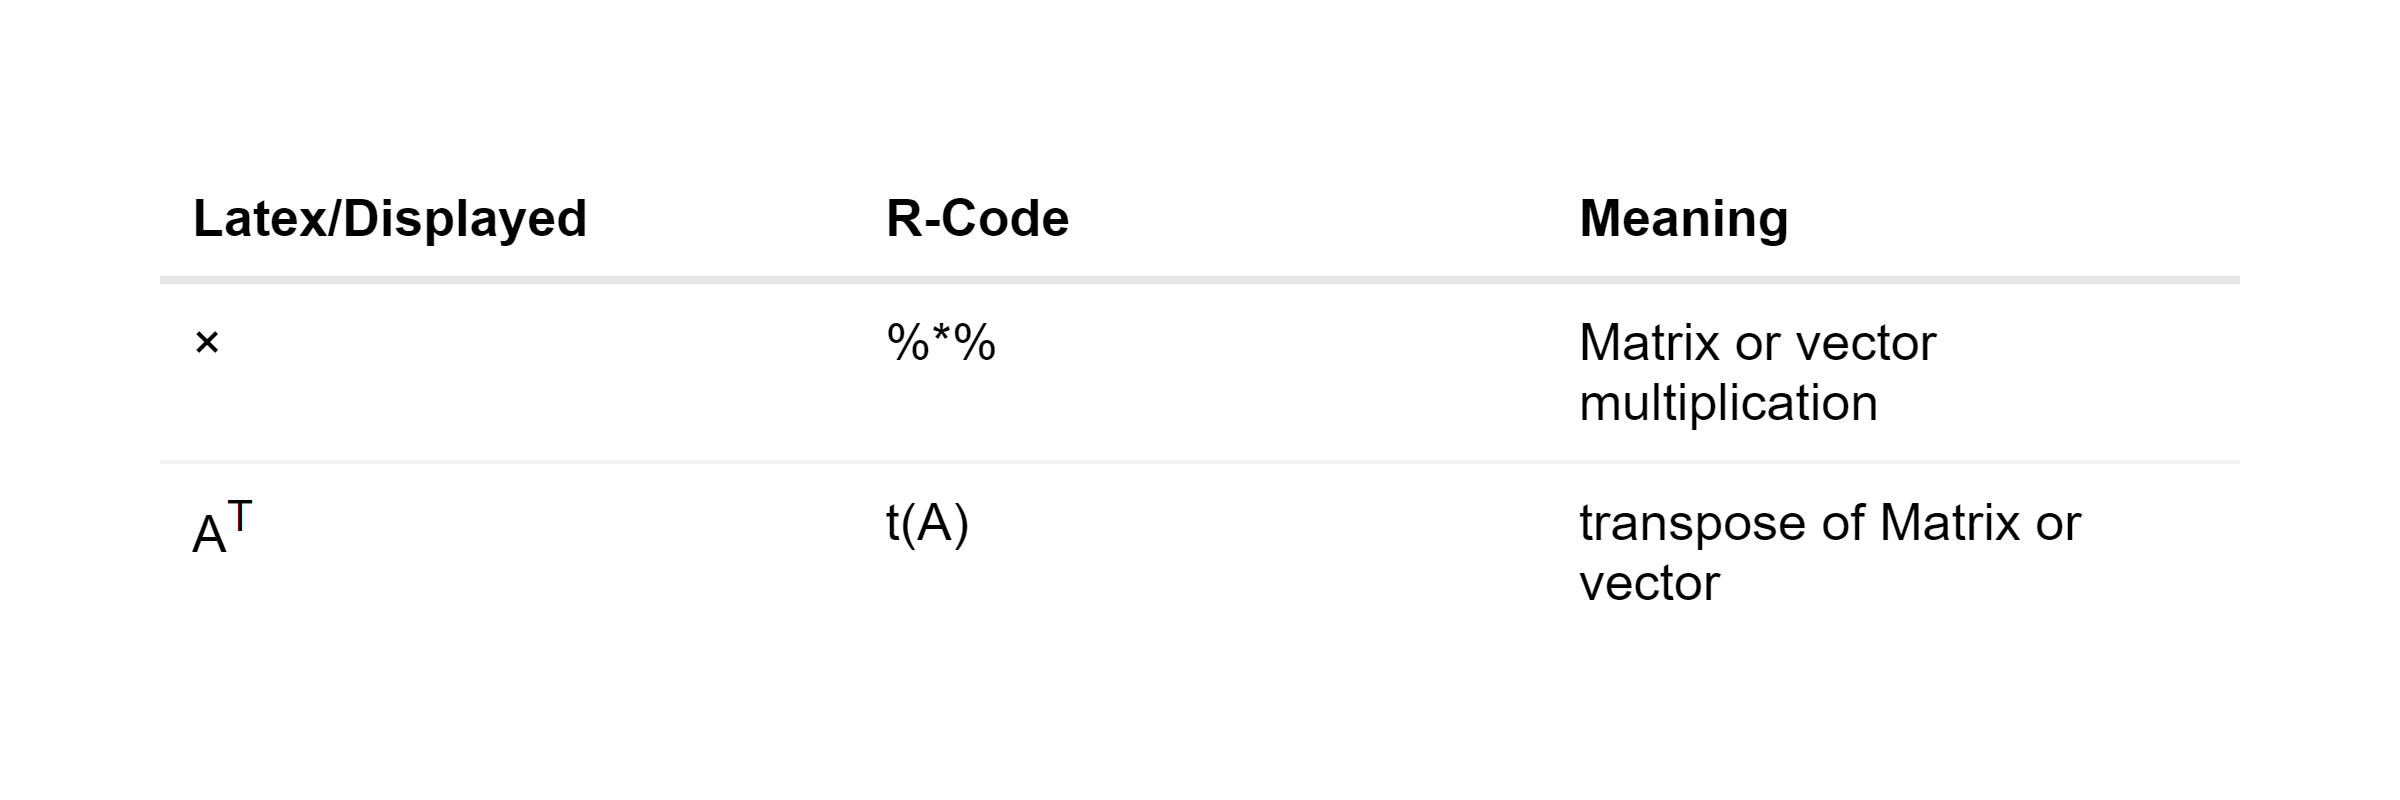
\includegraphics{Master_Thesis_files/figure-latex/unnamed-chunk-2-1}

\hypertarget{abstract}{%
\chapter*{Abstract}\label{abstract}}
\addcontentsline{toc}{chapter}{Abstract}

\pagenumbering{arabic}

Asset allocation aims at constructing portfolios that follow a specific investment strategy, such as index tracking or optimal risk return. These strategies are formulated as optimization problems whose solutions represent an optimal portfolio depending on the strategy. In practice, these problems can be too complicated to be solved directly by deterministic optimization methods, which can lead to simplified models that may contain faulty assumptions or inaccuracies. When this is the case, metaheuristics such as Particle Swarm Optimization (PSO) may be needed. PSO is able to find optimal solutions to complex problems by evaluating random positions in the search space to iteratively approach the optimum. In this thesis, common asset allocation problems are first explained and solved using deterministic optimization methods to generate benchmark problems. After introducing the PSO, it is illustrated with simple examples and the convergence behavior is analyzed before it is subsequently tested on benchmark problems. Then, the PSO and its variants are used to solve optimization problems that cannot be solved by deterministic optimization methods. Finally, the most promising PSO variant is used to solve a discrete index tracking problem considering transaction costs and a rebalancing constraint. Backtests show that this PSO variant can provide time-stable results for such problems.

\hypertarget{introduction}{%
\chapter{Introduction}\label{introduction}}

In the past, active portfolio management was the only approach used, where the portfolio manager actively bought and sold assets to create a portfolio that meets the client's objectives. The goal is to take advantage of assets that are traded at incorrect prices to make a profit. This approach requires a high level of expertise from the portfolio manager, who must be well-informed about the financial market and each asset in the portfolio. However, it is becoming more difficult to spot these false prices as the market becomes more efficient. An efficient market is one where the quoted prices of assets reflect all available information, making it impossible to exploit false prices. This has led to the development of passive portfolio management, a quantitative approach that focuses more on the overall portfolio rather than individual assets. This approach has proven successful, leading to a shift towards passive portfolio management in recent years. In 2014, 18\% of the total net asset value of all funds was passively managed, and this share has increased to 25\% in 2018 \citep{TaDe2019}. The reason for this is complex, but passive management is characterized by many data-driven quantitative strategies, which automate much of the work and save costs by allowing fewer portfolio managers to manage more portfolios. Additionally, passively managed portfolios typically have less rebalancing, which keeps transaction costs lower. In addition to the lower cost, passive portfolios are also often less risky, which is of interest to many investors.

Building a cost-efficient, fully automated portfolio using a quantitative strategy can be challenging due to the complexity of the optimization problems that must be solved. To overcome these challenges, metaheuristics such as Particle Swarm Optimization (PSO) are often used. A metaheuristic is a higher-level optimization method that treats the optimization problem as a black box, only requiring the ability to evaluate the objective function. However, this approach does not provide any guarantee about the quality of the solution, and the runtime is heavily dependent on the time needed to evaluate the function. Thus, it is crucial to thoroughly test a metaheuristic before using it. Research from \citep{BuAd2021} suggests that PSO is more effective than other metaheuristics in various areas, including portfolio optimization problems that cannot be solved by deterministic optimization methods. The goal of this thesis is to apply PSO to financial problems, develop a deep understanding of its behavior, and make the code and data for this thesis freely available for readers to use and apply PSO themselves.

Another objective of this thesis is to provide readers with an introduction to the R programming language, which is particularly well-suited for the purpose of financial data analysis. R is a powerful tool that allows for the implementation of complex algorithms in a user-friendly and intuitive manner. Additionally, R is a widely adopted programming language in various practical domains, including portfolio management, and is frequently used for data analysis and modeling.

The following two chapters present an overview of the software and data utilized, with the aim of ensuring reproducibility. Subsequently, in chapter~\ref{mathfundations}, the mathematical foundations and conventions are outlined. Chapter~\ref{activevspassive} conducts an analysis of active and passive portfolio management, highlighting the advantages of the latter. The subsequent chapter addresses two common objectives of passive portfolio management, namely the index tracking portfolio and the optimal risk return portfolio, which serve as test optimization problems for the application of the PSO algorithm. In order to be able to validate the PSO, a deterministic optimization method is explained in chapter~\ref{analyticalsolver}, which can calculate the optimal solution in the continuous case of the two test problems. The core focus of the thesis, the standard PSO and its behavior, is presented in chapter~\ref{spso}. The test problems from the previous chapter are used to evaluate the performance of the standard PSO. Additionally, a discrete problem that cannot be solved by deterministic optimization methods is demonstrated and solved using the standard PSO. In chapter~\ref{psovariants}, various modifications of the PSO are evaluated by solving a discrete problem, with the standard PSO serving as a benchmark. The results indicate that the local PSO and the self-adjusting velocity PSO are most suitable for such problems. Finally, in chapter~\ref{reallife}, the self-adjusting velocity PSO is applied to solve a real-world index tracking problem, considering transaction costs and rebalancing constraints. The results of the backtests suggest the potential utility of the PSO in solving such complex problems.

\hypertarget{information-about-the-used-software}{%
\chapter{Information about the used Software}\label{information-about-the-used-software}}

All of the thesis was done in the R-Studio IDE using R Markdown extended with the bookdown package. R Markdown allows the user to execute R code in so-called code chunks that are located between the texts. These code chunks can be used, for example, to generate charts that can be displayed in the output instead of the code. Each chunk of code can be cached to avoid time-consuming repetition, and the caching can be disabled to recreate the entire thesis, including all the code and charts it contains. This is helpful primarily for the user to ensure stability of older code, and secondarily for the reader who has access to the R-Markdown files, as they can trace back any analysis or diagram displayed. R-Markdown can produce various formats, such as HTML or PDF output, both of which are used for this thesis. The HTML output is deposited in the corresponding GitHub repository at \citep{GitHub}. The recommended output format of R-Markdown is an HTML file, which has all the capabilities of a web page with HTML, CSS, and Javascript. For this reason, some javascript code has been added to the HTML version to allow the reader to expand important blocks of code alongside the text. The bookdown package is used as a template that contains the necessary styles and formatting to write books with an HTML or PDF output including table of contents, references and more. Together with the possibilities of the programming language R, a reproducible and traceable thesis can be created.

\hypertarget{r-version-and-packages}{%
\section{R Version and Packages}\label{r-version-and-packages}}

The used packages and versions can be found in the table below:

\vspace{0.1cm}\fontsize{11}{13}\selectfont

\begin{verbatim}
R version 4.1.1 (2021-08-10)
Platform: x86_64-w64-mingw32/x64 (64-bit)
Running under: Windows 10 x64 (build 19044)

attached base packages:
[1] stats     graphics  grDevices utils     datasets  methods  
[7] base     

other attached packages:
 [1] ggpubr_0.5.0      metR_0.12.0       gganimate_1.0.7  
 [4] quantmod_0.4.20   TTR_0.24.3        reactable_0.3.0  
 [7] bookdown_0.31     webshot2_0.1.0    corrr_0.4.3      
[10] data.table_1.14.2 pso_1.0.3         plotly_4.10.0    
[13] matrixcalc_1.0-5  Matrix_1.5-3      quadprog_1.5-8   
[16] xts_0.12.1        zoo_1.8-9         rvest_1.0.2      
[19] forcats_0.5.1     stringr_1.4.0     purrr_0.3.4      
[22] tidyr_1.2.0       tibble_3.1.8      ggplot2_3.4.0    
[25] tidyverse_1.3.2   readr_2.1.2       dplyr_1.0.9      
[28] lubridate_1.8.0  

loaded via a namespace (and not attached):
 [1] fs_1.5.2            progress_1.2.2      httr_1.4.3         
 [4] tools_4.1.1         backports_1.2.1     utf8_1.2.2         
 [7] R6_2.5.1            DBI_1.1.3           lazyeval_0.2.2     
[10] colorspace_2.0-2    withr_2.5.0         prettyunits_1.1.1  
[13] tidyselect_1.1.2    processx_3.5.2      curl_4.3.2         
[16] compiler_4.1.1      cli_3.3.0           xml2_1.3.3         
[19] checkmate_2.0.0     scales_1.2.1        digest_0.6.29      
[22] rmarkdown_2.19      pkgconfig_2.0.3     htmltools_0.5.3    
[25] dbplyr_2.2.1        fastmap_1.1.0       htmlwidgets_1.5.3  
[28] rlang_1.0.6         readxl_1.4.0        rstudioapi_0.13    
[31] farver_2.1.0        generics_0.1.3      jsonlite_1.8.0     
[34] car_3.1-1           googlesheets4_1.0.0 magrittr_2.0.3     
[37] Rcpp_1.0.9          munsell_0.5.0       fansi_0.5.0        
[40] abind_1.4-5         lifecycle_1.0.3     stringi_1.7.6      
[43] yaml_2.3.5          carData_3.0-5       grid_4.1.1         
[46] promises_1.2.0.1    crayon_1.5.1        lattice_0.20-44    
[49] haven_2.5.0         chromote_0.1.0      hms_1.1.1          
[52] knitr_1.41          ps_1.6.0            pillar_1.8.0       
[55] ggsignif_0.6.4      reprex_2.0.1        glue_1.6.2         
[58] evaluate_0.19       modelr_0.1.8        tweenr_1.0.2       
[61] vctrs_0.5.1         tzdb_0.3.0          cellranger_1.1.0   
[64] gtable_0.3.0        assertthat_0.2.1    xfun_0.35          
[67] broom_1.0.0         rstatix_0.7.1       later_1.3.0        
[70] googledrive_2.0.0   viridisLite_0.4.0   gargle_1.2.0       
[73] websocket_1.4.0     ellipsis_0.3.2     
\end{verbatim}

\normalsize\vspace{0.1cm}

\hypertarget{reproducibility}{%
\section{Reproducibility}\label{reproducibility}}

Everything in this thesis can be reproduced via the public GitHub repository at \citep{GitHub}. All code sections that use random number generators start with seed 0 to ensure the credibility of the analyses and diagrams shown.

\hypertarget{r-functions}{%
\section{R Functions}\label{r-functions}}

The following functions were created to simplify working with R Markdown and to take advantage of the HTML version of this thesis.

\hypertarget{html_save}{%
\subsection{\texorpdfstring{\texttt{html\_save()}}{html\_save()}}\label{html_save}}

Converts HTML plots to images to display them in the PDF output. This allows the author to use the desired plot packages without having to worry about the different output formats. The disadvantage is, that it is not possible to define the font size within the charts and tables exactly, because the saved images are adjusted to the page width by latex.

\hypertarget{javascript-files}{%
\subsection{javascript files}\label{javascript-files}}

The javascript files are located in the \texttt{www/} folder of the attached GitHub repository and are used for the HTML version of this thesis to make code blocks expandable. This allows the reader to inspect the code used and to follow analyses in detail.

\hypertarget{open-data-sources}{%
\chapter{Open Data Sources}\label{open-data-sources}}

To increase reproducibility, all data are free and can be loaded from the quantmod R package with the function \texttt{getSymbols()}. It is possible to choose between different data sources like yahoo-finance (default), alpha-vantage and others.

\hypertarget{r-functions-1}{%
\section{R Functions}\label{r-functions-1}}

The following functions were created to increase the ease of data collection with the quantmod R package, which can be found in the \texttt{R/} directory in the dedicated GitHub repository \citep{GitHub}.

\hypertarget{get_yf}{%
\subsection{\texorpdfstring{\texttt{get\_yf()}}{get\_yf()}}\label{get_yf}}

This function is the main wrapper for collecting data with \texttt{getSymbols()} from yahoo-finance, and converts prices to returns with the \texttt{pri\_to\_ret()} function explained in section \ref{pritoret}. The output is a list containing prices and returns as \href{https://cran.r-project.org/web/packages/xts/xts.pdf}{xts} objects, which is the usual object in R for storing time series. The arguments that can be passed to \texttt{get\_yf()} are:

\begin{itemize}
\tightlist
\item
  \texttt{tickers}: Vector of symbols (asset names, e.g.~``APPL'', ``GOOG'', \ldots)
\item
  \texttt{from\ ="2018-01-01"}: R Date
\item
  \texttt{to\ =\ "2019-12-31"}: R Date
\item
  \texttt{price\_type\ =\ "close"}: Type of prices to be recorded (e.g.~``open'', ``high'', ``low'', ``close'', ``adjusted'')
\item
  \texttt{return\_type\ =\ "adjusted"}: Type of prices used to calculate the returns (e.g.~``open'', ``high'', ``low'', ``close'', ``adjusted'')
\item
  \texttt{print\ =\ F}: Should the function print the return of \texttt{getSymbols()}
\end{itemize}

\hypertarget{buffer}{%
\subsection{\texorpdfstring{\texttt{buffer()}}{buffer()}}\label{buffer}}

To make data reusable and reduce compilation time, the \texttt{buffer()} function stores the data collected with \texttt{get\_yf()}. It receives an R expression, evaluates it and stores it in the \texttt{buffer\_data/} directory under the specified name. If this name already exists, it loads the R object from the RData files without evaluating the expression. The evaluation and overwriting of the existing RData file can be forced with \texttt{force=T}.

\hypertarget{mathfundations}{%
\chapter{Mathematical Foundations}\label{mathfundations}}

This chapter provides an overview of the mathematical calculations and conventions used in this thesis. It is important to note that most mathematical formulas are written in matrix notation and vectors are interpreted as one-dimensional matrices. In most cases, this will result in a direct translation to R code. All necessary assumptions required for the modeled return structure are listed in this chapter so that any reader can understand the formulas given. It is important to note that reality is too complex and can only be partially modeled. Simple, basic models are used that do not stand up to reality, but these models or variations of them are commonly used in the financial world and have proven to be helpful. The complexity of solving advanced and basic models does not differ for the PSO because the dimension of the objective function is based on the number of elements that can be selected, see chapter \ref{challenges}.

\hypertarget{basic-operators}{%
\section{Basic Operators}\label{basic-operators}}

The programming language R makes it possible to formulate almost all computations in a matrix notation, since the usual matrix operators and element-wise operators are already efficiently implemented in base R. Element-wise operators are not considered standard in mathematics, so they are defined in more detail in this section. The representation of calculations in a matrix notation helps the user to keep the overview, because the formulas are more compact and in addition, these operators are already implemented efficiently in base R, which makes them more performant than simple for-loops. The operators used here can be found in the table below and are intended to establish the relationship between the notation in the text, in the R code and their meaning:

\begin{figure}[H]
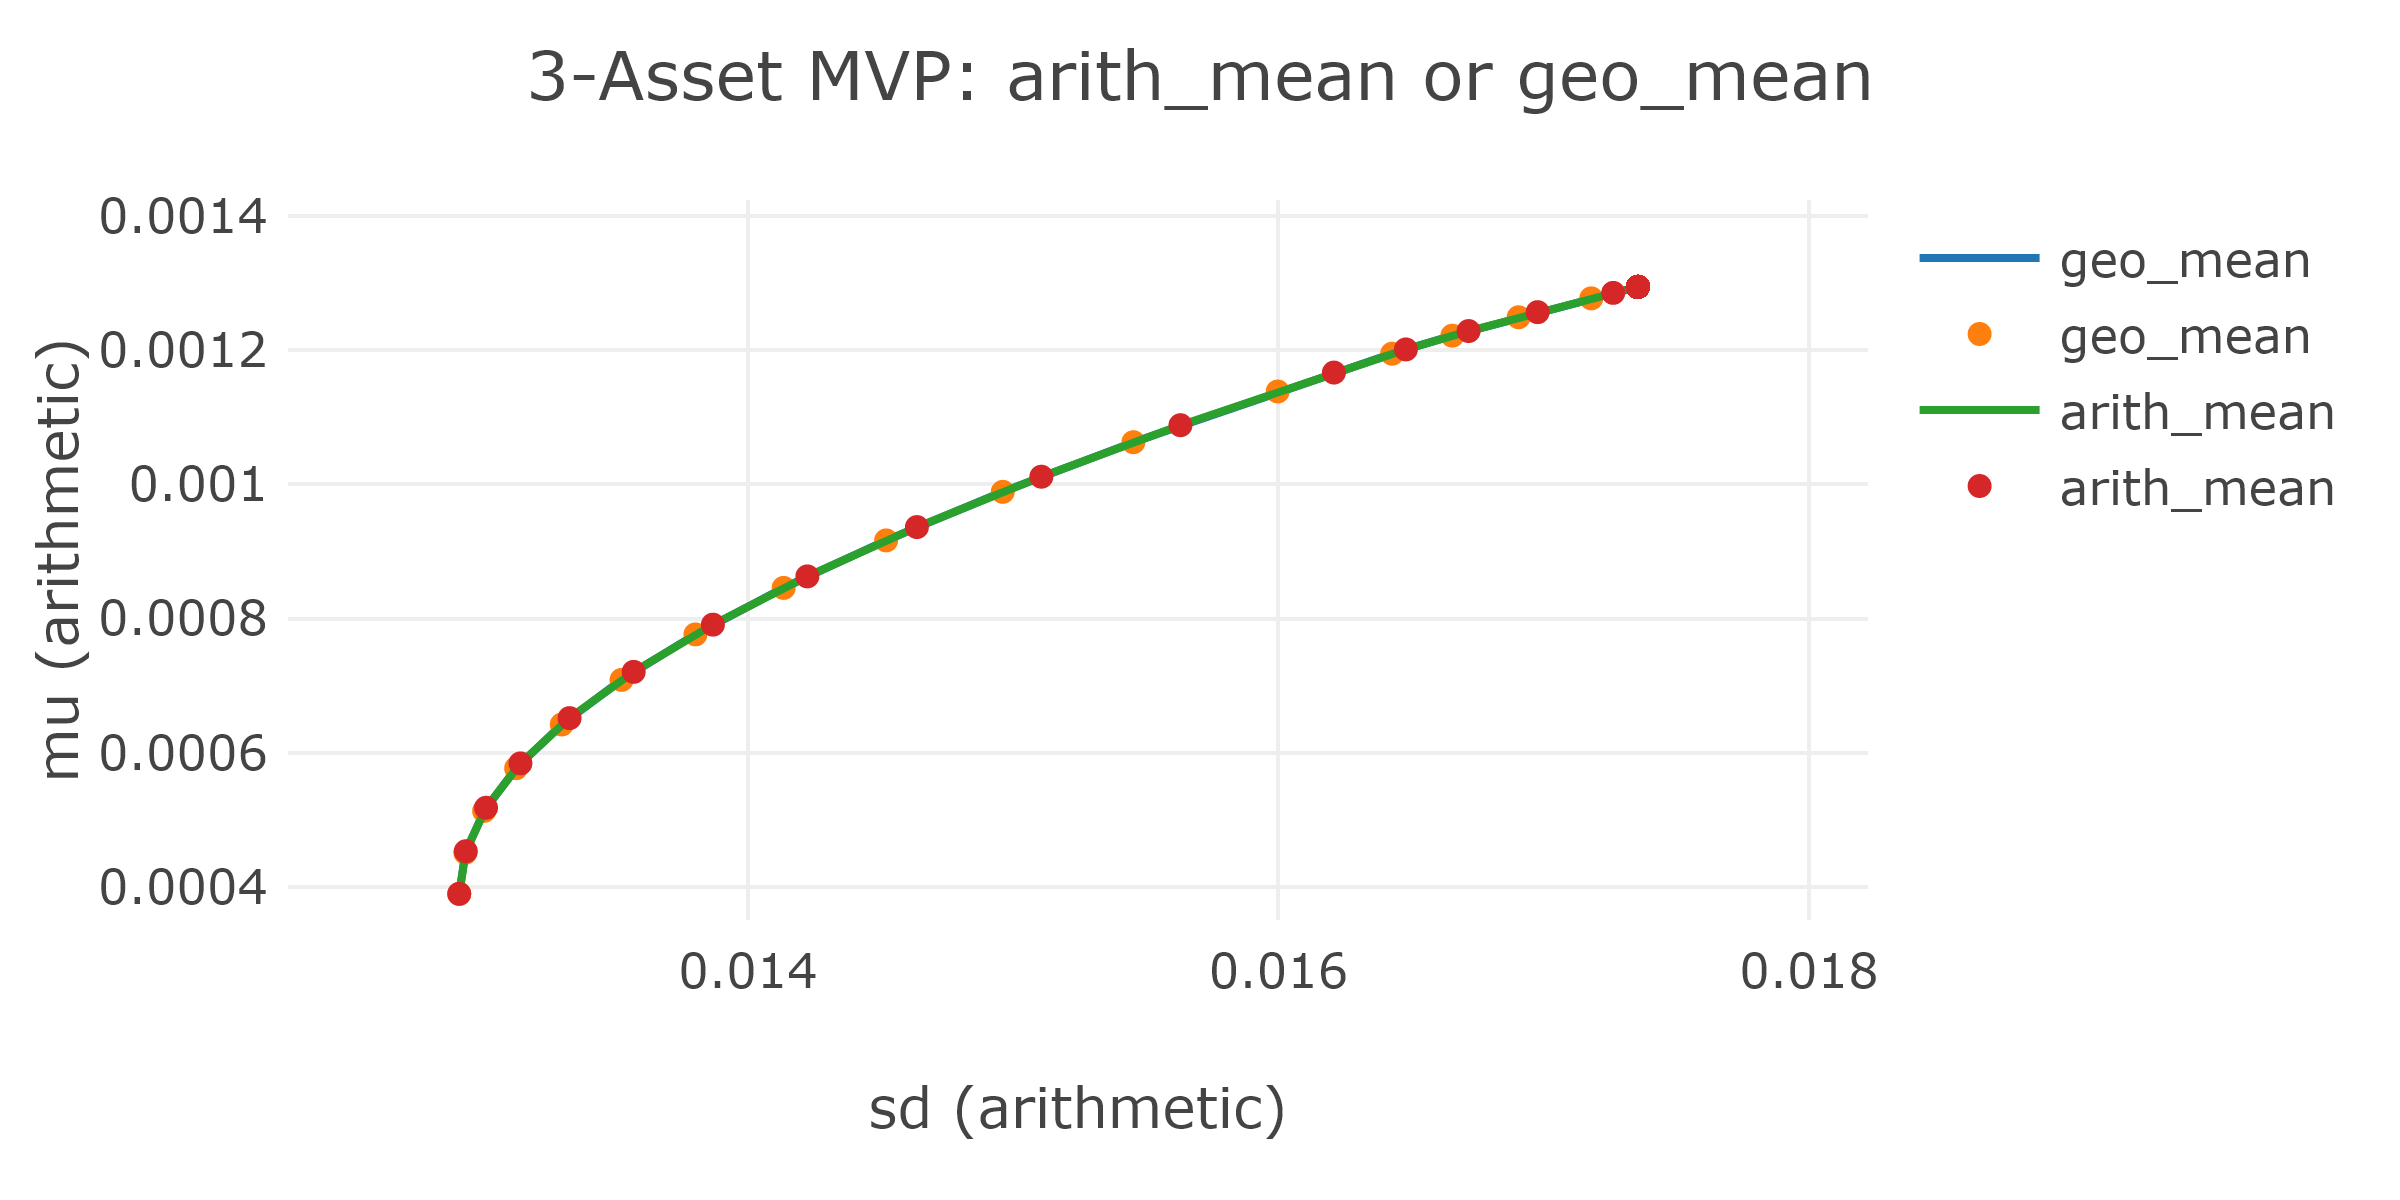
\includegraphics{Master_Thesis_files/figure-latex/unnamed-chunk-4-1} \caption{List of used operators and their meanings}\label{fig:unnamed-chunk-4}
\end{figure}

For a better understanding of the operators listed, the following examples are intended to illustrate the resulting dimensions and provide insight into the use of these operators.

The matrix product is defined by the following mapping:

\[\times: \ \ \mathbb{R}^{x \times y} \times \mathbb{R}^{y \times z} \rightarrow \mathbb{R}^{x \times z},\]

with an example:

\[ 
\begin{bmatrix}a_{1,1} &\cdots  & a_{1,y} \\ \vdots & \ddots & \vdots  \\ a_{x,1} & \cdots & a_{x,y} \end{bmatrix}
\times
\begin{bmatrix}b_{1,1} &\cdots  & b_{1,z} \\ \vdots & \ddots & \vdots  \\ b_{y,1} & \cdots & b_{y,z} \end{bmatrix}
=
\begin{bmatrix} \sum_{i=1}^y a_{1, i} \cdot  b_{i,1} &\cdots  & \sum_{i=1}^y a_{1, i} \cdot  b_{i,z} \\ \vdots & \ddots & \vdots  \\ \sum_{i=1}^y a_{x, i} \cdot  b_{i,1}  & \cdots & \sum_{i=1}^y a_{x, i} \cdot  b_{i,z} \end{bmatrix}.
\]

In the case of vectors, the matrix product has the following mapping:

\[\times: \ \ \mathbb{R}^{1 \times N} \times \mathbb{R}^{N \times 1} \rightarrow \mathbb{R},\]

with an example:

\[
\begin{bmatrix}a_{1} &\cdots  &  a_{N}\end{bmatrix}
\times
\begin{bmatrix}b_{1}\\ \vdots \\  b_{N}\end{bmatrix}
=
\sum_{i=1}^N a_i \cdot  b_i.
\]

The outer product is defined by the following mapping:

\[\otimes: \ \ \mathbb{R}^{x \times 1} \times \mathbb{R}^{1 \times y} \rightarrow \mathbb{R}^{x \times y},\]

with an example:

\[
\begin{bmatrix}a_{1}\\ \vdots \\ a_{x}\end{bmatrix}
\otimes
\begin{bmatrix}b_{1} &\cdots  & b_{y}\end{bmatrix}
=
\begin{bmatrix}a_{1} \cdot b_{1} &\cdots  & a_{1} \cdot b_{y} \\ \vdots & \ddots & \vdots  \\ a_{x} \cdot b_{1}  & \cdots & a_{x} \cdot b_{y} \end{bmatrix}.
\]

This thesis is specified for the use of R, so element-wise operators are very important to make code comparable with formulas. In mathematics, these operators are not common. For this reason, they must be explicitly specified. All element-wise operators work in the same way. Assuming that \(\square\) is one of the four element-wise operators, then the mapping is defined as follows:

\begin{align*}
\square &: \ \ R^{x \times y} \times R^{x \times y}  \rightarrow R^{x \times y}\\
\text{or }\ \square &: \ \ R^{x} \times R^{x \times y}  \rightarrow R^{x \times y}\\
\text{or }\ \square &: \ \ R \times R^{x \times y}  \rightarrow R^{x \times y},
\end{align*}

with examples respectively:

\[
\begin{bmatrix}a_{11} &\cdots  & a_{1y} \\ \vdots & \ddots & \vdots  \\ a_{x1} & \cdots & a_{xy} \end{bmatrix}
\square
\begin{bmatrix}b_{11} &\cdots  & b_{1y} \\ \vdots & \ddots & \vdots  \\ b_{x1} & \cdots & b_{xy} \end{bmatrix}
=
\begin{bmatrix}a_{11} \square b_{11} &\cdots  & a_{1y} \square b_{1y} \\ \vdots & \ddots & \vdots  \\ a_{x1} \square b_{x1}  & \cdots & a_{xy} \square b_{xy} \end{bmatrix}
\]

or
\vspace{0.2cm}
\[
\begin{bmatrix}a_{1} \\ \vdots \\ a_{x} \end{bmatrix}
\square
\begin{bmatrix}b_{11} &\cdots  & b_{1y} \\ \vdots & \ddots & \vdots  \\ b_{x1} & \cdots & b_{xy} \end{bmatrix}
=
\begin{bmatrix}a_{1} \square b_{11} &\cdots  & a_{1} \square b_{1y} \\ \vdots & \ddots & \vdots  \\ a_{x} \square b_{x1}  & \cdots & a_{x} \square b_{xy} \end{bmatrix}
\]

or
\vspace{0.2cm}
\[
a \ 
\square
\begin{bmatrix}b_{11} &\cdots  & b_{1y} \\ \vdots & \ddots & \vdots  \\ b_{x1} & \cdots & b_{xy} \end{bmatrix}
=
\begin{bmatrix}a \square b_{11} &\cdots  & a \square b_{1y} \\ \vdots & \ddots & \vdots  \\ a \square b_{x1}  & \cdots & a \square b_{xy} \end{bmatrix}.
\]

The operators on the right side of the above example equations corresponds to the common operators in scalar.

\hypertarget{formula-conventions}{%
\section{Formula Conventions}\label{formula-conventions}}

In mathematics, random variables are written in capital letters, which also applies to matrices. In order to allow an unambiguous assignment, the random variables are written in bold and in capital letters. For example, \(A\) should represent a matrix and \(\pmb{A}\) should represent a random variable.

\hypertarget{return-calculation}{%
\section{Return Calculation}\label{return-calculation}}

Any portfolio optimization strategy based on historical data must start with returns. These returns are calculated using \href{https://www.investopedia.com/terms/a/adjusted\%20closingprice.asp}{adjusted closing prices}, which show the percentage change over time. Adjusted closing prices reflect dividends and are adjusted for stock splits and rights offerings. These returns are essential for comparing assets and analyzing dependencies.

\hypertarget{simple-returns}{%
\subsection{Simple Returns}\label{simple-returns}}

The default time frame for all raw data in this thesis is a working day, prices are always measured in the evening, and only simple returns are used. Assuming that there is an asset with price \(p_{t_i}\) on working day \(t_i\) and price \(p_{t_{i+1}}\) on the following working day \(t_{i+1}\), the simple rate of return for \(t_{i+1}\) can be calculated as follows:

\[
  r_{t_{i+1}} = \frac{p_{t_{i+1}}}{p_{t_i}}-1.
\]

\hypertarget{markowitz-modern-portfolio-theory}{%
\section{Markowitz Modern Portfolio Theory}\label{markowitz-modern-portfolio-theory}}

In 1952, Harry Markowitz published his first seminal paper, which had a significant impact on modern finance, primarily by outlining the implications of diversification and efficient portfolios in \citep{Mark1952}. He later published a monograph on a more in-depth analysis of his findings in \citep{Mark1959}. The definition of an efficient portfolio is a portfolio that has either the maximum expected return for a given risk target or the minimum risk for a given expected return target. A simple quote to define diversification might be, ``A portfolio has the same return but less variance than the sum of its parts.'' This is the case when assets are not perfectly correlated, as poor and good performances can offset each other, reducing the likelihood of extreme events. For more information, see \citep{Mari2005}.

\hypertarget{assumptions-of-markowitz-portfolio-theory}{%
\subsection{Assumptions of Markowitz Portfolio Theory}\label{assumptions-of-markowitz-portfolio-theory}}

This thesis focuses on problems derived from Markowitz's portfolio theory, without closed form solutions, which are studied in \citep{Mari2005} by excluding short selling. The following list contains these types of Markowitz assumptions according to \citep{Mari2005} and \citep{Mark1952}:

\begin{itemize}
\tightlist
\item
  Perfect market without taxes or transaction costs
\item
  Assets are infinitely divisible
\item
  Short sales are disallowed
\item
  Expected returns, variances and covariances contain all information
\item
  Investors are risk-averse, they will only accept greater risk if they
  are compensated with a higher expected return
\end{itemize}

The assumption that the returns are normally distributed is not required, but is assumed in this case to simplify the problem. It is obvious that these assumptions are unrealistic in reality. More details on the requirements for using other distributions can be found in \citep{Mari2005}.

\hypertarget{portfolio-math}{%
\section{Portfolio Math}\label{portfolio-math}}

Proofs of the basic calculations required for portfolio optimization, as shown in \citep{Eric2021}, are provided in this section. Returns are presented differently than in most sources, as this is the most common data format used in practice. Suppose there are \(N\) assets described by a return vector \(\pmb{R}\) of random variables, and the relative contribution to the net asset value of the portfolio is described by the weight vector \(w\), which typically satisfies \(\sum w = 1\):

\[
  \pmb{R} = 
  \begin{bmatrix}
    \pmb{R}_{1} & \pmb{R}_{2} & \cdots & \pmb{R}_{N}  
 \end{bmatrix}
 , \ \ 
 w = 
  \begin{bmatrix}
    w_{1} \\ 
    w_{2} \\
    \vdots \\
    w_{N}  
 \end{bmatrix}.
\]

In this thesis, each return is simplified as being normally distributed with \(\pmb{R}_i = \mathbb{N}(\mu_i, \sigma_i^2)\). As a result, linear combinations of normally distributed random variables are jointly normally distributed and have a mean, variance, and covariance that can be used to fully describe them.

\hypertarget{expected-returns}{%
\subsection{Expected Returns}\label{expected-returns}}

The following formula can be used to get the expected returns of a vector with normally distributed random variables \(\pmb{R} \in \mathbb{R}^{1\times N}\):

\begin{align*}
  E[\pmb{R}] &=
  \begin{bmatrix}
    E[\pmb{R}_{1}] & E[\pmb{R}_{2}] & \cdots & E[\pmb{R}_{N}]  
 \end{bmatrix}\\
 &=
 \begin{bmatrix}
    \mu_{1} & \mu_{2} & \cdots & \mu_{N} 
 \end{bmatrix}
 =
 \mu
\end{align*}

and \(\mu_i\) can be estimated in R using historical data and the formula for the geometric mean of returns (also called compound returns). The function to calculate the geometric mean of returns from an xts object can be found in section \ref{geomeanret}.

\hypertarget{expected-portfolio-returns}{%
\subsection{Expected Portfolio Returns}\label{expected-portfolio-returns}}

The following equation can be used to obtain the expected portfolio return \(E[\pmb{R}_p]\) using the formulations from the section above and a weighting vector \(w\) (e.g.~portfolio weights):

\begin{align*}
E[\pmb{R}_p] &=
 E[\pmb{R} \times w] = 
 E[\pmb{R}] \times w \\
 &= 
  \begin{bmatrix}
    E[\pmb{R}_{1}] & E[\pmb{R}_{2}] & \cdots & E[\pmb{R}_{N}]
 \end{bmatrix}
  \times 
  \begin{bmatrix}
    w_{1} \\ 
    w_{2} \\
    \vdots \\
    w_{N}  
 \end{bmatrix} \\
 &=
   \begin{bmatrix}
    \mu_{1} & \mu_{2} & \cdots & \mu_{N}
 \end{bmatrix}
  \times 
  \begin{bmatrix}
    w_{1} \\ 
    w_{2} \\
    \vdots \\
    w_{N}  
 \end{bmatrix} \\
 &=
 \mu_{1} \cdot w_1 + \mu_{2} \cdot w_2 + \cdots + \mu_{N} \cdot w_{N} 
 =
 \mu_P
\end{align*}

\hypertarget{covariance}{%
\subsection{Covariance}\label{covariance}}

The general formula of the covariance matrix \(\textstyle\sum\) of a random vector \(\pmb{R}\) with \(N\) normally distributed elements and \(\sigma_{i,j}\) as correlation of two distinct values is described as follows:

\begin{align*}
  Cov(\pmb{R}) &= E[(\pmb{R}-\mu)^T \otimes (\pmb{R}-\mu)] \\
  &=   \begin{bmatrix}
    \sigma_1^2 & \sigma_{1,2} & \cdots & \sigma_{1,N} \\
    \sigma_{2, 1} & \sigma_2^2 & \cdots & \sigma_{2, N} \\
    \vdots  & \vdots & \ddots & \vdots \\
    \sigma_{N, 1} & \sigma_{N, 2} & \cdots & \sigma_N^2 \\
 \end{bmatrix}\\
  &=\textstyle\sum
\end{align*}

and can be estimated in R using the base function \texttt{cov()} and historical data. The function \texttt{cov\_()} explained in section \ref{covfun} can be used to calculate the covariance using the geometric mean to estimate the expected returns.

\hypertarget{portvar}{%
\subsection{Portfolio Variance}\label{portvar}}

Let \(\pmb{R}\) be a random vector with \(N\) normally distributed elements and \(w\) a weight vector. Assuming that the covariance matrix \(\sum\) of \(\pmb{R}\) is known, the variance of the linear combination of \(\pmb{R}\) can be calculated as follows:

\begin{align*}
  Var(\pmb{R} \times w) &= E[(\pmb{R} \times w - \mu \times w)^2] \\
  &= E[((\pmb{R} - \mu) \times w)^2]
\end{align*}

Since \((\pmb{R} - \mu) \times w\) is a scalar, it can be transformed from \(((\pmb{R} - \mu) \times w)^2\) to \mbox{$((\pmb{R} - \mu) \times w)^T \cdot ((\pmb{R} - \mu) \times w)$} and results in:

\begin{align*}
  Var(\pmb{R} \times w) &= E[((\pmb{R} - \mu) \times w)^T \cdot ((\pmb{R} - \mu) \times w)]\\ 
  &= E[(w^T \times (\pmb{R} - \mu)^T) \cdot ((\pmb{R} - \mu) \times w)]\\ 
  &= w^T \times E[(\pmb{R} - \mu)^T \otimes (\pmb{R} - \mu)] \times w \\
  &= w^T \times Cov(\pmb{R}) \times w \\
  &= w^T \times \textstyle\sum \times w.
\end{align*}

The same is true for an estimate of \(Var(\pmb{R} \times w)\) by using the estimate of \(\textstyle\sum\).

\hypertarget{portfolioreturns}{%
\subsection{Portfolio Returns}\label{portfolioreturns}}

Suppose there are \(N\) assets that form a portfolio with weights \(w_{t_0}\) at time step \(t_0\), and the portfolio is to go through several time steps until \(t_T\) without rebalancing. What are the portfolio returns at each time step \(t_i\)? Clearly, assets with higher performance at the current time step will have a higher weight at the next time step. This can be done by adjusting the weights after each time step as a function of returns. Suppose we have a complete portfolio \(\textstyle\sum w_{t_0} = 1\) with a return matrix \(R \in \mathbb{R}^{T \times N}\) and we want to calculate the portfolio returns \(R_{t_1}^P\). This can be done with the following two steps:

\begin{align*}
  Z_{t_1} &= (1+R_{t_1}) \cdot w_{t_0}^T\\
  R_{t_1}^P &= \sum_{n = 1}^N Z_{t_1, n} - 1.
\end{align*}

And since the portfolio was full in \(t_0\), the adjusted weights in \(t_1\) are \(w_{t_1} = Z_{t_1}/\sum_{n = 1}^N Z_{t_1, n}\) (element-wise division). These new weights can be used in the next time step to replace the weights \(w_{t_0}\) in the above formula. The recursive formula for holding a portfolio with weights \(\textstyle\sum w_{t_0} = 1\) in \(t_0\) and return matrix \(R \in \mathbb{R}^{T \times N}\), has portfolio return \(R_{t_i}^P = \textstyle\sum_{n = 1}^N Z_{t_i, n} - 1\) in \(t_i\) with \(i=1, 2, \cdots, T\) for:

\[
  Z_{t_i} =
  \begin{cases}
  (1+R_{t_i})\cdot w_{t_0}^T &\text{ if }i=1\\
  (1+R_{t_i})\cdot \frac{Z_{t_{i-1}}}{\sum_{n = 1}^N Z_{t_{i-1, n}}} &\text{ if }i>1.
  \end{cases}
\]

The requirement that the portfolio is full can be achieved by adding an additional weight to \(w_{t_0}\), which includes the residual \(1-\textstyle\sum w_{t_0}\) and an additional zero return vector to \(R\). This calculation of portfolio returns is implemented in the function \texttt{calc\_portfolio\_returns()} below.

\hypertarget{r-functions-2}{%
\section{R Functions}\label{r-functions-2}}

The following functions serve the purpose to encapsulate mathematical calculations and to make the calculations reusable. All functions are located in the dedicated GitHub repository inside the \texttt{R/} folder.

\hypertarget{covfun}{%
\subsection{\texorpdfstring{\texttt{cov\_()}}{cov\_()}}\label{covfun}}

This function extends the base R function \texttt{cov()} by allowing the user to pass an expected value vector. This is used to calculate the covariance with expected returns based on the geometric mean instead of the arithmetic mean.

\hypertarget{pritoret}{%
\subsection{\texorpdfstring{\texttt{pri\_to\_ret()}}{pri\_to\_ret()}}\label{pritoret}}

This function calculates the simple returns of a given xts object containing prices. Before that, missing prices are replaced by the previous value in the respective column.

\hypertarget{ret_to_cumret}{%
\subsection{\texorpdfstring{\texttt{ret\_to\_cumret()}}{ret\_to\_cumret()}}\label{ret_to_cumret}}

This function is used to calculate cumulative returns normalized to 100 from a given xts object containing returns. This function is often used before plotting return time series.

\hypertarget{geomeanret}{%
\subsection{\texorpdfstring{\texttt{ret\_to\_geomeanret()}}{ret\_to\_geomeanret()}}\label{geomeanret}}

The geometric mean of returns is a better estimator than the arithmetic mean of returns because it captures the exact mean price changes over a period of time. The variance estimated from the daily returns is a daily variance, so the returns must have the same time base. This can be done by calculating the geometric mean of the returns from multiple daily returns. Assuming there is an asset with returns \(r_1 = 0.01\), \(r_2=-0.03\), and \(r_3=0.02\), it follows that the geometric mean return \(r^{geom}\) can be calculated as:

\[
  r^{geom} = ((1+r_1) \cdot (1+r_2) \cdot (1+r_3))^{1/3}-1 = -0.0002353887
\]

And the advantage is that it is a daily average return that gives exactly the same result as the real returns, that is:

\[
  (1+r^{geom})^3 = (1+r_1) \cdot (1+r_2) \cdot (1+r_3)
\]

This is not the case with the arithmetic mean of the returns. The general formula for calculating the geometric mean return of \(n\) days is:

\[
  r^{geom} = (\prod_{i=1}^n (1+r_i))^{\frac{1}{n}}-1
\]

and as R code:

\vspace{0.1cm}\fontsize{11}{12}\selectfont

\begin{Shaded}
\begin{Highlighting}[]
\NormalTok{ret\_to\_geomeanret }\OtherTok{\textless{}{-}} \ControlFlowTok{function}\NormalTok{(xts\_ret)\{}
  \FunctionTok{sapply}\NormalTok{((}\DecValTok{1}\SpecialCharTok{+}\NormalTok{xts\_ret), prod)}\SpecialCharTok{\^{}}\NormalTok{(}\DecValTok{1}\SpecialCharTok{/}\FunctionTok{nrow}\NormalTok{(xts\_ret))}\SpecialCharTok{{-}}\DecValTok{1}
\NormalTok{\}}
\end{Highlighting}
\end{Shaded}

\normalsize\vspace{0.1cm}

\hypertarget{calc_portfolio_returns}{%
\subsection{\texorpdfstring{\texttt{calc\_portfolio\_returns()}}{calc\_portfolio\_returns()}}\label{calc_portfolio_returns}}

This is the implementation of a vectorial calculation of portfolio returns over multiple periods with a weighting vector \texttt{weights} at \(t_0\) and no re-balancing:

\vspace{0.1cm}\fontsize{11}{12}\selectfont

\begin{Shaded}
\begin{Highlighting}[]
\NormalTok{calc\_portfolio\_returns }\OtherTok{\textless{}{-}} 
  \ControlFlowTok{function}\NormalTok{(xts\_returns, weights, }\AttributeTok{name=}\StringTok{"portfolio"}\NormalTok{)\{}
  \ControlFlowTok{if}\NormalTok{(}\FunctionTok{sum}\NormalTok{(weights)}\SpecialCharTok{!=}\DecValTok{1}\NormalTok{)\{}
\NormalTok{    xts\_returns}\SpecialCharTok{$}\NormalTok{temp\_\_\_X1 }\OtherTok{\textless{}{-}} \DecValTok{0}
\NormalTok{    weights }\OtherTok{\textless{}{-}} \FunctionTok{c}\NormalTok{(weights, }\DecValTok{1}\SpecialCharTok{{-}}\FunctionTok{sum}\NormalTok{(weights))}
\NormalTok{  \}}
\NormalTok{  res }\OtherTok{\textless{}{-}} \FunctionTok{cumprod}\NormalTok{((}\DecValTok{1}\SpecialCharTok{+}\NormalTok{xts\_returns)) }\SpecialCharTok{*} \FunctionTok{matrix}\NormalTok{(}
    \FunctionTok{rep}\NormalTok{(weights, }\FunctionTok{nrow}\NormalTok{(xts\_returns)), }\AttributeTok{ncol=}\FunctionTok{length}\NormalTok{(weights), }\AttributeTok{byrow=}\NormalTok{T)}
\NormalTok{  res }\OtherTok{\textless{}{-}} \FunctionTok{xts}\NormalTok{(}
    \FunctionTok{rowSums}\NormalTok{(res}\SpecialCharTok{/}\FunctionTok{c}\NormalTok{(}\DecValTok{1}\NormalTok{, }\FunctionTok{rowSums}\NormalTok{(res[}\SpecialCharTok{{-}}\FunctionTok{nrow}\NormalTok{(xts\_returns),])))}\SpecialCharTok{{-}}\DecValTok{1}\NormalTok{, }
    \AttributeTok{order.by=}\FunctionTok{index}\NormalTok{(xts\_returns)) }\SpecialCharTok{\%\textgreater{}\%} 
    \FunctionTok{setNames}\NormalTok{(., name)}
  \FunctionTok{return}\NormalTok{(res)}
\NormalTok{\}}
\end{Highlighting}
\end{Shaded}

\normalsize\vspace{0.1cm}

This function has the same results as the \texttt{Return.portfolio()} function from the \texttt{PortfolioAnalytics} package.

\hypertarget{activevspassive}{%
\chapter{Active vs.~Passive Portfolio Management}\label{activevspassive}}

An active portfolio manager seeks to achieve positive alpha, i.e., excess returns relative to the market, by applying his knowledge, experience, and in-depth analysis of individual assets. Therefore, the manager assumes that the market is not efficient and tries to select mispriced assets to generate excess returns. The passive portfolio manager, on the other hand, assumes that the market is efficient, that is, that prices reflect all available information, and attempts to replicate the average market return by building a diversified portfolio. He knows that stock movements follow a ``random walk'' and are therefore unpredictable for any individual stock. The passive portfolio manager achieves his goal with a quantitative strategy and assumes that the results will be stable over time. ETFs that aim to track indices are classified as passively managed in this thesis.

The question is which of the two types of portfolio management is preferable.

\hypertarget{results-of-the-literature}{%
\section{Results of the Literature}\label{results-of-the-literature}}

Researchers Fama and French studied the returns of active and passive portfolio management by designing factor models that led to a wide range of models commonly used today to analyze the causes of returns. Their theory states that passive investors earn passive returns that have an alpha of zero before costs. This implies that active investors also collectively have an alpha of zero before costs. This means that if some active investors have a positive alpha, other active investors have achieved a negative alpha. Indeed, Fama and French analyzed this behavior in more detail in \citep{FaFr2010}, finding that value-weighted professionally managed mutual funds that invest primarily in the U.S. equity market have a slightly positive alpha before costs at the expense of active investors outside of professionally managed mutual funds. In addition, Fama and French attempted to use regression models to distinguish between luck and skill in active portfolio management. Their results suggest that some active managers in the top percentiles have sufficient skill to cover costs over the long run. Nevertheless, actively managed funds in the top percentiles have an estimated alpha after costs that is close to zero, which is also true for large, efficiently managed passive funds.

Similar results were obtained in \citep{PaHi2016}, which analyzed European and U.S. active and passive funds. The results show that none of them is superior by cost. They suggest comparing active and passive managed funds on a case-by-case basis by considering all expenses. When the tax advantages of passively managed funds are taken into account, they can be slightly advantageous for investors with a long investment horizon.

A different viewpoint was taken in \citep{RaSh2004}, analyzing the value of active portfolio management. The results show that some actively managed funds generate large positive excess returns. These funds often had a small number of assets, which could be due to the fact that portfolio managers had more capacity to analyze each asset in detail. This suggests that experienced portfolio managers can indeed generate stable excess returns over time. But in contrast, these same funds charge increased fees that negate the benefits to clients.

The last source analyzed passive and active EU equity funds in \citep{TaDe2019}. It was observed that the top 25\% of actively managed funds outperform passively managed funds, but the group of actively managed funds changes over time. This leads to increased risks for investors as they need to buy and sell funds at the right time. They also analyzed the increasing popularity of passively managed funds, whose market capitalization increased by more than 61\% between 2014 and 2018. On the other hand, the market capitalization of actively managed funds increased by only 16\% overall, indicating a significant shift toward passively managed funds. After comparing the aggregated performance after costs between 2009 and 2018, it was found that the group of actively managed funds with smaller market capitalization lagged behind the larger ones and the larger ones lagged behind the passively managed funds.

\hypertarget{aggregation-of-the-literature}{%
\section{Aggregation of the Literature}\label{aggregation-of-the-literature}}

In summary, it can be said that both strategies have their justification. On the one hand, it was shown that there are actively managed funds that can constantly generate positive alpha and share this in part with the investor. But this refers only to a small part of the actively managed funds. Passively managed funds cannot be expected to generate excess returns, but on average they often meet their benchmark tracking target. Since actively managed funds often incur higher costs, they must constantly beat the market, which carries an implicit risk. In particular, it was shown that many of the active funds with positive performance only managed to do so within a certain period of time before underperforming again. From these results, one could conclude that passively managed funds carry less risk for investors in the long run. Especially if external factors such as tax relief also apply. As passive management has steadily gaine popularity in recent years, it is also more future-oriented to develop and improve these strategies.

\hypertarget{challenges}{%
\chapter{Challenges of Passive Portfolio Management}\label{challenges}}

In this chapter, two common challenges of passive portfolio management are analyzed to create simple use cases for testing the PSO. The first challenge is the mean-variance portfolio (MVP) from Markowitz's modern portfolio theory, which, simply put, is an optimal allocation of assets in terms of risk and return. The second challenge is the index tracking problem, which attempts to construct a portfolio with minimal tracking error to a given benchmark.

\hypertarget{mean-variance-portfolio-mvp}{%
\section{Mean-Variance Portfolio (MVP)}\label{mean-variance-portfolio-mvp}}

Markowitz showed that diversifying risk across multiple assets reduces overall portfolio risk. This result was the beginning of the widely used modern portfolio theory, which uses mathematical models to create portfolios with minimal variance for a given return target. All such optimal portfolios for a given return target are called efficient and constitute the efficient frontier. The problem behind Markowitz's original MVP without constraints can be solved in a closed form, which is explained in \citep{Eric2021}. This type of MVP has no practical use, so only MVP problems with constraints and without closed forms are of interest in this thesis.

\hypertarget{mvp-problem}{%
\subsection{MVP: Problem}\label{mvp-problem}}

Let there be \(N\) assets and their returns on \(T\) different days, creating a return matrix \(R \in \mathbb{R}^{T \times N}\). Each element \(R_{t,i}\) contains the return of the \(i\)-th asset on day \(t\). The estimated covariance matrix of the returns is \(\textstyle\sum \in \mathbb{R}^{N \times N}\) and the estimation of the expected returns are \(\mu \in \mathbb{R}^{N}\). The MVP problem with the risk aversion parameter \(\lambda \in [0,1]\), as shown in \citep{Mari2005}, can be formalized as follows:

\begin{equation} 
\underset{w}{min} \ \ \ \lambda \ w^T \textstyle\sum w - (1-\lambda) \ \mu^T w.
\label{eq:MVP}
\end{equation}

The risk aversion parameter \(\lambda\) defines the tradeoff between risk and return. With \(\lambda = 1\), the minimization problem contains only the variance term, leading to a minimum variance portfolio, and \(\lambda = 0\) transforms the problem into a minimization of negative expected returns, leading to a maximum return portfolio. All possible portfolios created by \(\lambda \in [0, 1]\) define the efficient frontier.

\hypertarget{example-mvp}{%
\subsection{Example MVP}\label{example-mvp}}

All possible MVP's together define the efficient frontier, which is analyzed in this section without going into the details of its calculation. This example uses three assets (stocks: IBM, Google, Apple) and calculates the MVP for each \(\lambda\). First, the daily returns of these three assets from 2018-01-01 to 2019-12-31 are loaded.

The cumulative daily returns are:

\begin{figure}[H]
\includegraphics{Master_Thesis_files/figure-latex/MVPex2-1} \caption{Cumulative daily returns of IBM, Apple and Google}\label{fig:MVPex2}
\end{figure}

The expected daily returns and the covariance matrix for the three assets can be estimated using the formulas from chapter \ref{mathfundations}:

\vspace{0.1cm}\fontsize{11}{12}\selectfont

\begin{verbatim}
estimation of expected daily returns:
         AAPL           IBM          GOOG 
 0.0011434117 -0.0001059161  0.0004870292 

estimation of positiv definite covariance matrix:
             AAPL          IBM         GOOG
AAPL 0.0003012226 0.0001177830 0.0001799099
IBM  0.0001177830 0.0002047607 0.0001158736
GOOG 0.0001799099 0.0001158736 0.0002728911
\end{verbatim}

\normalsize\vspace{0.1cm}

This is all the data necessary to solve the MVP problem with \(\lambda \in \{0.01, 0.02, ..., 0.99, 1\}\). All 100 portfolios are computed by solving a quadratic minimization problem with the long only (\(w_i \geq 0 \ \forall \ i\)) constraint and the weights should sum to 1.

The resulting portfolios are plotted in the daily \(\mu\)-\(\sigma\) diagram to create the efficient frontier:

\begin{figure}[H]
\includegraphics{Master_Thesis_files/figure-latex/MVPex5-1} \caption{Optimal MVP for each lambda and interpolated efficiency frontier}\label{fig:MVPex5}
\end{figure}

The portfolio compositions for each \(\lambda\) are:

\begin{figure}[H]
\includegraphics{Master_Thesis_files/figure-latex/MVPex6-1} \caption{Portfolio composition of MVP's in respect of each lambda}\label{fig:MVPex6}
\end{figure}

It can be observed that the portfolio with the lowest variance was obtained with a diversified composition of the three assets. With gradually decreasing \(\lambda\), the minimization problem starts to ignore the variance, which leads to a portfolio investing more in the riskiest asset with the highest return.

\hypertarget{mvp-compare-estimators}{%
\subsection{MVP: Compare Estimators}\label{mvp-compare-estimators}}

The above solution for the MVP problem was performed using a geometric mean to estimate the expected returns \(\mu\) and was also used in the estimation of the covariance \(\textstyle\sum\). This raises the question of whether the result is different from the classical approach of estimating these parameters using the arithmetic mean. The following plot illustrates the efficient frontier created from the MVP's as a function of \(\lambda\) using the arithmetic mean versus the geometric mean to estimate \(\mu\). The weights of the MVP's using the geometric mean are used to calculate \(\mu\) and \(\sigma\) as a function of the arithmetic mean to make both efficient frontiers comparable:

\begin{figure}[H]
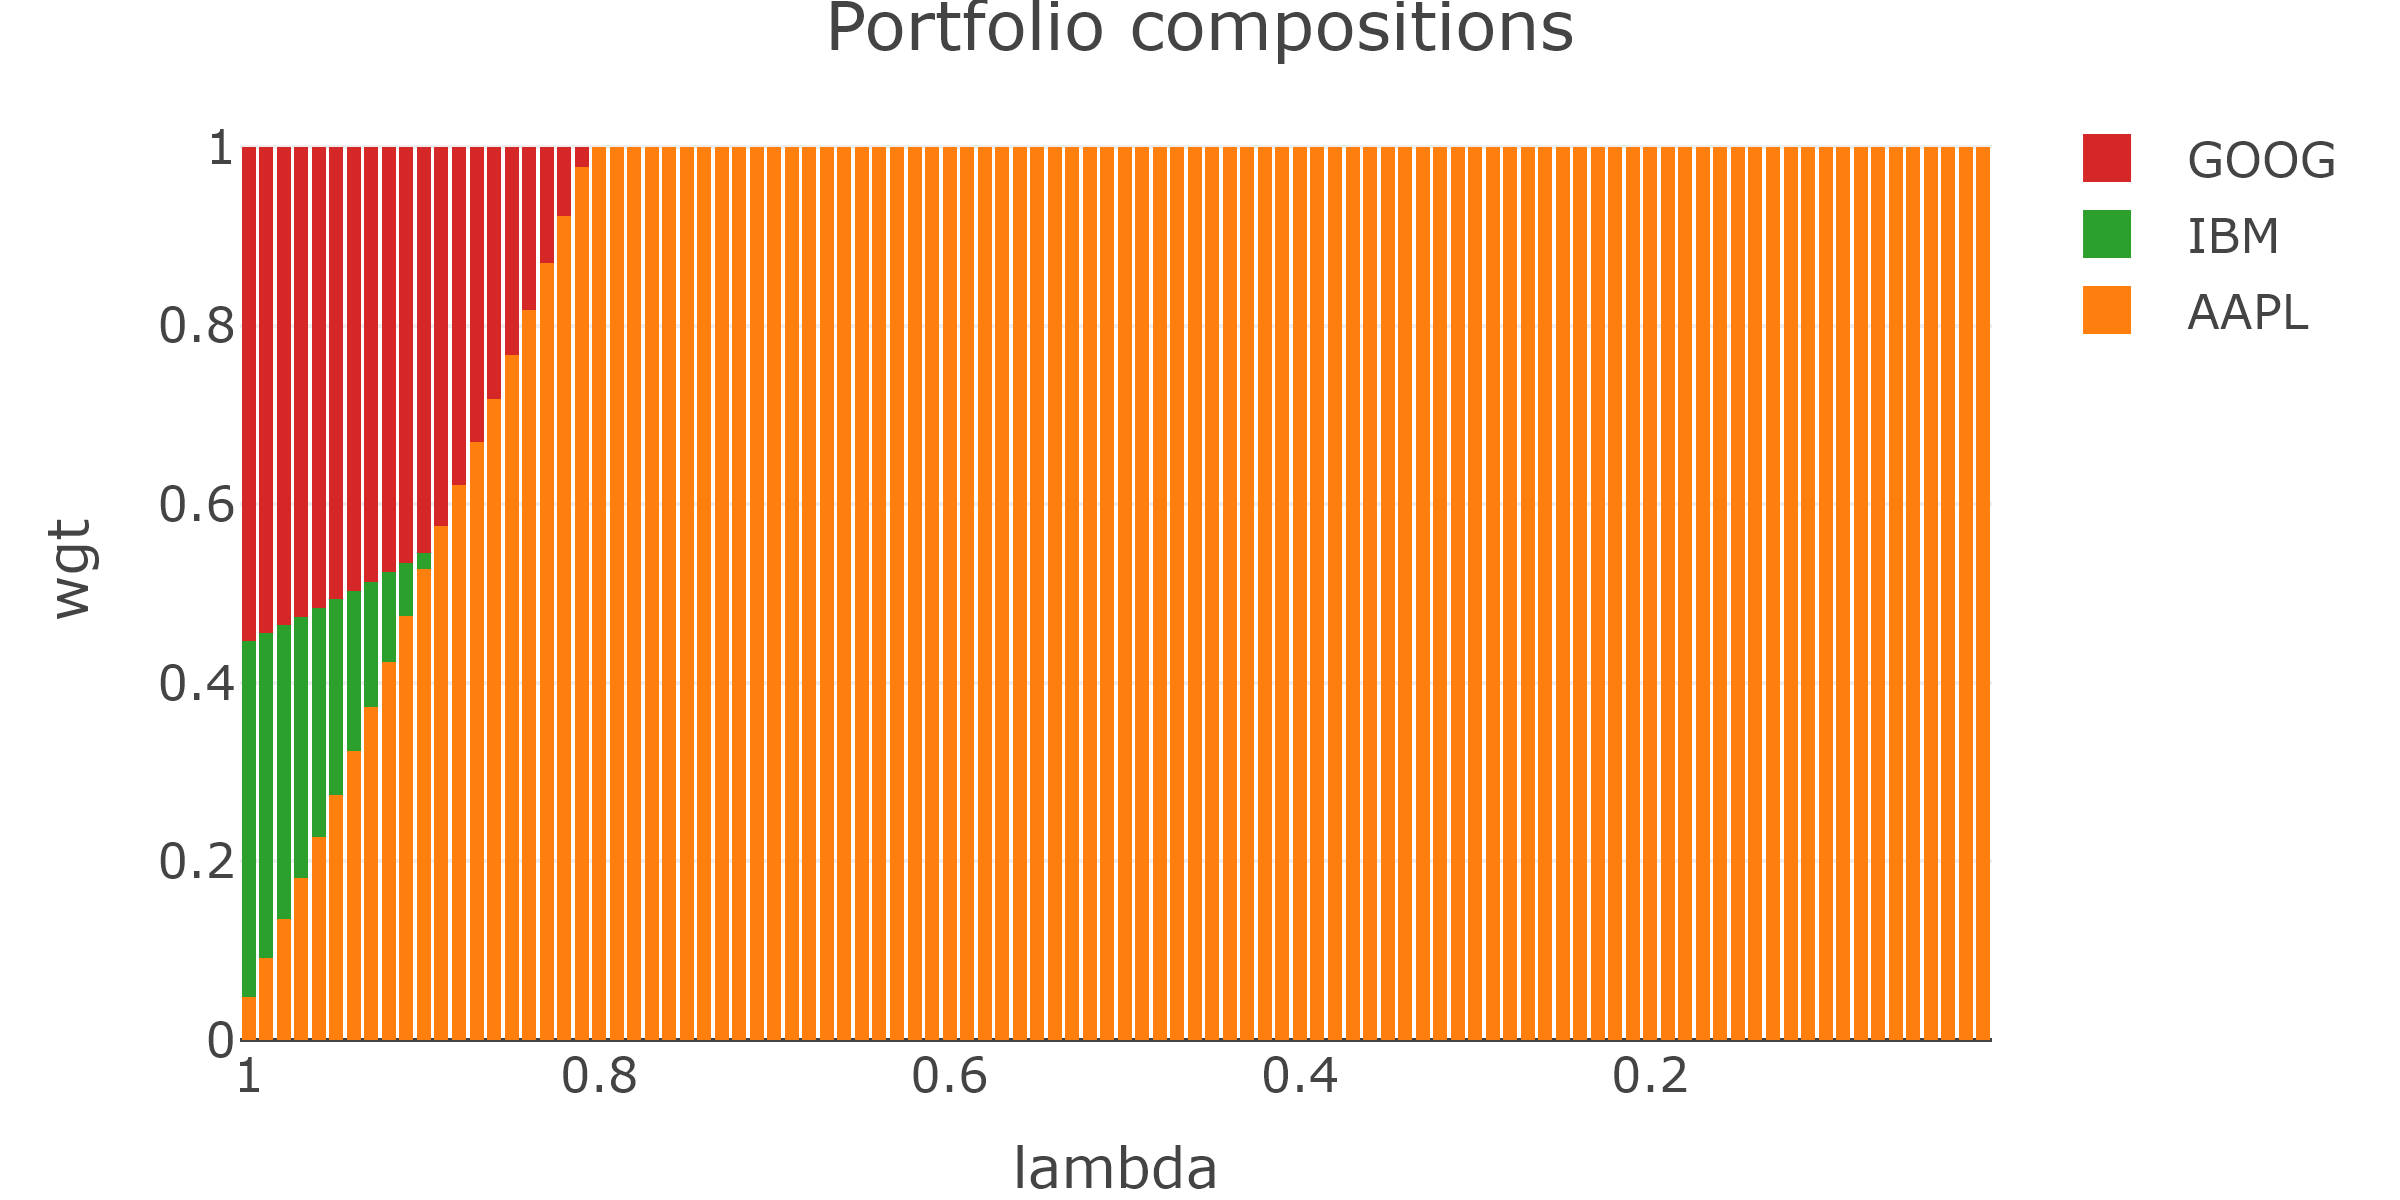
\includegraphics{Master_Thesis_files/figure-latex/unnamed-chunk-6-1} \caption{Comparison of the use of the arithmetic and geometric means in the calculation of MVP's for each lambda. The plot of MVP's in terms of mu - sigma is calculated with the arithmetic mean using the resulting portfolio weights}\label{fig:unnamed-chunk-6}
\end{figure}

It can be seen, that both estimators produce portfolios on the same efficient frontier. If the aim of the MVP is to generate a portfolio with minimal variance for a given return target, the type of return needs to be specified to use the geometric or arithmetic mean. This specification will determine the type of estimator needed for the MVP. This analogy is not needed in the scope of this thesis, because the more generic portfolios specified with \(\lambda\) are sufficient to create test-cases for the PSO. The later examples with the MVP will always use the geometric mean returns as estimation for the expected returns.

\hypertarget{index-tracking-portfolio-itp}{%
\section{Index-Tracking Portfolio (ITP)}\label{index-tracking-portfolio-itp}}

Indices are baskets of assets that are used to track the performance of a particular asset group. For example, the well-known Standard and Poor's 500 Index (abbreviated S\&P 500) tracks the 500 largest companies in the United States. Indices are not for sale and serve only to visualize the performance of a particular asset group, without incurring transaction costs. Such indices, or a combination of indices, are used by portfolio managers as benchmarks to compare the performance of their funds. Each fund has its own benchmark, which contains roughly the same assets that the manager might buy. If the fund underperforms its benchmark, it may indicate that the fund manager has made poor decisions. Therefore, fund managers strive to outperform their benchmarks through carefully selected investments. Past experience has shown that this is rarely achieved with active management by cost \citep{Desm2016}. This has led to the growing popularity of passively managed funds whose goal is to track their benchmarks as closely as possible. This can be achieved through either full or sparse replication. Full replication is a portfolio that contains all the assets in the benchmark with the same weightings. The resulting performance equals the performance of the benchmark when transaction costs are neglected. The first problem is that a benchmark may contain assets that are not liquid or cannot be purchased. The second problem is the weighting scheme of the indices, because they are often weighted by their market capitalization, which changes daily. This would result in the need to rebalance daily and increase transaction costs to replicate the performance of the benchmark as closely as possible. To avoid this, sparse replications are used that contain only a fraction of the benchmark's assets. To do so, the portfolio manager must define his benchmark, which serves as the investment universe for his fund. He then reduces this universe, taking into account investor constraints and availability, to create a pool of possible assets. For example, a pool that replicates the S\&P 500 might consist of the one hundred highest-weighted assets in the S\&P 500. The ITP can be modeled in two ways analysed in \citep{IuGa2019}.

\hypertarget{itpmste}{%
\subsection{ITP with TEV objective (ITP-TEV)}\label{itpmste}}

The classic and widely used model tries to reduce the tracking error variance (TEV) with the following formula:

\[
 \min \ \ Var(\pmb{TE}) = Var(\pmb{R}_{p}-\pmb{R}_{bm}),
\]

where the random tracking portfolio return is \(\pmb{R}_{p}\) and the random benchmark return is \(\pmb{R}_{bm}\). To obtain the portfolio weights \(w\), one needs to substitute the tracking portfolio return \(\pmb{R}_{p}\) as follows:

\[
  \pmb{R}_{p} = \pmb{R} \times w,
\]

where \(\pmb{R}\) is the random return vector containing the random return of each asset. The variance is then solved until a quadratic problem is presented as a function of portfolio weights \(w\):

\begin{align*}
 Var(\pmb{R}_{p}-\pmb{R}_{bm}) &= Var(\pmb{R} \times w - \pmb{R}_{bm}) \\
 &= Var(\pmb{R} \times w) + Var(\pmb{R}_{bm}) - 2 \cdot Cov(\pmb{R} \times w,\pmb{R}_{bm}).
\end{align*}

Now the three terms can be solved, starting with the simplest one.

\[
Var(\pmb{R}_{bm}) = \sigma_{bm}^2
\]

The variance of the portfolio can be solved with section \ref{portvar}:

\[
Var(\pmb{R} \times w) = w^T \times Cov(\pmb{R}) \times w.
\]

And the last term can be solved in the same way as in \citep{Eric2021}:

\begin{align*}
  Cov(\pmb{R} \times w, \pmb{R}_{bm}) &= Cov(\pmb{R}_{bm}, \pmb{R} \times w) \\
  &= E[(\pmb{R}_{bm}-\mu_{bm}) \cdot (\pmb{R} \times w-\mu_{\pmb{R}} \times w)] \\
  &= E[(\pmb{R}_{bm}-\mu_{bm}) \cdot (\pmb{R}-\mu_{\pmb{R}}) \times w] \\
  &= E[(\pmb{R}_{bm}-\mu_{bm}) \cdot (\pmb{R}-\mu_{\pmb{R}})] \times w \\
  &= Cov(\pmb{R}_{bm}, \pmb{R}) \times w.
\end{align*}

This results in the final formulation of the ITP:

\begin{align*}
  Var(\pmb{R}_{p}-\pmb{R}_{bm}) & = Var(\pmb{R} \times w - \pmb{R}_{bm}) \\
  & = Var(\pmb{R} \times w) - 2 \cdot Cov(\pmb{R} \times w,\pmb{R}_{bm}) + Var(\pmb{R}_{bm})  \\
  & = w^T \times Cov(\pmb{R}) \times w - 2 \cdot Cov(\pmb{R}_{bm}, \pmb{R}) \times w + \sigma_{bm}^2.
  \label{eq:ITP}
\end{align*}

The above problem can be estimated using the formulas and functions created in chapter \ref{mathfundations} and historical returns \(R\) and \(r_{bm}\). The minimization problem of the ITP in the general structure required by many optimizers is:

\[
  \min\limits_{w} \ \ \frac{1}{2} \cdot w^T \times D \times w -d^T \times w.
\]

Minimization problems can ignore constant terms and global stretch coefficients and still find the same minimum. This leads to a general substitution of the ITP with TEV objective as follows:

\[
  D = Cov(R)
\]

and

\[
d = Cov(r_{bm}, R)^T.
\]

It is possible to add some basic constraints, as in the MVP to sum the weights to 1 and be long only. Despite the fact that this model is often used, it has a big disadvantage in that it cannot detect constant deviations in the returns. For this reason, the following model exists, which focuses on the mean square tracking error of returns (MSTE).

\hypertarget{ITPMSTE}{%
\subsection{ITP with MSTE objective (ITP-MSTE)}\label{ITPMSTE}}

A good explanation of the ITP with MSTE objective can be found in \citep{AhBa2017}. The objective is to minimize the mean square tracking error (MSTE) of daily portfolio returns \(r_{t, p}\) and daily benchmark returns \(r_{t, bm}\) on \(T\) historical days:

\[
  \frac{1}{T} \sum^T_{t=1}(r_{t, p}-r_{t, bm})^2.
\]
The formula can be rewritten as vector norm:

\[
  \frac{1}{T} \left\Vert r_{p}-r_{bm} \right\Vert_2^2.
\]

This results in the following minimization with neglected stretching coefficient:

\[
 min \ \  \left\Vert r_{p}-r_{bm} \right\Vert_2^2.
\]

The portfolio returns \(r_p\) needs to be substituted to contain the portfolio weights \(w\) like in the TEV objective above. This results in the below transformation of the problem:

\begin{align*}
  \left\Vert r_{p}-r_{bm} \right\Vert_2^2 &= \left\Vert R \times w-r_{bm} \right\Vert_2^2 \\ 
  &= (R \times w-r_{bm})^T \times (R \times w-r_{bm}) \\ 
  &= (w^T \times R^T-r_{bm}^T) \times (R \times w-r_{bm}) \\ 
  &= w^T \times R^T \times R \times w - w^T \times R^T \times r_{bm} - r_{bm}^T \times R \times w + r_{bm}^T \times r_{bm}.
\end{align*}

The minimization and the fact that the scalars \(w^T \times R^T \times r_{bm}\) and \(r_{bm}^T \times R \times w\) are equal, transforms the problem to:

\[
  \min\limits_{w} \ \  \left\Vert r_{p}-r_{bm} \right\Vert_2^2 
  = w^T \times R^T \times R \times w - 2\cdot r_{bm}^T \times R \times w.
\]

This leads to the equivalent general representation of the ITP with MSTE objective as follows:

\[
  \min\limits_{w} \ \ \frac{1}{2} \cdot w^T \times D \times w - d^T \times w
\]

with

\[
D = R^T \times R
\]

and

\[
  d = R^T \times r_{bm}.
\]

\hypertarget{example-itp}{%
\subsection{Example ITP}\label{example-itp}}

This example shows the results of tracking the S\&P 500 with a tracking portfolio that can only invest in IBM, Apple and Google. Because the returns are calculated from adjusted closing prices, the index needs to represent dividends, stock splits and rights offerings too. This can be achieved by taking the S\&P 500 Total Return Index (abbreviated SP500TR). The time frame ranges from 2018-01-01 till 2019-12-31 and the goal is to minimize the difference in returns between the portfolio and the benchmark. The fitted performance of the ITP-TEV and ITP-MSTE are:

\begin{figure}[H]
\includegraphics{Master_Thesis_files/figure-latex/ITPex-1} \caption{Comparison of ITP-TEV and ITP-MSTE objectives, presented as cumulative daily returns}\label{fig:ITPex}
\end{figure}

The ITP-TEV and the ITP-MSTE produced almost the same results, which can be seen in the compositions below:

\vspace{0.1cm}\fontsize{11}{12}\selectfont

\begin{verbatim}
      type      AAPL       IBM      GOOG
1  ITP-TEV 0.2588843 0.4163274 0.3247883
2 ITP-MSTE 0.2586716 0.4165149 0.3248135
\end{verbatim}

\normalsize\vspace{0.1cm}

\hypertarget{analyticalsolver}{%
\chapter{Deterministic Optimization Methods for Quadratic Programming Problems}\label{analyticalsolver}}

\chaptermark{Deterministic Optimization Methods}

In this chapter, the advantages and disadvantages of deterministic optimization methods for quadratic programming problems are discussed. For simplicity, this thesis refers to the implementation of a deterministic optimization method as a solver. It is beyond the scope of this thesis to explain the underlying mathematical principles of how a solver handles quadratic problems; only the applications and analysis are discussed. The main reason for dealing with solvers for quadratic programming problems is to use them as a benchmark for the PSO.

\hypertarget{quadratic-programming-qp}{%
\section{Quadratic Programming (QP)}\label{quadratic-programming-qp}}

A quadratic program is a minimization problem of a function that returns a scalar and consists of a quadratic term and a linear term that depend on the variable of interest. In addition, the problem may be constrained by several linear inequalities that bound the solution. The general formulation used is to find \(x\) that minimizes the following problem:

\[
  \min\limits_{x} \ \frac{1}{2} \cdot x^T \times D \times x - d^T \times x 
\]

and is valid under the linear constraints:

\[
  A^T \times x \geq b_0.
\]

Some other sources notate the problem with different signs or coefficients, all of which are interchangeable with the above problem. In addition, the above problem has the same notation used in the R package \texttt{quadprog}, which reduces the substitution overhead. All modern programming languages have many solvers for quadratic problems. They differ mainly in the computation time for certain problems and the requirements. Some commercial QP solvers additionally accept more complex constraints, such as absolute (e.g., \(|A^T \times x| \geq a_0\)) or mixed-integer (e.g., \(x \in \mathbb{N}\)). Especially the mixed-integer constraint problems lead to a huge increase in memory requirements.

\hypertarget{qp-solver-from-quadprog}{%
\section{QP Solver from quadprog}\label{qp-solver-from-quadprog}}

The common free QP solver used in R comes from the package \href{https://cran.r-project.org/web/packages/quadprog/quadprog.pdf}{quadprog}, which consists of a single function called \texttt{solve.QP}. Its implementation routine is the dual method of Goldfarb and Idnani published in \citep{GoId1982} and \citep{GoId1983}. It uses the above QP with the condition that \(D\) must be a symmetric positive definite matrix. This means that \(D\in \mathbb{R}^{N \times N}\) and \(x^T D x > 0 \ \forall \ x \in \mathbb{R}^N \setminus \{\vec{0}\}\), which is equivalent to all eigenvalues being greater than zero. In most cases this is not achieved by estimating the covariance matrix \(\sum\), but it is possible to find the nearest positive definite matrix of \(\textstyle\sum\) using the function \texttt{nearPD()} from the \href{https://cran.r-project.org/web/packages/Matrix/Matrix.pdf}{matrix} R package. The error encountered often does not exceed a percent change in elements greater than \(10^{-15} \%\), which is negligible for the context of this work. The function \texttt{solve.QP} for an \(N\) dimensional vector of interest, has the following arguments, which are also found in the above formulation of a QP:

\begin{itemize}
\tightlist
\item
  \texttt{Dmat}: Symmetric positive definite matrix \(D \in \mathbb{R}^{N \times N}\) of the quadratic term
\item
  \texttt{dvec}: Vector \(d \in \mathbb{R}^{N}\) of the linear term
\item
  \texttt{Amat}: Constraint matrix \(A\)
\item
  \texttt{bvec}: Constraint vector \(b_0\)
\item
  \texttt{meq\ =\ 1}: means that the first \texttt{meq} columns of \(A\) are treated as an equality constraint
\end{itemize}

The return of \texttt{solve.QP} is a list and contains, among others, the following attributes of interest:

\begin{itemize}
\tightlist
\item
  \texttt{solution}: Vector containing the solution \(x\) of the quadratic programming problem (e.g.~portfolio weights)
\item
  \texttt{value}: Scalar, the value of the quadratic function at the solution
\end{itemize}

\hypertarget{exampleanalyticalmvp}{%
\section{\texorpdfstring{Solving MVP Problem with \texttt{solve.QP}}{Solving MVP Problem with solve.QP}}\label{exampleanalyticalmvp}}

This section provides insights into the effects of diversification and the use of \texttt{solve.QP} by creating ten different efficient frontiers from a pool of ten assets. Each efficient frontier \(i \in \{1, 2, \cdots, 10\}\) consists of \(N_i = i\) assets and is created by adding the asset with the next smallest variance first. After loading the returns for ten of the largest stocks in the U.S. market, the variance is calculated to rank all columns in ascending order of variance, as shown in the code below:

\vspace{0.1cm}\fontsize{11}{12}\selectfont

\begin{Shaded}
\begin{Highlighting}[]
\NormalTok{returns\_raw }\OtherTok{\textless{}{-}} \FunctionTok{buffer}\NormalTok{(}
  \FunctionTok{get\_yf}\NormalTok{(}
    \AttributeTok{tickers =} \FunctionTok{c}\NormalTok{(}\StringTok{"IBM"}\NormalTok{, }\StringTok{"GOOG"}\NormalTok{, }\StringTok{"AAPL"}\NormalTok{, }\StringTok{"MSFT"}\NormalTok{, }\StringTok{"AMZN"}\NormalTok{, }
                \StringTok{"NVDA"}\NormalTok{, }\StringTok{"JPM"}\NormalTok{, }\StringTok{"META"}\NormalTok{, }\StringTok{"V"}\NormalTok{, }\StringTok{"WMT"}\NormalTok{), }
    \AttributeTok{from =} \StringTok{"2018{-}01{-}01"}\NormalTok{, }
    \AttributeTok{to =} \StringTok{"2019{-}12{-}31"}
\NormalTok{  )}\SpecialCharTok{$}\NormalTok{returns, }
  \StringTok{"AS\_10\_assets"}
\NormalTok{)}

\CommentTok{\# re{-}arrange: low var first}
\NormalTok{vars }\OtherTok{\textless{}{-}} \FunctionTok{sapply}\NormalTok{(returns\_raw, var)}
\NormalTok{returns\_raw }\OtherTok{\textless{}{-}}\NormalTok{ returns\_raw[, }\FunctionTok{order}\NormalTok{(vars, }\AttributeTok{decreasing =}\NormalTok{ F)]}
\end{Highlighting}
\end{Shaded}

\normalsize\vspace{0.1cm}

The next step is to create a function \texttt{mvp()} that has the arguments \texttt{return} and \texttt{lambda}. It computes the expected returns \texttt{mu} and the estimated positive definite covariance \texttt{cov}. It then solves an MVP problem with constraints \(\textstyle\sum w_i = 1\) and \(w_i \geq 0\), which yields the key features \texttt{mu}, \texttt{var} and \texttt{composition} of the portfolio.

\vspace{0.1cm}\fontsize{11}{12}\selectfont

\begin{Shaded}
\begin{Highlighting}[]
\NormalTok{mvp }\OtherTok{\textless{}{-}} \ControlFlowTok{function}\NormalTok{(returns, lambda)\{}
\NormalTok{  tc }\OtherTok{\textless{}{-}} \FunctionTok{tryCatch}\NormalTok{(\{}
\NormalTok{    mu }\OtherTok{\textless{}{-}} \FunctionTok{ret\_to\_geomeanret}\NormalTok{(returns)}

\NormalTok{    cov }\OtherTok{\textless{}{-}} \FunctionTok{as.matrix}\NormalTok{(}\FunctionTok{nearPD}\NormalTok{(}\FunctionTok{cov\_}\NormalTok{(returns, mu))}\SpecialCharTok{$}\NormalTok{mat)}

\NormalTok{    mat }\OtherTok{\textless{}{-}} \FunctionTok{list}\NormalTok{(}
      \AttributeTok{Dmat =}\NormalTok{ lambda }\SpecialCharTok{*}\NormalTok{ cov,}
      \AttributeTok{dvec =}\NormalTok{ (}\DecValTok{1}\SpecialCharTok{{-}}\NormalTok{lambda) }\SpecialCharTok{*}\NormalTok{ mu,}
      \AttributeTok{Amat =} \FunctionTok{t}\NormalTok{(}\FunctionTok{rbind}\NormalTok{(}
        \FunctionTok{rep}\NormalTok{(}\DecValTok{1}\NormalTok{, }\FunctionTok{ncol}\NormalTok{(returns)), }\CommentTok{\# sum up to 1}
        \FunctionTok{diag}\NormalTok{(}
          \DecValTok{1}\NormalTok{, }\AttributeTok{nrow=}\FunctionTok{ncol}\NormalTok{(returns), }\AttributeTok{ncol=}\FunctionTok{ncol}\NormalTok{(returns)}
\NormalTok{        ) }\CommentTok{\# long only}
\NormalTok{      )),}
      \AttributeTok{bvec =} \FunctionTok{c}\NormalTok{(}
        \DecValTok{1}\NormalTok{, }\CommentTok{\# sum up to 1}
        \FunctionTok{rep}\NormalTok{(}\DecValTok{0}\NormalTok{, }\FunctionTok{ncol}\NormalTok{(returns)) }\CommentTok{\# long only}
\NormalTok{      ),}
      \AttributeTok{meq =} \DecValTok{1}
\NormalTok{    )}
  
\NormalTok{    qp }\OtherTok{\textless{}{-}} \FunctionTok{solve.QP}\NormalTok{(}
      \AttributeTok{Dmat =}\NormalTok{ mat}\SpecialCharTok{$}\NormalTok{Dmat, }\AttributeTok{dvec =}\NormalTok{ mat}\SpecialCharTok{$}\NormalTok{dvec, }
      \AttributeTok{Amat =}\NormalTok{ mat}\SpecialCharTok{$}\NormalTok{Amat, }\AttributeTok{bvec =}\NormalTok{ mat}\SpecialCharTok{$}\NormalTok{bvec, }\AttributeTok{meq =}\NormalTok{ mat}\SpecialCharTok{$}\NormalTok{meq}
\NormalTok{    )}
    
\NormalTok{    res }\OtherTok{\textless{}{-}} \FunctionTok{list}\NormalTok{(}
      \StringTok{"mu"} \OtherTok{=}\NormalTok{ mu }\SpecialCharTok{\%*\%}\NormalTok{ qp}\SpecialCharTok{$}\NormalTok{solution,}
      \StringTok{"var"} \OtherTok{=} \FunctionTok{t}\NormalTok{(qp}\SpecialCharTok{$}\NormalTok{solution) }\SpecialCharTok{\%*\%}\NormalTok{ cov }\SpecialCharTok{\%*\%}\NormalTok{ qp}\SpecialCharTok{$}\NormalTok{solution,}
      \StringTok{"composition"} \OtherTok{=} \FunctionTok{setNames}\NormalTok{(qp}\SpecialCharTok{$}\NormalTok{solution, }\FunctionTok{colnames}\NormalTok{(returns))}
\NormalTok{    )}
    \ConstantTok{TRUE}
\NormalTok{  \}, }\AttributeTok{error =} \ControlFlowTok{function}\NormalTok{(e)\{}\ConstantTok{FALSE}\NormalTok{\})}
  

  \ControlFlowTok{if}\NormalTok{(tc)\{}
    \FunctionTok{return}\NormalTok{(res)}
\NormalTok{  \}}\ControlFlowTok{else}\NormalTok{\{}
    \FunctionTok{return}\NormalTok{(}\FunctionTok{list}\NormalTok{(}
      \StringTok{"mu"} \OtherTok{=} \ConstantTok{NA}\NormalTok{,}
      \StringTok{"var"} \OtherTok{=} \ConstantTok{NA}\NormalTok{,}
      \StringTok{"composition"} \OtherTok{=} \ConstantTok{NA}
\NormalTok{    ))}
\NormalTok{  \}}
\NormalTok{\}}
\end{Highlighting}
\end{Shaded}

\normalsize\vspace{0.1cm}

Each \(\lambda \in \{0.01, 0.02, \cdots, 1\}\) and each combination of ascending number of assets results in a portfolio that can be created with two for loops.

\vspace{0.1cm}\fontsize{11}{12}\selectfont

\begin{Shaded}
\begin{Highlighting}[]
\NormalTok{df }\OtherTok{\textless{}{-}} \FunctionTok{data.frame}\NormalTok{(}
  \StringTok{"index"}\OtherTok{=}\DecValTok{1}\NormalTok{, }
  \StringTok{"var"}\OtherTok{=}\FunctionTok{as.numeric}\NormalTok{(}\FunctionTok{var}\NormalTok{(returns\_raw[, }\DecValTok{1}\NormalTok{])), }
  \StringTok{"return"} \OtherTok{=} \FunctionTok{as.numeric}\NormalTok{(}\FunctionTok{ret\_to\_geomeanret}\NormalTok{(returns\_raw[, }\DecValTok{1}\NormalTok{])), }
  \AttributeTok{row.names=}\ConstantTok{NULL}
\NormalTok{)}
\ControlFlowTok{for}\NormalTok{(i }\ControlFlowTok{in} \DecValTok{2}\SpecialCharTok{:}\FunctionTok{ncol}\NormalTok{(returns\_raw))\{}
\NormalTok{  returns }\OtherTok{\textless{}{-}}\NormalTok{ returns\_raw[, }\DecValTok{1}\SpecialCharTok{:}\NormalTok{i]}
  \ControlFlowTok{for}\NormalTok{(lambda }\ControlFlowTok{in} \FunctionTok{seq}\NormalTok{(}\FloatTok{0.01}\NormalTok{, }\DecValTok{1}\NormalTok{, }\FloatTok{0.01}\NormalTok{))\{}
\NormalTok{    res }\OtherTok{\textless{}{-}} \FunctionTok{mvp}\NormalTok{(returns, lambda)}
    
\NormalTok{    df }\OtherTok{\textless{}{-}} \FunctionTok{rbind}\NormalTok{(}
\NormalTok{      df, }
      \FunctionTok{data.frame}\NormalTok{(}\StringTok{"index"}\OtherTok{=}\NormalTok{i, }\StringTok{"var"}\OtherTok{=}\NormalTok{res}\SpecialCharTok{$}\NormalTok{var, }\StringTok{"return"} \OtherTok{=}\NormalTok{ res}\SpecialCharTok{$}\NormalTok{mu)}
\NormalTok{    )}
\NormalTok{  \}}
\NormalTok{\}}
\end{Highlighting}
\end{Shaded}

\normalsize\vspace{0.1cm}

The result is filtered and names are added to represent the number of assets. Now the \(\mu\)-\(\sigma\) diagram can be created:

\begin{figure}[H]
\includegraphics{Master_Thesis_files/figure-latex/qpmvp4-1} \caption{Comparison of efficiency frontiers generated from an ascending pool of assets, starting with the asset that has the lowest variance and sequentially adding the asset with the next lowest variance to the pool. Displayed in a mu - sigma diagramm}\label{fig:qpmvp4}
\end{figure}

It can be seen that each added asset leads to a minimum variance portfolio with a smaller or equal standard deviation. Despite starting with the asset that has the smallest standard deviation of 0.012459. This is the effect of diversification mentioned by Markowitz.

\hypertarget{exampleitpsolveqp}{%
\section{\texorpdfstring{Solving ITP-MSTE with \texttt{solve.QP}}{Solving ITP-MSTE with solve.QP}}\label{exampleitpsolveqp}}

This example analyzes how many assets are needed to minimize the mean square error between the replication and historical returns of the SP500TR from 2018-01-01 to 2019-12-31. The constraints are set to be long only and the weights should sum to one. To gradually reduce the number of assets, the five assets with the lowest weights are discarded, and the remaining assets serve as the new asset pool for the next replication until only five assets remain. First, the required data can be downloaded from the \texttt{R/} directory using existing functions. The function \texttt{get\_spx\_composition()} uses web scraping to read the components of \href{https://en.wikipedia.org/wiki/List_of_S\%26P_500_companies}{wikipedia} and converts them into monthly compositions of the SP500TR. The pool is formed from all assets present in the last month of the time frame, reduced by assets with missing values. The code below loads the returns of all assets in the pool and the SP500TR:

\vspace{0.1cm}\fontsize{11}{12}\selectfont

\begin{Shaded}
\begin{Highlighting}[]
\NormalTok{from }\OtherTok{\textless{}{-}} \StringTok{"2018{-}01{-}01"}
\NormalTok{to }\OtherTok{\textless{}{-}} \StringTok{"2019{-}12{-}31"}

\NormalTok{spx\_composition }\OtherTok{\textless{}{-}} \FunctionTok{buffer}\NormalTok{(}
  \FunctionTok{get\_spx\_composition}\NormalTok{(),}
  \StringTok{"AS\_spx\_composition"}
\NormalTok{)}


\NormalTok{pool\_returns\_raw }\OtherTok{\textless{}{-}} \FunctionTok{buffer}\NormalTok{(}
  \FunctionTok{get\_yf}\NormalTok{(}
    \AttributeTok{tickers =}\NormalTok{ spx\_composition }\SpecialCharTok{\%\textgreater{}\%} 
      \FunctionTok{filter}\NormalTok{(Date}\SpecialCharTok{\textless{}=}\NormalTok{to) }\SpecialCharTok{\%\textgreater{}\%} 
      \FunctionTok{filter}\NormalTok{(Date}\SpecialCharTok{==}\FunctionTok{max}\NormalTok{(Date)) }\SpecialCharTok{\%\textgreater{}\%} 
      \FunctionTok{pull}\NormalTok{(Ticker), }
    \AttributeTok{from =}\NormalTok{ from, }
    \AttributeTok{to =}\NormalTok{ to}
\NormalTok{  )}\SpecialCharTok{$}\NormalTok{returns, }
  \StringTok{"AS\_sp500\_assets"}
\NormalTok{)}
\NormalTok{pool\_returns\_raw }\OtherTok{\textless{}{-}} 
\NormalTok{  pool\_returns\_raw[, }\FunctionTok{colSums}\NormalTok{(}\FunctionTok{is.na}\NormalTok{(pool\_returns\_raw))}\SpecialCharTok{==}\DecValTok{0}\NormalTok{]}


\NormalTok{bm\_returns }\OtherTok{\textless{}{-}} \FunctionTok{buffer}\NormalTok{(}
  \FunctionTok{get\_yf}\NormalTok{(}\AttributeTok{tickers =} \StringTok{"\^{}SP500TR"}\NormalTok{, }\AttributeTok{from =}\NormalTok{ from, }\AttributeTok{to =}\NormalTok{ to)}\SpecialCharTok{$}\NormalTok{returns, }
  \StringTok{"AS\_sp500tr"}
\NormalTok{) }\SpecialCharTok{\%\textgreater{}\%} \FunctionTok{setNames}\NormalTok{(., }\StringTok{"SP500TR"}\NormalTok{)}
\end{Highlighting}
\end{Shaded}

\normalsize\vspace{0.1cm}

The required data is now available and the function for the ITP-MSTE can be created. It requires \texttt{pool\_returns} with variable number of columns and the single-column matrix \texttt{bm\_returns}.

\vspace{0.1cm}\fontsize{11}{12}\selectfont

\begin{Shaded}
\begin{Highlighting}[]
\NormalTok{itp }\OtherTok{\textless{}{-}} \ControlFlowTok{function}\NormalTok{(pool\_returns, bm\_returns)\{}
\NormalTok{  mat }\OtherTok{\textless{}{-}} \FunctionTok{list}\NormalTok{(}
    \AttributeTok{Dmat =} \FunctionTok{t}\NormalTok{(pool\_returns) }\SpecialCharTok{\%*\%}\NormalTok{ pool\_returns,}
    \AttributeTok{dvec =} \FunctionTok{t}\NormalTok{(pool\_returns) }\SpecialCharTok{\%*\%}\NormalTok{ bm\_returns,}
    \AttributeTok{Amat =} \FunctionTok{t}\NormalTok{(}\FunctionTok{rbind}\NormalTok{(}
      \FunctionTok{rep}\NormalTok{(}\DecValTok{1}\NormalTok{, }\FunctionTok{ncol}\NormalTok{(pool\_returns)), }\CommentTok{\# sum up to 1}
      \FunctionTok{diag}\NormalTok{(}\DecValTok{1}\NormalTok{, }
           \AttributeTok{nrow=}\FunctionTok{ncol}\NormalTok{(pool\_returns), }
           \AttributeTok{ncol=}\FunctionTok{ncol}\NormalTok{(pool\_returns)) }\CommentTok{\# long only}
\NormalTok{    )),}
    \AttributeTok{bvec =} \FunctionTok{c}\NormalTok{(}
      \DecValTok{1}\NormalTok{, }\CommentTok{\# sum up to 1}
      \FunctionTok{rep}\NormalTok{(}\DecValTok{0}\NormalTok{, }\FunctionTok{ncol}\NormalTok{(pool\_returns)) }\CommentTok{\# long only}
\NormalTok{    ),}
    \AttributeTok{meq =} \DecValTok{1}
\NormalTok{  )}
  
\NormalTok{  qp }\OtherTok{\textless{}{-}} \FunctionTok{solve.QP}\NormalTok{(}
    \AttributeTok{Dmat =}\NormalTok{ mat}\SpecialCharTok{$}\NormalTok{Dmat, }\AttributeTok{dvec =}\NormalTok{ mat}\SpecialCharTok{$}\NormalTok{dvec, }
    \AttributeTok{Amat =}\NormalTok{ mat}\SpecialCharTok{$}\NormalTok{Amat, }\AttributeTok{bvec =}\NormalTok{ mat}\SpecialCharTok{$}\NormalTok{bvec, }\AttributeTok{meq =}\NormalTok{ mat}\SpecialCharTok{$}\NormalTok{meq}
\NormalTok{  )}

\NormalTok{  res }\OtherTok{\textless{}{-}} \FunctionTok{list}\NormalTok{(}
    \StringTok{"var"} \OtherTok{=} \FunctionTok{as.numeric}\NormalTok{(}
      \FunctionTok{var}\NormalTok{(pool\_returns }\SpecialCharTok{\%*\%}\NormalTok{ qp}\SpecialCharTok{$}\NormalTok{solution }\SpecialCharTok{{-}}\NormalTok{ bm\_returns)),}
    \StringTok{"solution"} \OtherTok{=} \FunctionTok{setNames}\NormalTok{(qp}\SpecialCharTok{$}\NormalTok{solution, }\FunctionTok{colnames}\NormalTok{(pool\_returns))}
\NormalTok{  )}
\NormalTok{\}}
\end{Highlighting}
\end{Shaded}

\normalsize\vspace{0.1cm}

The successive removal of assets can begin and the results are stored in \texttt{res}.

\vspace{0.1cm}\fontsize{11}{12}\selectfont

\begin{Shaded}
\begin{Highlighting}[]
\NormalTok{res }\OtherTok{\textless{}{-}} \ConstantTok{NULL}
\NormalTok{asset\_pool }\OtherTok{\textless{}{-}} \ConstantTok{NULL}
\NormalTok{n\_assets }\OtherTok{\textless{}{-}} \FunctionTok{rev}\NormalTok{(}\FunctionTok{seq}\NormalTok{(}\DecValTok{5}\NormalTok{, }\FunctionTok{ncol}\NormalTok{(pool\_returns\_raw), }\DecValTok{5}\NormalTok{))}
\ControlFlowTok{for}\NormalTok{(i }\ControlFlowTok{in}\NormalTok{ n\_assets)\{}
\NormalTok{  temp }\OtherTok{\textless{}{-}} \ControlFlowTok{if}\NormalTok{(i}\SpecialCharTok{==}\FunctionTok{max}\NormalTok{(n\_assets))\{}
    \FunctionTok{itp}\NormalTok{(pool\_returns\_raw, bm\_returns)}
\NormalTok{  \}}\ControlFlowTok{else}\NormalTok{\{}
\NormalTok{    asset\_pool }\OtherTok{\textless{}{-}} \FunctionTok{names}\NormalTok{(}\FunctionTok{sort}\NormalTok{(temp}\SpecialCharTok{$}\NormalTok{solution, }\AttributeTok{decreasing =}\NormalTok{ T)[}\DecValTok{1}\SpecialCharTok{:}\NormalTok{i])}
    \FunctionTok{itp}\NormalTok{(}
\NormalTok{      pool\_returns\_raw[, asset\_pool], }
\NormalTok{      bm\_returns}
\NormalTok{    )}
\NormalTok{  \}}
\NormalTok{  res }\OtherTok{\textless{}{-}} \FunctionTok{rbind}\NormalTok{(}
\NormalTok{    res, }
    \FunctionTok{data.frame}\NormalTok{(}\StringTok{"N"}\OtherTok{=}\NormalTok{i, }\StringTok{"var"}\OtherTok{=}\NormalTok{temp}\SpecialCharTok{$}\NormalTok{var, }\StringTok{"sd"}\OtherTok{=}\FunctionTok{sqrt}\NormalTok{(temp}\SpecialCharTok{$}\NormalTok{var), }\AttributeTok{row.names =} \ConstantTok{NULL}\NormalTok{)}
\NormalTok{  )}
  
  \CommentTok{\# for later analysis}
  \ControlFlowTok{if}\NormalTok{(}\FunctionTok{length}\NormalTok{(asset\_pool)}\SpecialCharTok{==}\DecValTok{100}\NormalTok{)\{}
\NormalTok{    assets\_pool\_100 }\OtherTok{\textless{}{-}}\NormalTok{ asset\_pool}
    \FunctionTok{save}\NormalTok{(assets\_pool\_100, }\AttributeTok{file=}\StringTok{"data/assets\_pool\_100.rdata"}\NormalTok{)}
\NormalTok{  \}}
  \ControlFlowTok{if}\NormalTok{(}\FunctionTok{length}\NormalTok{(asset\_pool)}\SpecialCharTok{==}\DecValTok{50}\NormalTok{)\{}
\NormalTok{    assets\_pool\_50 }\OtherTok{\textless{}{-}}\NormalTok{ asset\_pool}
    \FunctionTok{save}\NormalTok{(assets\_pool\_50, }\AttributeTok{file=}\StringTok{"data/assets\_pool\_50.rdata"}\NormalTok{)}
\NormalTok{  \}}
\NormalTok{\}}
\end{Highlighting}
\end{Shaded}

\normalsize\vspace{0.1cm}

The following chart illustrates the increase in standard deviation to track the historical performance of the SP500TR as the number of assets \(N\) in the asset pool decreases:

\begin{figure}[H]
\includegraphics{Master_Thesis_files/figure-latex/qpitp4-1} \caption{Standard deviation between the performance of the SP500TR and the tracking portfolio over the fitting period for each asset pool of size N. The asset pool was created successively by discarding the five assets with the lowest weights to create the next pool}\label{fig:qpitp4}
\end{figure}

It can be seen that the standard deviation stagnates at about \(N=200\). This leads to the conclusion that a sparse replication with two hundred assets is sufficient in this particular case to track the historical performance of the SP500TR over this period.

\hypertarget{spso}{%
\chapter{Particle Swarm Optimization}\label{spso}}

The PSO was developed by J. Kennedy as a global optimization method based on swarm intelligence and presented to the public in 1995 by Eberhart and Kennedy \citep{KeEb1995}. The original PSO was intended to resemble a flock of birds flying through the sky without collisions. Therefore, its first applications were found in particle physics to analyze moving particles in high-dimensional spaces, which the name Particle recalls. Later, it was adapted in Evolutionary Computation to exploit a set of potential solutions in high dimensions and to find the optima by cooperating with other particles in the swarm \citep{PaVr2002}. Since it does not require gradient information, it is easier to apply than other global optimization methods. It can find the optimum by considering only the result of the function to be optimized. This means that the function can be arbitrarily complex and it is still possible to reach the global optimum. Other advantages are extensibility, simplicity, and low computational cost, since only basic mathematical operators are used.

\hypertarget{the-algorithm}{%
\section{The Algorithm}\label{the-algorithm}}

Each particle \(d\) with position \(x_d\) moves in the search space \(\mathbb{R}^N\) and has its own velocity \(v_d\) and remembers its previous best position \(p_{p,d}\). After each iteration, the velocity changes in the direction of the intrinsic velocity, the best previous position, and the global best position \(p_g\) of all particles. A position change from \(i\) to \(i+1\) can be calculated by the following two equations \citep{PaVr2002}:

\[
\begin{aligned}
  v_d^{i+1} &= wv_d^{i} + c_p r_1^{i(d)} (p_{p,d}^i - x_d^i) + c_g r_2^{i(d)} (p_g^i - x_d^i) \\
  x_d^{i+1} &= x_d^i + v_d^{i+1}.
\end{aligned}
\]

Where \(r_1^{i(d)}\) and \(r_2^{i(d)}\) are uniformly distributed random numbers in \([0, 1]\). The cognitive parameter \(c_p\) acts as a weighting of the direction to its previous best position of the particle. This contrasts with the social parameter \(c_g\), which is a weighting of the direction to the global best position. The inertia weight \(w\) is crucial for the convergence behavior by remembering part of its previous trajectory. A study reviewed in \citep{PaVr2002} showed that these parameters can be set to \(c_p=c_g=0.5\) and \(w\) should decrease from \(1.2\) to \(0\). However, some problems benefit from a more precise tuning of these parameters. To allow effortless translation to code, the above formula for \(d = 1, 2, \cdots, D\) particles can be given in the following matrix notation:

\[
\begin{aligned}
  V^{i+1} &= w \cdot V^{i} + c_p \cdot (\vec{r}_1^{\,i} \cdot (P^i-X^i)^T)^T + c_g \cdot (\vec{r}_2^{\,i} \cdot (p_g^i - X^i)^T)^T \\
  X^{i+1} &= X^i + V^{i+1}
\end{aligned}
\]

with current positions \(X \in \mathbb{R}^{N \times D}\), current velocities \(V \in \mathbb{R}^{N \times D}\), previous best positions \(P \in \mathbb{R}^{N \times D}\), and global best position \(p_g \in \mathbb{R}^{N}\). The parameters \(w\), \(c_p\) and \(c_g\) are stile scalars. The random numbers \(r_1\) and \(r_2\) are replaced by the vectors \(\vec{r}_1\) and \(\vec{r}_2\), in which each element is a uniformly distributed random number generated in \([0, 1]\). The first transpose is needed to multiply each random number element-wise with each column and the second transpose transforms it back to the format of \(V\) and \(X\).

The algorithm mentioned above is the first published variant of PSO and is therefore referred to as standard PSO in this thesis. There are also other names like global PSO, because the information is distributed globally over all particles in the swarm and some also call it the basic or original PSO.

\hypertarget{pso-function}{%
\section{\texorpdfstring{\texttt{pso()} Function}{pso() Function}}\label{pso-function}}

In this section, a general PSO function is created that follows the structure of other optimization heuristics in R, in particular the existing PSO implementation from the R package \texttt{pso}. The key component of the problem is a objective function called \texttt{fn()}, which needs a vector that describes the position of one particle (e.g.~weights) and returns a scalar that needs to be minimized. The other main parameter for the PSO function is \texttt{par}, which is a position of a particle used to derive the dimension of the problem and used as the initial position of one particle. The vector can contain only \texttt{NA}'s, resulting in completely random starting positions. The last two arguments are \texttt{lower} and \texttt{upper} bounds (e.g.~weights greater than 0 and less than 1). All other parameters have default values that can be overridden by passing a list called \texttt{control}. The resulting structure is:

\vspace{0.1cm}\fontsize{11}{12}\selectfont

\begin{Shaded}
\begin{Highlighting}[]
\NormalTok{pso }\OtherTok{\textless{}{-}} \ControlFlowTok{function}\NormalTok{(}
\NormalTok{    par, }
\NormalTok{    fn, }
\NormalTok{    lower, }
\NormalTok{    upper, }
    \AttributeTok{control =} \FunctionTok{list}\NormalTok{()}
\NormalTok{  )\{\}}
\end{Highlighting}
\end{Shaded}

\normalsize\vspace{0.1cm}

Before the main data structure can be initialized, some sample inputs must be created for the \texttt{pso()} function as described below:

\vspace{0.1cm}\fontsize{11}{12}\selectfont

\begin{Shaded}
\begin{Highlighting}[]
\NormalTok{par }\OtherTok{\textless{}{-}} \FunctionTok{rep}\NormalTok{(}\ConstantTok{NA}\NormalTok{, }\DecValTok{2}\NormalTok{)}
\NormalTok{fn }\OtherTok{\textless{}{-}} \ControlFlowTok{function}\NormalTok{(x)\{}\FunctionTok{return}\NormalTok{(}\FunctionTok{sum}\NormalTok{(}\FunctionTok{abs}\NormalTok{(x)))\}}
\NormalTok{lower }\OtherTok{\textless{}{-}} \SpecialCharTok{{-}}\DecValTok{10}
\NormalTok{upper }\OtherTok{\textless{}{-}} \DecValTok{10}
\NormalTok{control }\OtherTok{=} \FunctionTok{list}\NormalTok{(}
  \AttributeTok{s =} \DecValTok{10}\NormalTok{, }\CommentTok{\# swarm size}
  \AttributeTok{c.p =} \FloatTok{0.5}\NormalTok{, }\CommentTok{\# inherit best}
  \AttributeTok{c.g =} \FloatTok{0.5}\NormalTok{, }\CommentTok{\# global best}
  \AttributeTok{maxiter =} \DecValTok{100}\NormalTok{, }\CommentTok{\# iterations}
  \AttributeTok{w0 =} \FloatTok{1.2}\NormalTok{, }\CommentTok{\# starting inertia weight}
  \AttributeTok{wN =} \DecValTok{0}\NormalTok{, }\CommentTok{\# ending inertia weight}
  \AttributeTok{save\_traces =}\NormalTok{ F }\CommentTok{\# save more information}
\NormalTok{)}
\end{Highlighting}
\end{Shaded}

\normalsize\vspace{0.1cm}

Now it is time to initialize the random positions \texttt{X}, their fitness \texttt{X\_fit} and their random velocities \texttt{V} with the created function \texttt{mrunif()} which produces a matrix of uniformly distributed random numbers between \texttt{lower} and \texttt{upper}:

\vspace{0.1cm}\fontsize{11}{12}\selectfont

\begin{Shaded}
\begin{Highlighting}[]
\FunctionTok{set.seed}\NormalTok{(}\DecValTok{0}\NormalTok{)}
\NormalTok{X }\OtherTok{\textless{}{-}} \FunctionTok{mrunif}\NormalTok{(}
  \AttributeTok{nr =} \FunctionTok{length}\NormalTok{(par), }\AttributeTok{nc=}\NormalTok{control}\SpecialCharTok{$}\NormalTok{s, }\AttributeTok{lower=}\NormalTok{lower, }\AttributeTok{upper=}\NormalTok{upper}
\NormalTok{)}
\ControlFlowTok{if}\NormalTok{(}\FunctionTok{all}\NormalTok{(}\SpecialCharTok{!}\FunctionTok{is.na}\NormalTok{(par)))\{}
\NormalTok{  X[, }\DecValTok{1}\NormalTok{] }\OtherTok{\textless{}{-}}\NormalTok{ par}
\NormalTok{\}}
\NormalTok{X\_fit }\OtherTok{\textless{}{-}} \FunctionTok{apply}\NormalTok{(X, }\DecValTok{2}\NormalTok{, fn)}
\NormalTok{V }\OtherTok{\textless{}{-}} \FunctionTok{mrunif}\NormalTok{(}
  \AttributeTok{nr =} \FunctionTok{length}\NormalTok{(par), }\AttributeTok{nc=}\NormalTok{control}\SpecialCharTok{$}\NormalTok{s, }
  \AttributeTok{lower=}\SpecialCharTok{{-}}\NormalTok{(upper}\SpecialCharTok{{-}}\NormalTok{lower), }\AttributeTok{upper=}\NormalTok{(upper}\SpecialCharTok{{-}}\NormalTok{lower)}
\NormalTok{)}\SpecialCharTok{/}\DecValTok{10}
\end{Highlighting}
\end{Shaded}

\normalsize\vspace{0.1cm}

The velocities are compressed by a factor of 10 to start with a maximum movement of one tenth of the space in each axis. The personal best positions \texttt{P} are the same as \texttt{X} and the global best position is the position with the smallest fitness:

\vspace{0.1cm}\fontsize{11}{12}\selectfont

\begin{Shaded}
\begin{Highlighting}[]
\NormalTok{P }\OtherTok{\textless{}{-}}\NormalTok{ X}
\NormalTok{P\_fit }\OtherTok{\textless{}{-}}\NormalTok{ X\_fit}
\NormalTok{p\_g }\OtherTok{\textless{}{-}}\NormalTok{ P[, }\FunctionTok{which.min}\NormalTok{(P\_fit)]}
\NormalTok{p\_g\_fit }\OtherTok{\textless{}{-}} \FunctionTok{min}\NormalTok{(P\_fit)}
\end{Highlighting}
\end{Shaded}

\normalsize\vspace{0.1cm}

The required data structure is available and the optimization can start with the calculation of the new velocities and the transformation of the old positions. When particles have left the valid space of an axis, they are pushed back to the edge and the velocity on this axis is set to zero. Then the fitness is calculated and the personal best and global best positions are saved if they have improved.

\vspace{0.1cm}\fontsize{11}{12}\selectfont

\begin{Shaded}
\begin{Highlighting}[]
\NormalTok{trace\_data }\OtherTok{\textless{}{-}} \ConstantTok{NULL}
\ControlFlowTok{for}\NormalTok{(i }\ControlFlowTok{in} \DecValTok{1}\SpecialCharTok{:}\NormalTok{control}\SpecialCharTok{$}\NormalTok{maxiter)\{}
  \CommentTok{\# move particles}
\NormalTok{  V }\OtherTok{\textless{}{-}} 
\NormalTok{    (control}\SpecialCharTok{$}\NormalTok{w0}\SpecialCharTok{{-}}\NormalTok{(control}\SpecialCharTok{$}\NormalTok{w0}\SpecialCharTok{{-}}\NormalTok{control}\SpecialCharTok{$}\NormalTok{wN)}\SpecialCharTok{*}\NormalTok{i}\SpecialCharTok{/}\NormalTok{control}\SpecialCharTok{$}\NormalTok{maxiter) }\SpecialCharTok{*}\NormalTok{ V }\SpecialCharTok{+} 
\NormalTok{      control}\SpecialCharTok{$}\NormalTok{c.p }\SpecialCharTok{*} \FunctionTok{t}\NormalTok{(}\FunctionTok{runif}\NormalTok{(}\FunctionTok{ncol}\NormalTok{(X)) }\SpecialCharTok{*} \FunctionTok{t}\NormalTok{(P}\SpecialCharTok{{-}}\NormalTok{X)) }\SpecialCharTok{+}
\NormalTok{      control}\SpecialCharTok{$}\NormalTok{c.g }\SpecialCharTok{*} \FunctionTok{t}\NormalTok{(}\FunctionTok{runif}\NormalTok{(}\FunctionTok{ncol}\NormalTok{(X)) }\SpecialCharTok{*} \FunctionTok{t}\NormalTok{(p\_g}\SpecialCharTok{{-}}\NormalTok{X))}
\NormalTok{  X }\OtherTok{\textless{}{-}}\NormalTok{ X }\SpecialCharTok{+}\NormalTok{ V}
  
  \CommentTok{\# set velocity to zeros if not in valid space}
\NormalTok{  V[X }\SpecialCharTok{\textgreater{}}\NormalTok{ upper] }\OtherTok{\textless{}{-}} \DecValTok{0}
\NormalTok{  V[X }\SpecialCharTok{\textless{}}\NormalTok{ lower] }\OtherTok{\textless{}{-}} \DecValTok{0}
  
  \CommentTok{\# move into valid space}
\NormalTok{  X[X }\SpecialCharTok{\textgreater{}}\NormalTok{ upper] }\OtherTok{\textless{}{-}}\NormalTok{ upper}
\NormalTok{  X[X }\SpecialCharTok{\textless{}}\NormalTok{ lower] }\OtherTok{\textless{}{-}}\NormalTok{ lower}
  
  \CommentTok{\# evaluate objective function}
\NormalTok{  X\_fit }\OtherTok{\textless{}{-}} \FunctionTok{apply}\NormalTok{(X, }\DecValTok{2}\NormalTok{, fn)}
  
  \CommentTok{\# save new previews best}
\NormalTok{  P[, P\_fit }\SpecialCharTok{\textgreater{}}\NormalTok{ X\_fit] }\OtherTok{\textless{}{-}}\NormalTok{ X[, P\_fit }\SpecialCharTok{\textgreater{}}\NormalTok{ X\_fit]}
\NormalTok{  P\_fit[P\_fit }\SpecialCharTok{\textgreater{}}\NormalTok{ X\_fit] }\OtherTok{\textless{}{-}}\NormalTok{ X\_fit[P\_fit }\SpecialCharTok{\textgreater{}}\NormalTok{ X\_fit]}

  \CommentTok{\# save new global best}
  \ControlFlowTok{if}\NormalTok{(}\FunctionTok{any}\NormalTok{(P\_fit }\SpecialCharTok{\textless{}}\NormalTok{ p\_g\_fit))\{}
\NormalTok{    p\_g }\OtherTok{\textless{}{-}}\NormalTok{ P[, }\FunctionTok{which.min}\NormalTok{(P\_fit)]}
\NormalTok{    p\_g\_fit }\OtherTok{\textless{}{-}} \FunctionTok{min}\NormalTok{(P\_fit)}
\NormalTok{  \}}
\NormalTok{\}}
\end{Highlighting}
\end{Shaded}

\normalsize\vspace{0.1cm}

The global minimum is located at \([0, 0]\) which has a fitness of \(0\) and the best position found from the PSO after \(100\) iterations is located at {[}0.000007596889, 0.000001662703{]} and has a fitness of 0.0000093.

\hypertarget{animation-2-dimensional}{%
\section{Animation 2-Dimensional}\label{animation-2-dimensional}}

This section provides insights into the behavior of the PSO by visualizing multiple iterations in a GIF. The GIF works in Adobe Acrobat DC or in the Markdown/HTML version of this thesis. The animation template and the objective function is inspired by \citep{Rtic2021}. The PSO core from the above chapter was used to complete the \texttt{pso()} function and is tested here with seed 0. The objective is to minimize the following function (\(f:\mathbb{R}^2 \rightarrow \mathbb{R}\)):

\[
f(x, y) = -20\cdot e^{-0.2 \cdot \sqrt{0.5 \cdot ((x-1)^2 + (y-1)^2)}} \ - e^{0.5 \cdot ( cos(2\cdot \pi \cdot x) + cos(2\cdot \pi \cdot y))} + e + 20.
\]

The following code runs the PSO and tries to minimize the objective function:

\vspace{0.1cm}\fontsize{11}{12}\selectfont

\begin{Shaded}
\begin{Highlighting}[]
\FunctionTok{set.seed}\NormalTok{(}\DecValTok{0}\NormalTok{)}

\NormalTok{f }\OtherTok{\textless{}{-}} \ControlFlowTok{function}\NormalTok{(pos)\{}
  \SpecialCharTok{{-}}\DecValTok{20} \SpecialCharTok{*} \FunctionTok{exp}\NormalTok{(}\SpecialCharTok{{-}}\FloatTok{0.2} \SpecialCharTok{*} \FunctionTok{sqrt}\NormalTok{(}\FloatTok{0.5} \SpecialCharTok{*}\NormalTok{((pos[}\DecValTok{1}\NormalTok{]}\SpecialCharTok{{-}}\DecValTok{1}\NormalTok{)}\SpecialCharTok{\^{}}\DecValTok{2} \SpecialCharTok{+}\NormalTok{ (pos[}\DecValTok{2}\NormalTok{]}\SpecialCharTok{{-}}\DecValTok{1}\NormalTok{)}\SpecialCharTok{\^{}}\DecValTok{2}\NormalTok{))) }\SpecialCharTok{{-}} 
  \FunctionTok{exp}\NormalTok{(}\FloatTok{0.5}\SpecialCharTok{*}\NormalTok{(}\FunctionTok{cos}\NormalTok{(}\DecValTok{2}\SpecialCharTok{*}\NormalTok{pi}\SpecialCharTok{*}\NormalTok{pos[}\DecValTok{1}\NormalTok{]) }\SpecialCharTok{+} \FunctionTok{cos}\NormalTok{(}\DecValTok{2}\SpecialCharTok{*}\NormalTok{pi}\SpecialCharTok{*}\NormalTok{pos[}\DecValTok{2}\NormalTok{]))) }\SpecialCharTok{+} 
  \FunctionTok{exp}\NormalTok{(}\DecValTok{1}\NormalTok{) }\SpecialCharTok{+} \DecValTok{20}
\NormalTok{\}}

\NormalTok{res }\OtherTok{\textless{}{-}} \FunctionTok{pso}\NormalTok{(}
  \AttributeTok{par =} \FunctionTok{rep}\NormalTok{(}\ConstantTok{NA}\NormalTok{, }\DecValTok{2}\NormalTok{),}
  \AttributeTok{fn =}\NormalTok{ f,}
  \AttributeTok{lower =} \SpecialCharTok{{-}}\DecValTok{10}\NormalTok{,}
  \AttributeTok{upper =} \DecValTok{10}\NormalTok{,}
  \AttributeTok{control =} \FunctionTok{list}\NormalTok{(}
    \AttributeTok{s =} \DecValTok{10}\NormalTok{,}
    \AttributeTok{maxiter =} \DecValTok{30}\NormalTok{,}
    \AttributeTok{w0 =} \FloatTok{1.2}\NormalTok{,}
    \AttributeTok{save\_traces =}\NormalTok{ T}
\NormalTok{  )}
\NormalTok{)}
\end{Highlighting}
\end{Shaded}

\normalsize\vspace{0.1cm}

The function \texttt{f} has many local minima and a global minimum at \((1,1)\) with the value \(0\). The background color scale ranges from 0 as purple to 20 as yellow. The PSO has 10 particles, iterated 30 times with an inertia weight decreasing from 0.8 to 0. The iterations are visualized in the following GIF:

\begin{center}
\animategraphics[loop, width=10cm]{5}{./gifs/pso_2dim_v2/gif_2dim_}{1}{40}
\begin{figure}[!h]
\caption{Visualization of the behavior of the standard PSO in a GIF.}
\end{figure}
\end{center}

\hypertarget{animation-2-dimensional-app}{%
\section{Animation 2-Dimensional App}\label{animation-2-dimensional-app}}

To gain an even better understanding of the behavior of a PSO, a WebApp was developed that allows the user to minimize any two-dimensional functions with constraints. Three variants of the PSO were implemented, which will be analyzed in detail in the later chapters of this thesis. The app can also be used to study the effect of hyperparameters on the behavior of the PSO in more detail. Within the app it is possible to display each step of the iterations and this even with all the direction vectors that generate the resulting motion of each particle. The app is hosted at \citep{PSOApp} and the code for it is also freely available at \citep{GitPSO}. The hosted app may be used for educational purposes and using, copying, modifying, and sharing the code is permitted without restriction.

\hypertarget{simple-constraint-handling}{%
\section{Simple Constraint Handling}\label{simple-constraint-handling}}

The simplest method for dealing with constraints is the penalty method, which takes into account the intensity of constraint breaks by increasing the objective value of a minimization problem. The two common problems studied in the last two chapters are quadratic problems with the same structure of constraints. This can be used to create a generic constraint handling function for these particular QP's. Both problems must satisfy the following equation:

\[
  A^T \times x  \geq b_0
\]

To calculate a value for the intensity of constraint breaks, the above inequality is subtracted by \(b_0\) and the left-hand side is defined as follows:

\[
  c := A^T \times x - b_0.
\]

All negative elements in the vector \(c\) represent constraint breaks that are squared and summed to extract a value that describes the intensity of constraint breaks like follows:

\[
  c_{break} = \sum p(c_i)^2
\]

with

\[
 p(x) =   \begin{cases}
  0 &\text{ if }x \geq 0\\
  x &\text{ if }x < 0.
  \end{cases}
\]

By following the name conventions of \texttt{solve.QP}, a list named \texttt{mat} is created in the parent environment, that contains the necessary inputs. The generic R function to calculate the constraint breaks can be defined as follows:

\vspace{0.1cm}\fontsize{11}{12}\selectfont

\begin{Shaded}
\begin{Highlighting}[]
\NormalTok{calc\_const }\OtherTok{\textless{}{-}} \ControlFlowTok{function}\NormalTok{(x)\{}
\NormalTok{  const }\OtherTok{\textless{}{-}} \FunctionTok{t}\NormalTok{(mat}\SpecialCharTok{$}\NormalTok{Amat) }\SpecialCharTok{\%*\%}\NormalTok{ x }\SpecialCharTok{{-}}\NormalTok{ mat}\SpecialCharTok{$}\NormalTok{bvec}
  \FunctionTok{sum}\NormalTok{(}\FunctionTok{pmin}\NormalTok{(}\DecValTok{0}\NormalTok{, const)}\SpecialCharTok{\^{}}\DecValTok{2}\NormalTok{)}
\NormalTok{\}}
\end{Highlighting}
\end{Shaded}

\normalsize\vspace{0.1cm}

In contrast to the \texttt{solve.QP}, it's difficult for the PSO to find a feasible point, if equality constraints are used, which is why the equality constraint \(\textstyle\sum w_i = 1\) is reduced to \(0.99 \leq \textstyle\sum w_i\) and \(\textstyle\sum w_i \leq 1\).

The new objective function \texttt{fn()} consists of two parts. The first part is to evaluate the unconstrained objective of the QP with the following function:

\vspace{0.1cm}\fontsize{11}{12}\selectfont

\begin{Shaded}
\begin{Highlighting}[]
\NormalTok{calc\_fit }\OtherTok{\textless{}{-}} \ControlFlowTok{function}\NormalTok{(x)\{}
  \FloatTok{0.5} \SpecialCharTok{*} \FunctionTok{t}\NormalTok{(x) }\SpecialCharTok{\%*\%}\NormalTok{ mat}\SpecialCharTok{$}\NormalTok{Dmat }\SpecialCharTok{\%*\%}\NormalTok{ x }\SpecialCharTok{{-}} \FunctionTok{t}\NormalTok{(mat}\SpecialCharTok{$}\NormalTok{dvec) }\SpecialCharTok{\%*\%}\NormalTok{ x}
\NormalTok{\}}
\end{Highlighting}
\end{Shaded}

\normalsize\vspace{0.1cm}

The second part is the function \texttt{calc\_const()}. Since breaking constraints is much worse than losing fitness, it must have a higher intensity (e.g.~10) which must be fine-tuned. This results in the final \texttt{fn()} function composition:

\vspace{0.1cm}\fontsize{11}{12}\selectfont

\begin{Shaded}
\begin{Highlighting}[]
\NormalTok{fn }\OtherTok{\textless{}{-}} \ControlFlowTok{function}\NormalTok{(x)\{}
\NormalTok{  fitness }\OtherTok{\textless{}{-}} \FunctionTok{calc\_fit}\NormalTok{(x)}
\NormalTok{  constraints }\OtherTok{\textless{}{-}} \FunctionTok{calc\_const}\NormalTok{(x)}
  \FunctionTok{return}\NormalTok{(fitness }\SpecialCharTok{+} \DecValTok{10} \SpecialCharTok{*}\NormalTok{ constraints)}
\NormalTok{\}}
\end{Highlighting}
\end{Shaded}

\normalsize\vspace{0.1cm}

This approach to dealing with constraints is called the penalization method and is definitely the most straightforward approach. Its disadvantage is the fact that the PSO has to find a balance between the violation of constraints and the goal. As explained in \citep{InSi2008}, there are three other constraint handling methods, but the results show that none of them is superior. The treatment of constraints should be chosen appropriately for the given problem. For example, it may be useful to use the feasibility preservation technique to obtain a solution that is guaranteed not to break any constraints. The disadvantages here are longer computation time and less exploration of particles, since only feasible solutions can be stored as personal or global best solutions.

\hypertarget{convergence-analysis-of-the-standard-pso}{%
\section{Convergence Analysis of the Standard PSO}\label{convergence-analysis-of-the-standard-pso}}

This section summarizes the convergence analysis of the standard PSO with constant inertia weight \(w\) performed in \citep{FbEn2010} and in \citep{FbEn2007}, whose main goal is to prove whether the PSO converges to a local or even a global minimum. The results from the sources are presented in a simplified form so that the full scope can be understood. No mathematical foundations are proven, as this would otherwise be beyond the scope of this thesis. It is recommended to read the detailed proofs in the referenced sources to gain a deeper understanding. The structure of this section begins by gathering the conditions that must be met for a general stochastic search algorithm to be classified as a local or global search algorithm. Then, these conditions are used to classify the standard PSO with constant inertia weight \(w\). It follows that certain conditions must be imposed on the hyperparameters and the PSO must be modified to be classified as a global or local search algorithm. Finally, these findings are applied to the practical implementation of PSO to derive relevant conclusions.

\hypertarget{convergence-of-a-general-stochastic-search-algorithm}{%
\subsection{Convergence of a General Stochastic Search Algorithm}\label{convergence-of-a-general-stochastic-search-algorithm}}

We start by defining a general problem where a measurable function \(f: \mathbb{R}^n\rightarrow\mathbb{R}\) has to be minimized on the search space \(S \subseteq \mathbb{R}^n\). To do so, we use a procedure that starts with a position generated from the search space \(S\) and in each iteration it compares its old position with a new one and keeps one of the two. This comparison of positions and the return of one of them is denoted by the mapping \(D\). For the procedure to be classified as an algorithm, it is sufficient to show that the following \emph{algorithm condition} is satisfied:

\textbf{Algorithm condition}: The mapping \(D: S \times \mathbb{R}^n\rightarrow S\) should satisfy \(f(D(z, \xi)) \leq f(z)\) and if \(\xi \in S\), then \(f(D(z, \xi)) \leq f(\xi)\).

Thus, the procedure is an algorithm if after each iteration the position is returned that has the lowest fitness value and also lies in the search space \(S\).

Next, we need to change the definition of the global minimum. Since the probability of generating an exact point in a search space \(S\) with a stochastic algorithm is zero, we define an optimality region \(R_{\epsilon}\) that has a non-zero volume:

\[
 R_{\epsilon} = \{z\in S| f(z) < \psi + \epsilon\}
\]

where \(\psi\) denotes the essential infimum of \(f\) on \(S\), with \(\epsilon > 0\).

We are now interested in the conditions under which the algorithm is guaranteed to converge to the optimality region. For this purpose, we first consider the simpler case of global convergence, for which the following convergence condition must be satisfied:

\textbf{Convergence condition (for global search):} Sufficient condition for convergence to a global minimum: For any (Borel) subset \(A\) of \(S\) with a positive Lebesgue measure \(L(A)>0\),

\[
  \prod_{i=0}^\infty (1-\mu_i(A)) = 0,
\]
where \(\mu_i(A)\) is the probability of the algorithm, in iteration \(i\), to generate a new point in \(A\).

This means that it is sufficient to show that the generation of new positions in the algorithm have a probability of zero to miss any subset in \(S\) with a positive volume infinitely often. For example, an algorithm that generates new positions uniformly distributed on \(S\) would satisfy this condition.

In summary, an algorithm that satisfies the \emph{algorithm condition} and the \emph{convergence condition (for global search)} is guaranteed to converge to the optimality region, which is stated in the following theorem:

\begin{theorem}[Global search algorithm]
Assume that \(f\) is a measurable function, \(S\) is a measurable subset of \(\mathbb{R}^n\) and both the algorithm condition and the convergence condition (for global search) are satisfied. If \(\{x_i\}^{\infty}_{i=0}\) is a sequence generated by the algorithm, D, then

\[
  \lim_{i\rightarrow \infty} \ P(x_i \in R_{g,\epsilon}) = 1
\]
\end{theorem}

Now we address the local convergence of the algorithm, which in addition to the \emph{algorithm condition} must also satisfy the following condition:

\textbf{Convergence condition (for local search):} Sufficient condition for convergence to at least a local minimum: The function \(f\) is unimodal on a compact set \(S\) and for any \(x_i\in S\) there exists a \(\gamma > 0\) and an \(0<\eta\leq1\) such that

\[
  \mu_i(\text{dist}(x_{i+1}, R_{\epsilon}) \leq \text{dist}(x_{i}, R_{\epsilon})-\gamma \ \text{  or  } \  x_i \in R_{\epsilon} ) \geq \eta
\]

with a probability measure \(\mu_i\) and a distance measure \(\text{dist}()\).

This means that the algorithm must be able to get one step closer to the optimality region in each iteration with a non-zero probability, and the fitness function \(f\) on a compact set \(S\) must be unimodal, which means that it has exactly one minimum, what is also the global minimum. Later, we will explain why this condition, extended to a larger set of functions, leads to convergence to a local minimum for the PSO.

Thus, for a stochastic search algorithm that satisfies the \emph{algorithm condition} and the \emph{convergence condition (for local search)}, the following theorem applies:

\begin{theorem}[Local search algorithm]
Assume that \(f\) is a measurable function, \(S\) is a measurable subset of \(\mathbb{R}^n\) and both the algorithm condition and the convergence condition (for local search) are satisfied. Let \(\{x_i\}^{\infty}_{i=0}\) be a sequence generated by the algorithm, D. Then,

\[
  \lim_{i\rightarrow \infty} \ P(x_i \in R_{\epsilon}) = 1
\]
\end{theorem}

It is difficult to prove that an algorithm satisfies the \emph{convergence condition (for local search)}, so one may ask why this is important at all. The biggest advantage of local search algorithms is that they usually converge much faster than global search algorithms. Even if it is in local minimas, restarting can often increase the chance of finding the global minimum at some point. In case it is sufficient to find a good local minimum, a local search algorithm is preferable in most cases.

\hypertarget{convergence-of-the-pso}{%
\subsection{Convergence of the PSO}\label{convergence-of-the-pso}}

First of all it has to be ensured that the PSO satisfies the \emph{algorithm condition}. That is, the \emph{algorithm condition} is satisfied if the algorithm has a mapping \(D\) that compares two positions and returns the position with the lowest objective value that is also in the domain of definition. In terms of the PSO, we are concerned with the behavior when the global best position is changed. If a new personal best position \(\xi\) is found, it is guaranteed to be in the definition space, since all calculated positions are pushed back to their edge if they are outside the definition space. Then, the PSO compares the objective value of \(\xi\) with the objective value of the previous global best position \(z\) and stores the position with the lowest objective value as the global best position. Thus, the PSO satisfies the \emph{algorithm condition}.

Before we can begin to analyze whether the PSO converges to a local or global minimum, conditions must first be placed on the hyperparameters to ensure that the entire swarm converges to a fixed point. In \citep{FbEn2010}, results were referenced from \citep{RiPo2007}, which analyzed the convergence property of a deterministic PSO, i.e., when the uniformly random numbers are replaced by their upper bounds. Subsequently, the results were verified by simulations of the stochastic standard PSO. This work was subsequently extended by \citep{Mjly2006} to deal directly with the stochastic version of the standard PSO.

In \citep{Mjly2006}, the trajectory of each particle \(d\) is described as a sequence of random variables \(\{\pmb{X}^d_i\}\), with particle positions \(\pmb{X}^d_i\) in iteration \(i\). This is used to determine the following three properties that govern the convergence behavior of the PSO: Property 1 is satisfied if the expected value of particle positions \(\pmb{X}^d_i\) converges to a fixed point for each particle, which can be summarized as \(\lim_{i\rightarrow \infty} E[\pmb{X}^d_i] = p^d \ \forall d\). Property 2 is satisfied if the variance of the positions for each particle tends to zero, which can be summarized as \(\lim_{i\rightarrow \infty} Var[\pmb{X}^d_i] = 0 \ \forall d\). Property 3 is satisfied if the entire particle swarm converges to a fixed point in the mean square, i.e., all particle positions converge to a single point \(\hat{p}\), which can be summarized as \(\lim_{i\rightarrow \infty} E[\pmb{X}_i^d-\hat{p}]^2=0 \ \forall d\).

Properties 1-3 depend on the choices of \(c_p\), \(c_g\) and \(w\), which can be found in \citep{Mjly2006}. The proofs and deeper explanations of the constraints on parameters are beyond the scope of this thesis. In the following, the regions for each property are visualized and the blue region is denoted as the convergent parameter region with bounds \(c_p\)=\(c_g\)=\(c>0\) and \(0<w<1\):

\begin{figure}[H]
\includegraphics{Master_Thesis_files/figure-latex/convergenceregion-1} \caption{Relationship between $w$ and $c$ when $c_p$=$c_g$=$c$ to distinguish between different convergence behaviors. The black area shows the convergence condition for the sequence of expected positions satisfying property 1. The cyan area shows the convergence condition for the sequence of expected positions and the variances tending to zero, which satisfies properties 1 and 2. And the blue area shows the convergence condition for the sequence of expected positions with the variances tending to zero and the entire swarm converging to a single point, which satisfies properties 1, 2, and 3. This is a replication of the visualization from [Jiang et al., 2007]}\label{fig:convergenceregion}
\end{figure}

In the HTML version of this thesis, the diagram can be displayed with additional information as a mouse-hover, which facilitates the precise classification of a parameter pair.

Returning to the convergence analysis of the PSO analyzed in \citep{FbEn2010}, which uses parameters \(w\), \(c_p\), and \(c_g\) that lie in the convergent parameter region. This leads to a standard PSO that converges with all particles to a single point \(\hat{p}\).

Accordingly, the \emph{convergence condition (for local search)} must be satisfied, which means that the PSO must be able to reduce the distance to the optimality region in each iteration with a downward bounded non-zero probability. Unfortunately, this is not the case, as can be seen in a simple example. Suppose the PSO is to minimize a 2-dimensional objective function \(f\) with only two particles and the initial positions are \(x_1=(k_1, k_2)\), \(x_2=(k_1, k_2) + a_1 \cdot (1, 0)\) and the initial velocities are \(v_1=a_2 \cdot (1, 0)\) and \(v_2=a_3 \cdot (1, 0)\) with constants \(k_1, k_2, a_1, a_2\), and \(a_3\). It follows that all particles and saved positions have \(k_2\) in the second coordinate, resulting in a zero in the second coordinate of the velocity update in all iterations. Therefore, the second coordinate with \(k_2\) is not guaranteed to lead to the optimality region and the PSO cannot improve in this coordinate, which contradicts with the \emph{convergence condition (for local search)} and it follows that the PSO is not a local search algorithm.

The possibility of this premature stagnation in a coordinate decreases significantly with increasing particle number, which is why it is very unlikely in practice. In order for the PSO to still be classified as a local search algorithm, a variant of the PSO was developed in \citep{FbEn2010}, called the guaranteed convergence PSO (GCPSO). In this variant, it is guaranteed that it is at least possible to randomly shift the position of the global best particle in each coordinate by a uniformly generated value from the interval \([-\rho_i, \rho_i]\) in iteration \(i\). Therefore, the GCPSO does not stagnate in the above example and it is possible to prove that the \emph{convergence condition (for local search)} is satisfied. The exact implementation of the value \(\rho_i\) and how it is changed per iteration is quite technical and is not exactly reproduced here. Further, it can be imagined that \(\rho_0\) is chosen large enough and doubles per iteration if the global best position is successfully changed and halves if the global best particle is not changed. This behavior of the GCPSO is needed to argue why the space of functions is larger than the unimodal functions.

Assume that the function \(f\) is multimodal and therefore has several local minimas on \(S\). But it is possible to divide the space \(S\) and all minimas \(k\) into compact subsets \(\hat{S}_k \subseteq S\) with \(\hat{S}_j \cap \hat{S}_t = \emptyset \ \forall j\neq t\) on which \(f\) is unimodal and therefore has exactly one minimum. It follows that if the GCPSO with hyperparameters chosen from the convergent parameter region is applied to this problem, it will initially jump around between the subsets \(\hat{S}_k\). However, due to the choice of parameters, the swarm will eventually contract and converge towards the global best particle. From this point on, the GCPSO stagnates, which is why the \(\rho_i\) becomes smaller and smaller. After a certain iteration, it is no longer possible for the GCPSO to leave the current subset \(\hat{S}_{k^*}\). Subsequently, all requirements for the \emph{convergence condition (for local search)} in the respective subset \(\hat{S}_{k^*}\) hold, which is why the swarm converges with probability 1 towards the minimum in this subset. It cannot be guaranteed in which subset \(\hat{S}_k\) this happens, so it can only be said that the GCPSO converges to at least a local minimum if the function \(f\) can be divided into compact subsets on which \(f\) is unimodal.

It is clear that the standard PSO and also the GCPSO do not satisfy the \emph{convergence condition (for global search)}, since it cannot be guaranteed that every region in \(S\) is searched. However, this can be enforced by rather trivial changes to the algorithm. For example, by introducing a particle that is randomly generated every \(k\) iterations. Another approach is to restart the PSO when the majority of particles are in a small region. Other approaches and their advantages are discussed in \citep{FbEn2010}.

In this theoretical approach, the behavior of the PSO is analyzed with increasing iterations to infinity. In practice, the PSO is often used for complex problems, and usually a local minimum with a Pareto-optimal objective value is sufficient for the purpose, since a fast solution is usually preferred. To achieve faster convergence to Pareto-optimal minima, the decreasing inertia weight \(w\) is used, and to increase the probability of finding the global optimum, the PSO is restarted after the maximum number of iterations. This is often done until a certain time or number of restarts is reached.

\hypertarget{example-mvp-1}{%
\section{Example MVP}\label{example-mvp-1}}

This example uses the \texttt{solve.QP} approach from section \ref{exampleanalyticalmvp} with ten assets as the benchmark. Briefly, the goal is to create an MVP from ten of the largest U.S. stocks between 2018-01-01 and 2019-12-31 for each possible \(\lambda\). The PSO has 300 particles and 200 iterations for each lambda. The starting position is the equally weighted vector \(v\) with \(\textstyle\sum v_i=1\). The main characteristics of all portfolios created with the \texttt{solve.QP} compared to the PSO are shown below:

\begin{figure}[H]
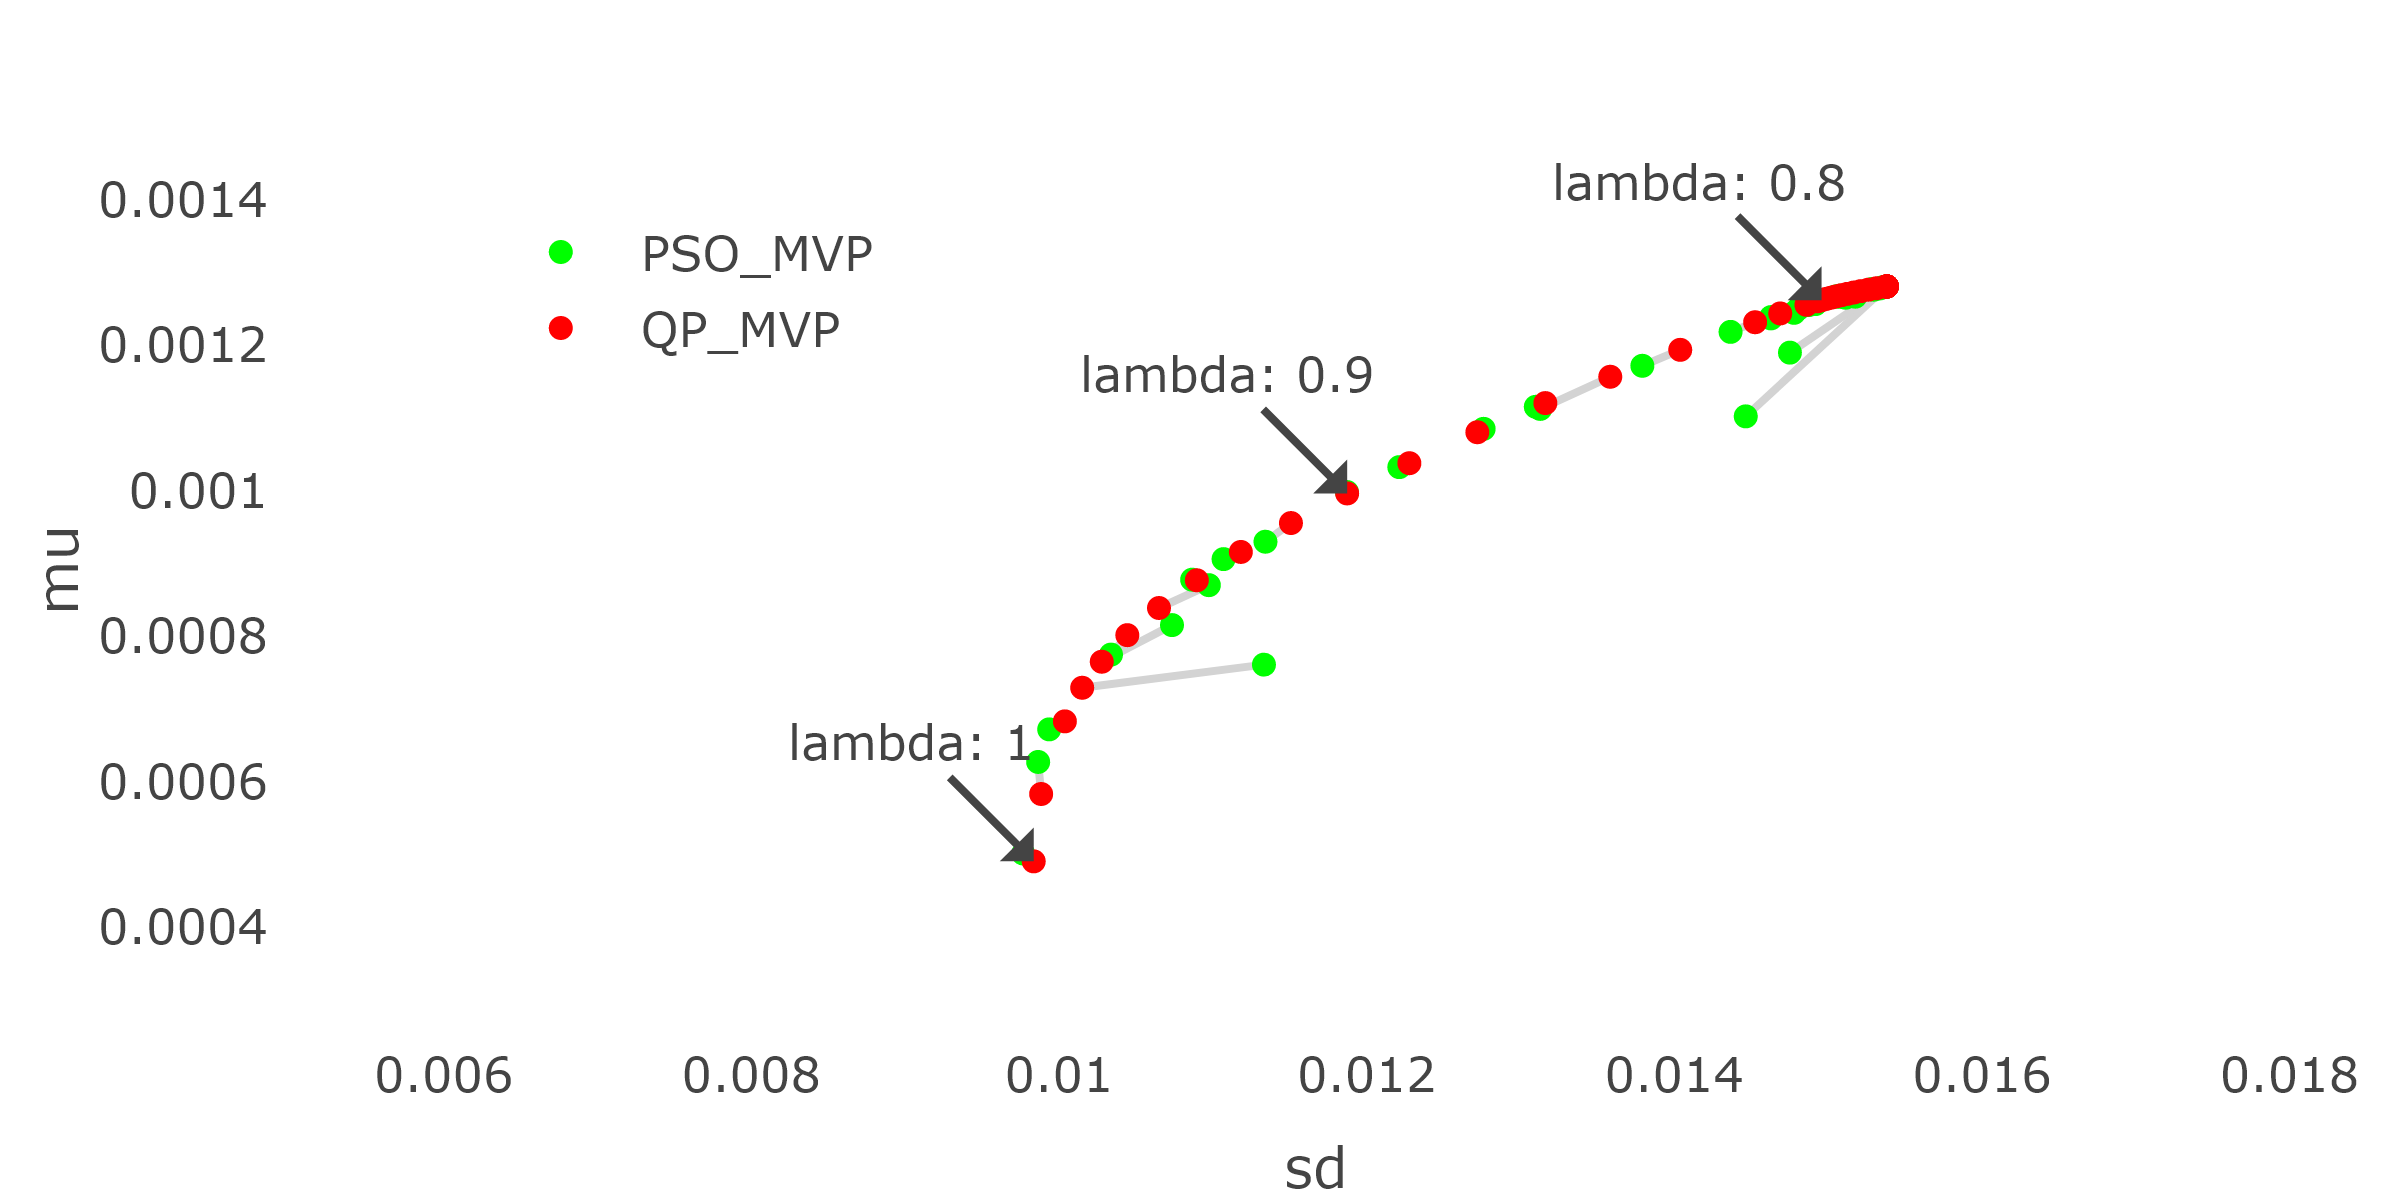
\includegraphics{Master_Thesis_files/figure-latex/pso7-1} \caption{Comparison of the MVP's generated with solve.QP and the PSO. The gray lines show the difference of the solutions of both approaches for each lambda}\label{fig:pso7}
\end{figure}

The corresponding portfolios for each \(\lambda\) are connected with a grey line to visualize the error of the PSO. It turns out that it is possible to solve MVP problems with a PSO approach. It is noticable that some PSO runs were not able to reach the global minimum and thus show a deviation from the \texttt{solve.QP} approach, which can often be fixed by repeated runs.

\hypertarget{example-itp-mste}{%
\section{Example ITP-MSTE}\label{example-itp-mste}}

A similar ITP-MSTE solved with \texttt{solve.QP} in section \ref{exampleitpsolveqp} is used as a benchmark for the PSO. In summary, the goal is to create a portfolio that minimizes the mean square error of the returns of itself and the SP500TR between 2018-01-01 and 2019-12-31. The pool of assets includes all assets that are present in 2019-12-31 and have no missing values. The constraints are long only and the weights should sum to one. The parameters for the PSO are a swarm size of 100, 100 iterations, the inertia weight starts at \(1.2\) and decreases to zero, the upper bound is \(0.05\), and a starting position is the equally weighted vector \(v\) with \(\textstyle\sum v_i=1\). The PSO was run ten times, and the aggregated best and mean runs are compared to the \texttt{solve.QP} approach for seed 0 in the table below:

\begin{figure}[H]
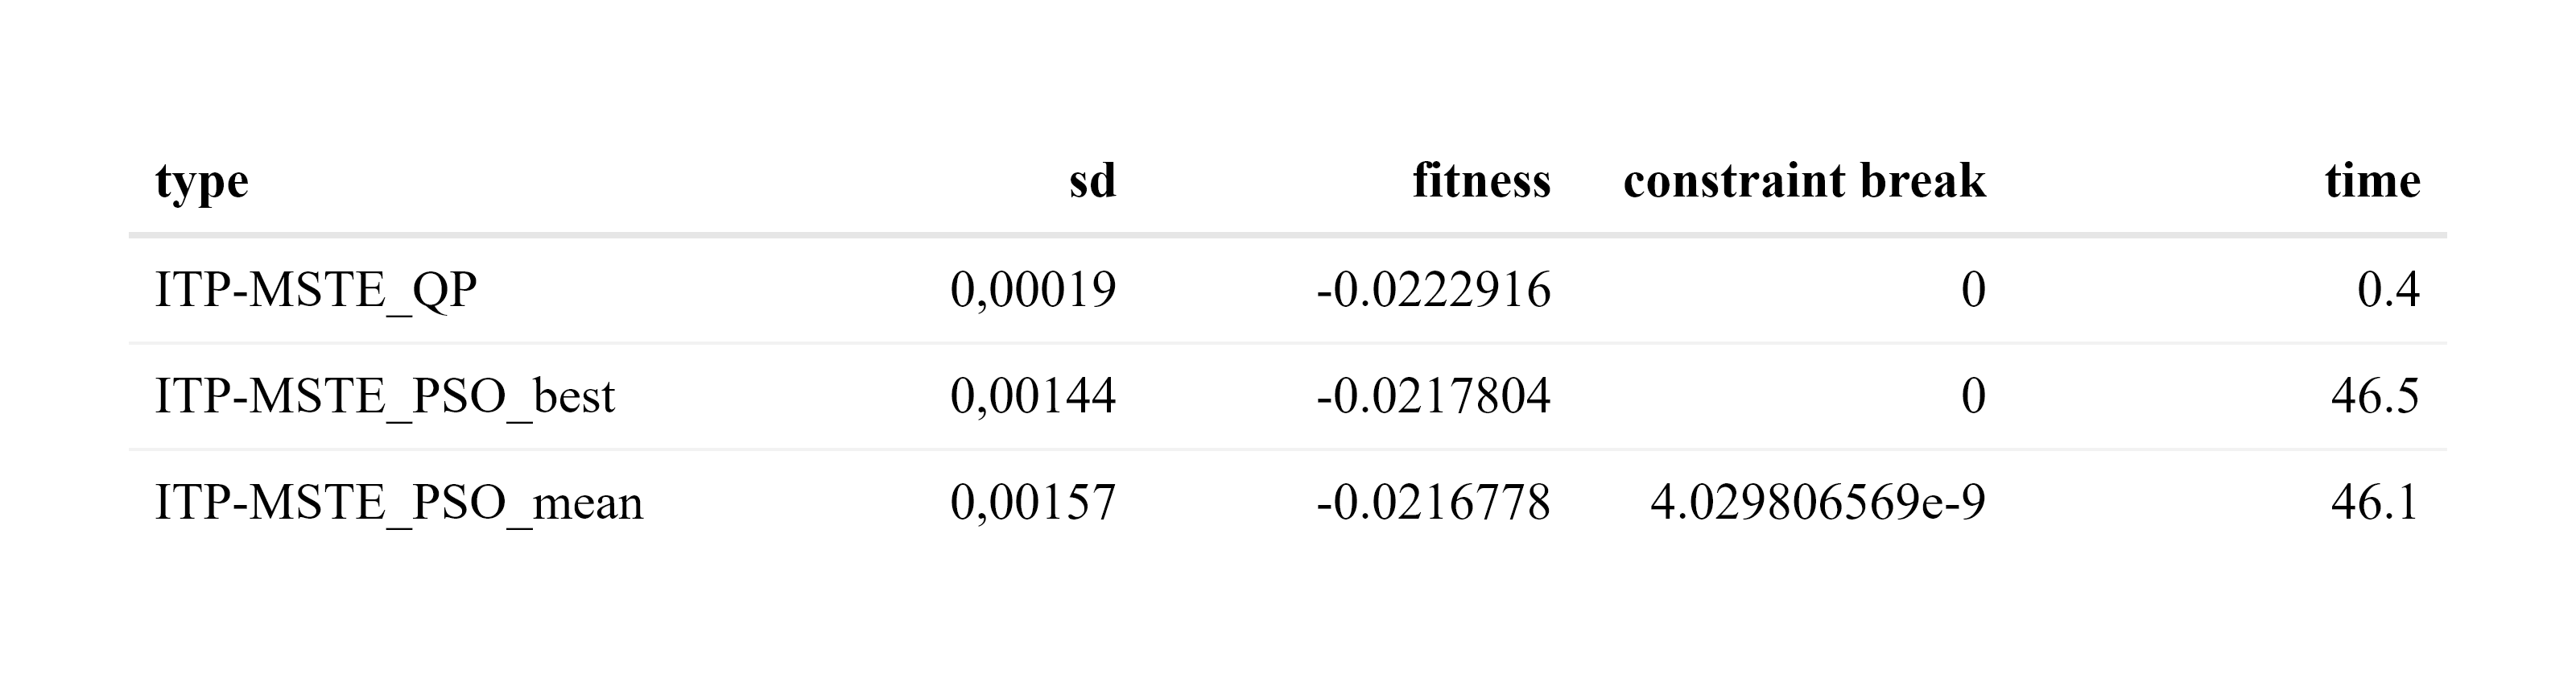
\includegraphics{Master_Thesis_files/figure-latex/pso8-1} \caption{Comparison of solving ITP-MSTE with solve.QP and the PSO}\label{fig:pso8}
\end{figure}

It can be seen that in all PSO runs, sufficient fitness was achieved with negligible constraint breaks, but much more computation time was required.

\hypertarget{pros-and-cons-for-continuous-problems}{%
\section{Pros and Cons for Continuous Problems}\label{pros-and-cons-for-continuous-problems}}

A PSO approach has advantages and disadvantages, since on the one hand any problem can theoretically be solved, but it cannot be guaranteed that the solution is also optimal. In addition, the calculations take much longer than with the \texttt{solve.QP} approach, which raises the question why a PSO approach should have any benefit at all. This is exactly the case, if the solution of the problem is no longer possible by the \texttt{solve.QP} alone, as it is for example the case with mixed-integer-quadratic-problems. In this type of problems, the condition is that the variable of interest \(x\) must be an integer vector, which can only be solved continuously using \texttt{solve.QP} and then rounded. However, this rounding error can become arbitrarily large, which is why the chances of the PSO approach to achieve a better solution are greater than with the \texttt{solve.QP} approach.

\hypertarget{discrete-problems}{%
\section{Discrete Problems}\label{discrete-problems}}

A continuous solution for a portfolio is not sufficient for practical purposes, since usually only integer amounts of assets can be purchased. It's even worse if lot sizes are needed, because these can only be bought in minimum denomination of e.g.~ten thousand. Lot sizes are often used in fixed income products. The biggest drawbacks of rounding a continuous solution are the disregarding of conditions and the difference in the objective value, which often can't reach the new optimum. A solution with broken conditions is not acceptable in practice and a \texttt{solve.QP} approach only produces one solution, which is why its insecure to hope for a sufficient solution after rounding. The PSO doesn't have these drawbacks and can be easily used for discrete problems by rounding the input of the objective function \texttt{fn()}. In a portfolio with net asset value (\texttt{nav}) consisting of only American stocks with weights \(w_i\) and closing prices \(p_i\) can be discretized to \(w_i^d\) by the following formula:

\[
  w_i^d =\text{round}(w_i \cdot \frac{\text{nav}}{p_i})\cdot \frac{p_i}{\text{nav}}.
\]

\hypertarget{example-discrete-itp-mste}{%
\section{Example Discrete ITP-MSTE}\label{example-discrete-itp-mste}}

This example analyses the error of rounding a solution with the \texttt{solve.QP} approach and compares it to a discrete PSO. A second discrete PSO is added, that takes the continuous solution of the \texttt{solve.QP} and uses it as starting position of one particle. The ITP-MSTE focuses on replicating the SP500TR with its top 100 assets derived from the example with discarding in section \ref{exampleitpsolveqp} and tries to construct a portfolio with the constraints long only, \(0.99 \leq \textstyle\sum w_i \leq 1\) and \(\text{nav} = 10000\) in the time frame from 2018-01-01 to 2019-12-31. The used prices are closing prices and both PSO's have 100 particles and 300 iterations. The results can be observed in the table below:

\begin{figure}[H]
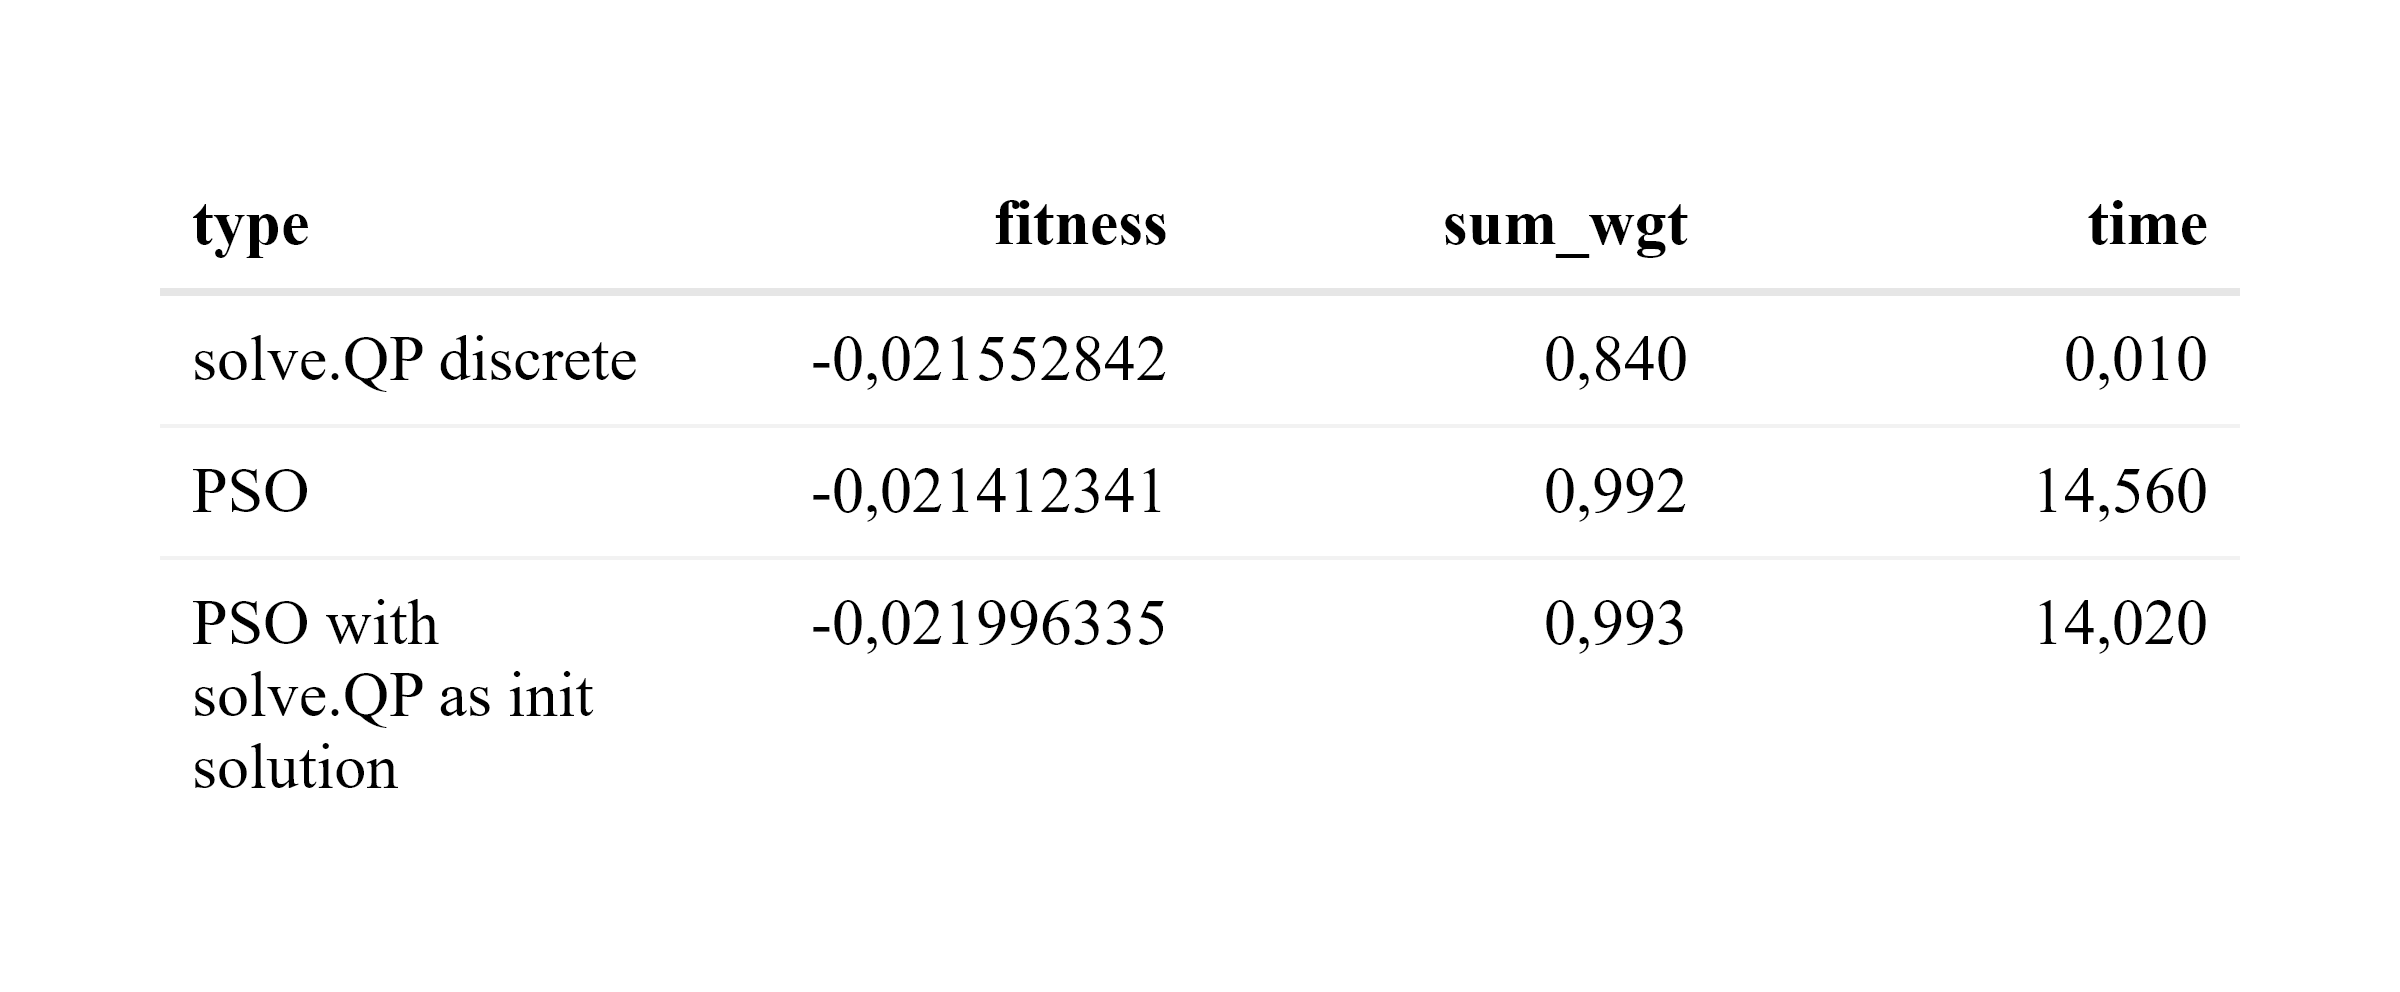
\includegraphics{Master_Thesis_files/figure-latex/pso9-1} \caption{Comparison of solving a discrete ITP-MSTE with PSO and the solve.QP with rounding afterwards}\label{fig:pso9}
\end{figure}

It can be seen that the rounded \texttt{solve.QP} solution still has a good fitness but the constraints are not satisfied. The PSO has no constraint breaks and better fitness than the rounded \texttt{solve.QP}. The PSO with \texttt{solve.QP} solution as starting position has beaten both approaches. This indicates that a hybrid approach consisting of both the \texttt{solve.QP} and afterwards the PSO for intelligent rounding with observed constraints would be a good heuristic for such problems in practice.

\hypertarget{psovariants}{%
\chapter{PSO Variations}\label{psovariants}}

The standard PSO analyzed in the previous chapter is capable of solving a wide range of problems, but often gets stuck in local minima. In this chapter, different variants of the standard PSO are analyzed using a problem from the financial domain. The first variant is the PSO with function stretching, which is designed to allow the PSO to escape from local minima if they are discovered. The second variant is the local PSO, which is designed to reduce the probability of getting stuck in local minima by limiting the spread of information in the swarm. The third variant, the PSO with feasibility preservation, tries to optimize within the feasibility space and therefore provide only feasible solutions. The last variant is the PSO with self-adaptive velocity, which tries to adjust the control parameters according to certain rules and randomness.

\hypertarget{testproblem-discrete-itp-mste}{%
\section{Testproblem Discrete ITP-MSTE}\label{testproblem-discrete-itp-mste}}

All variants are tested on a discrete ITP-MSTE to replicate the SP500TR with a tracking portfolio consisting of the top 50 assets in the S\&P 500 derived from the example with discarding in section \ref{exampleitpsolveqp}. The daily data used to solve the ITP ranges from 2018-01-01 to 2019-12-31, and the assets must be in the SP500TR at the end of the time frame and have no missing values. The tracking portfolio is discrete and has a net asset value of twenty thousand USD. The tracking portfolio is discretized using closing prices on 2019-12-31, and returns are calculated as simple returns using the adjusted closing prices. The maximum weighting for each asset is 10\% to reduce the dimension space of the problem. Additional constraints are long only and portfolio weights \(w\) should satisfy \(0.99 \leq \textstyle\sum w_i \leq 1\). All variants are run 100 times and compared to 100 runs of the standard PSO created in the previous chapter. The swarm size for the PSO and all variants is 50 and the iterations are set to 400. All PSO's start with the zero vector as the initial particle position to test the ability to find the feasible space.

The next plot analyzes the behavior of the 100 standard PSO runs in each iteration by plotting the median of the best fitness achieved in each iteration. The confidence bands for the 95\% and 5\% quantiles of the best fitness values are plotted in the same color as the median, with less transparency:

\begin{figure}[H]
\includegraphics{Master_Thesis_files/figure-latex/variants1s-1} \caption{Fitness of the standard PSO for comparison with later variants}\label{fig:variants1s}
\end{figure}

The aggregate statistics of the last iterations of all 100 runs can be found in the table below:

\begin{figure}[H]
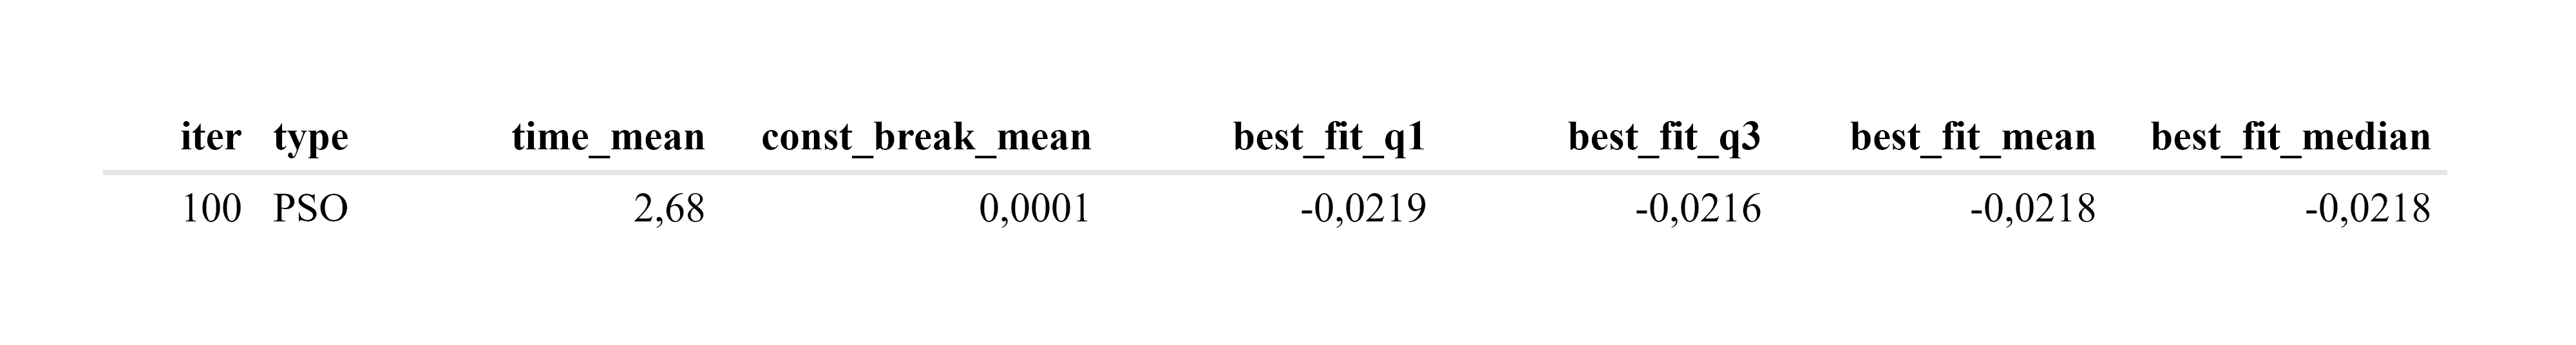
\includegraphics{Master_Thesis_files/figure-latex/variants2-1} \caption{Statistics of the standard PSO for comparison with later variants}\label{fig:variants2}
\end{figure}

\hypertarget{function-stretching}{%
\section{Function Stretching}\label{function-stretching}}

PSO often gets stuck in local minima, i.e.~when the current global best position is a local minimum with a surrounding region, with only higher fitnesses. In such situations, it is difficult for the PSO to escape to find the global minimum. Function stretching attempts to allow the PSO to escape such local minima by transforming the fitness function in the same way as described in \citep{PaVr2002}. After finding a local minimum, a two-stage transformation proposed by Vrahatis in 1996 can be used to stretch the original function such that the discovered local minimum is transformed into a maximum and any position with less fitness remains unchanged. The two stages of the transformation with a discovered local minimum \(\bar{x}\) are:

\begin{equation} 
G(x) = f(x) +  \gamma_1 \cdot \| x-\bar{x} \| \cdot (\text{sign}(f(x)-f(\bar{x}))+1)
\label{eq:fnstretchG}
\end{equation}
and
\begin{equation} 
  H(x) = G(x) + \gamma_2 \cdot \frac{\text{sign}\biggl(f(x)-f(\bar{x})\biggr)+1}{\text{tanh}\biggl( \mu \cdot (G(x)-G(\bar{x})) \biggr)}.
\label{eq:fnstretchH}
\end{equation}

The value \(G(\bar{x})\) can be simplified to \(f(\bar{x})\), the norm used in \(G(x)\) is the Manhattan norm and the \(\text{sign}()\) function is defined as follows:

\[
  \text{sign}(x) = 
  \begin{cases}
    1, & \text{if}\ \ x > 0\\
    0, & \text{if}\ \ x = 0\\
    -1, & \text{if}\ \ x < 0.
  \end{cases}
\]

In the source it is suggested to select the following parameter values as default:

\begin{align*}
  \gamma_1 &= 5000 \\
  \gamma_2 &= 0.5 \\
  \mu &= 10^{-10}.
\end{align*}

It is difficult to interpret both transformations accurately, especially in higher dimensions, but some concepts can be recognized by looking only at the most important parts. The first transformation \(G(x)\) uplifts all values greater than or equal to the local minimum and increases the uplift as a function of distance from the local minimum. The second function \(H(x)\) also does not change any values below the local minimum and otherwise focuses on all values near the local minimum, stretching it to infinity and dropping steeply to repel particles.

To better understand the transformation, it is used to stretch a simple function in \(\mathbb{R}^1\) defined as follows:

\[
f(x) = cos(x)+\frac{1}{10}\cdot x
\]

and translated to the objective function:

\vspace{0.1cm}\fontsize{11}{12}\selectfont

\begin{Shaded}
\begin{Highlighting}[]
\NormalTok{fn }\OtherTok{\textless{}{-}} \ControlFlowTok{function}\NormalTok{(pos)\{}
  \FunctionTok{cos}\NormalTok{(pos) }\SpecialCharTok{+} \DecValTok{1}\SpecialCharTok{/}\DecValTok{10} \SpecialCharTok{*}\NormalTok{ pos}
\NormalTok{\}}
\end{Highlighting}
\end{Shaded}

\normalsize\vspace{0.1cm}

The domain of definition is chosen as \(x \in [-20, 20]\). Suppose the PSO gets stuck in the local minimum at \(\bar{x} = \pi - \text{arcsin}(\frac{1}{10}) \approx 3.04\). The original function \texttt{fn} and the transformed function \texttt{fn\_stretched}, which matches \(H(x)\) in equation \eqref{eq:fnstretchH}, are shown in the following graph:

\begin{figure}[H]
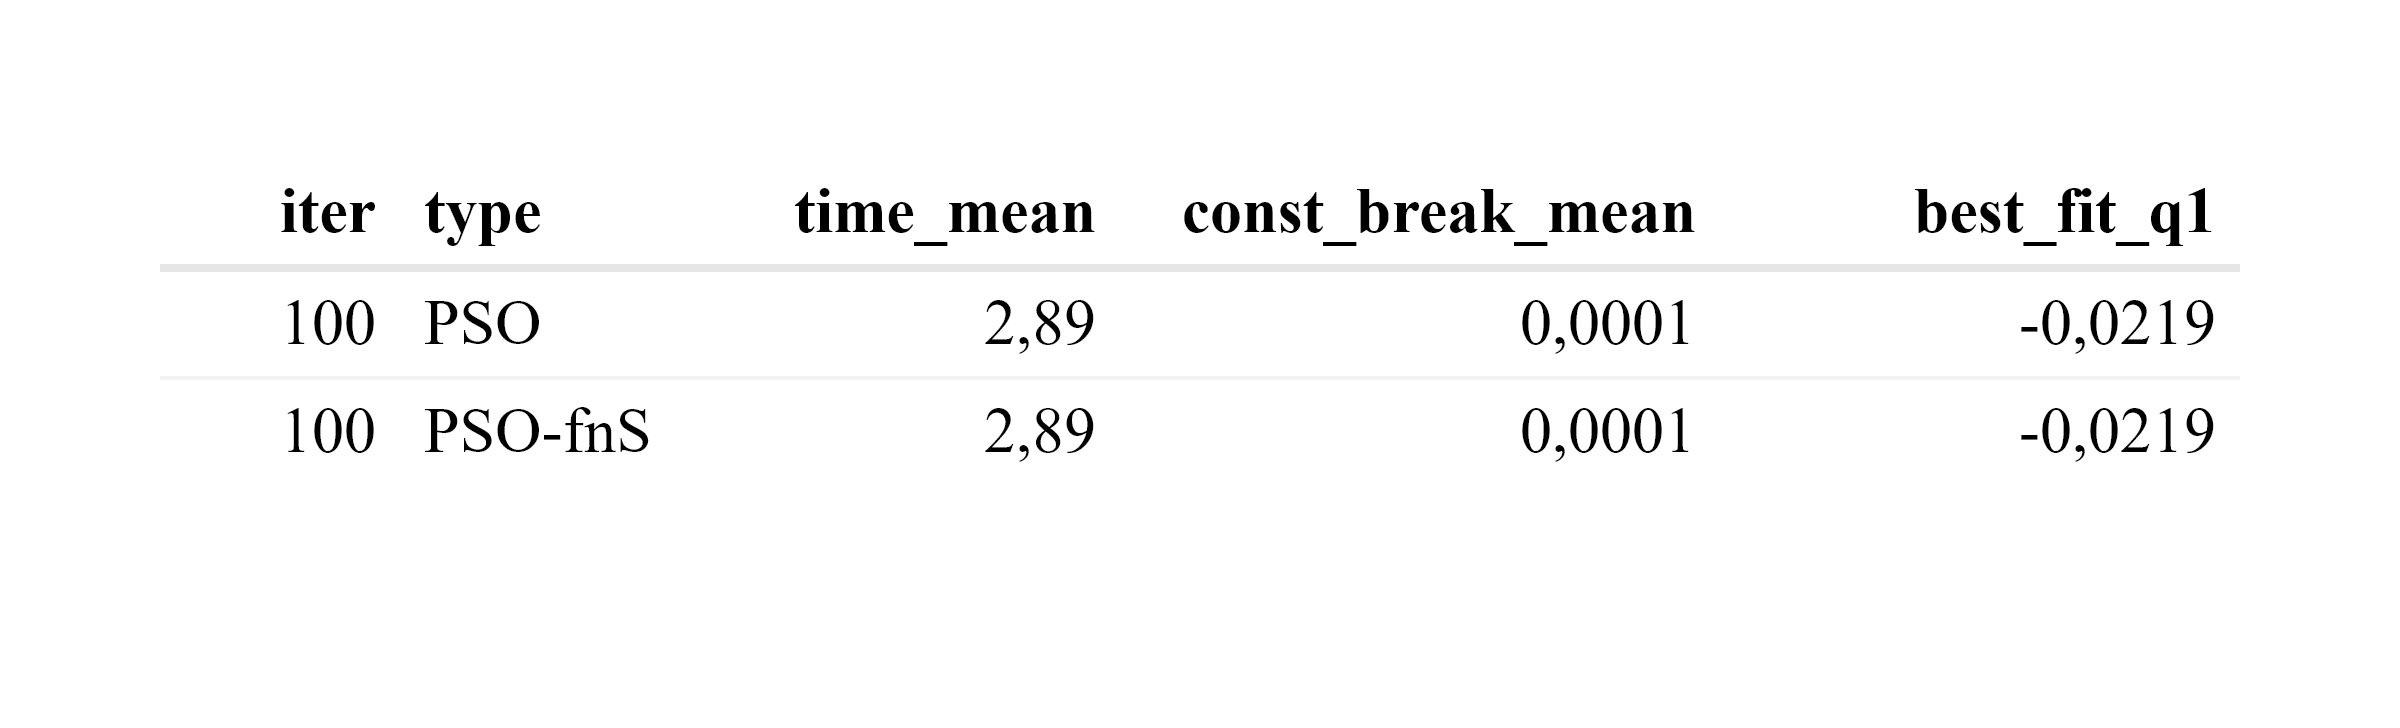
\includegraphics{Master_Thesis_files/figure-latex/unnamed-chunk-11-1} \caption{The effect of function stretching in a 1D example}\label{fig:unnamed-chunk-11}
\end{figure}

It can be seen that the fitness is stretched upward around the local minimum \(\bar{x}\), making it much easier for the PSO to go down the hill and fall into new minima with lower fitness. It can be observed that on the right hand side there was only higher fitness before and after the transformation a local minimum has emerged which has a large area where only higher fitness values are located. In the worst case this can lead to a new local minimum from which it is even more difficult to escape. All regions with lower fitness remain unchanged, as can be seen in the zoomed version of the bottom diagram from above:

\begin{figure}[H]
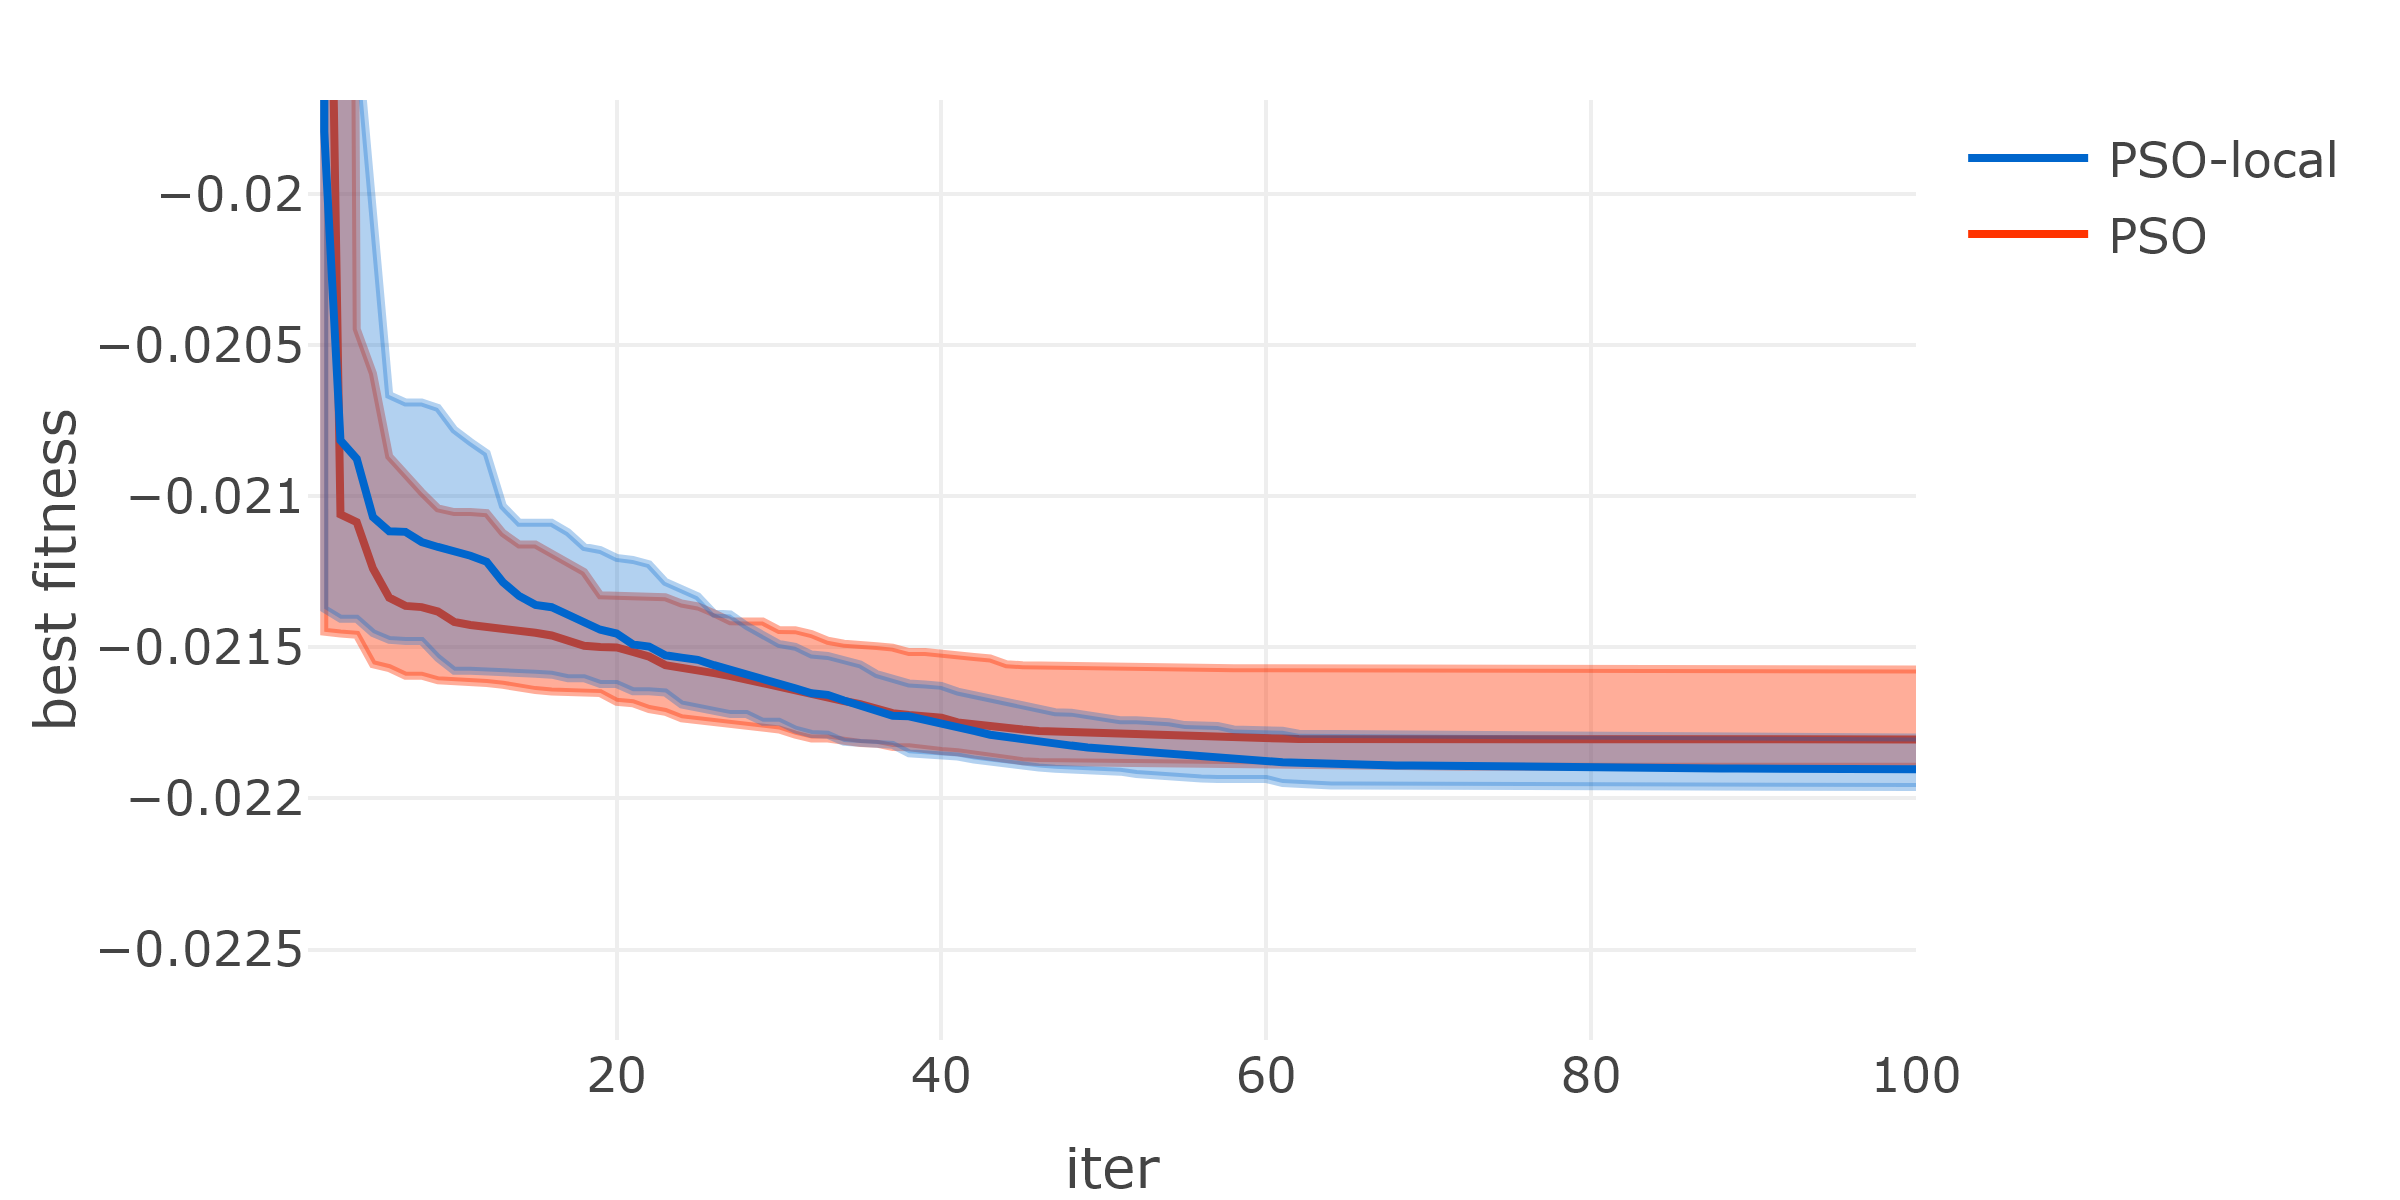
\includegraphics{Master_Thesis_files/figure-latex/unnamed-chunk-12-1} \caption{Zoomed version of the lower graphic from the figure above}\label{fig:unnamed-chunk-12}
\end{figure}

\hypertarget{implementation}{%
\subsection{Implementation}\label{implementation}}

Since it is not possible to know if the PSO is stuck in a local minimum, a stagnation value was added that increases by one if the global best particle does not change. After ten iterations with no change, a local minimum is assumed and the transformation of the original objective function \(f(x)\) takes place. After that, all personal best fitness values must be re-evaluated to work with the evaluated space and the stagnation value is set to zero. To prevent transformation just at the end of all iterations, the current iteration must be less than the maximum iteration minus twenty to allow transformation to occur. The transformed function \(H(x)\) remains the objective function until the next local minimum is suspected, which again leads to a transformation of the original function \(f(x)\).

\hypertarget{test-pso-with-function-stretching}{%
\subsection{Test PSO with Function Stretching}\label{test-pso-with-function-stretching}}

The PSO with function stretching is called \texttt{PSO-fnS} and is evaluated on the test problem with \(\gamma_1 = 5000\), \(\gamma_2 = 0.5\) and \(\mu = 10^{-10}\):

\begin{figure}[H]
\includegraphics{Master_Thesis_files/figure-latex/variants3s-1} \caption{Comparison of fitness between the PSO with functional stretching and the standard PSO}\label{fig:variants3s}
\end{figure}

The aggregate statistics of the last iterations of all 100 runs can be found in the table below:

\begin{figure}[H]
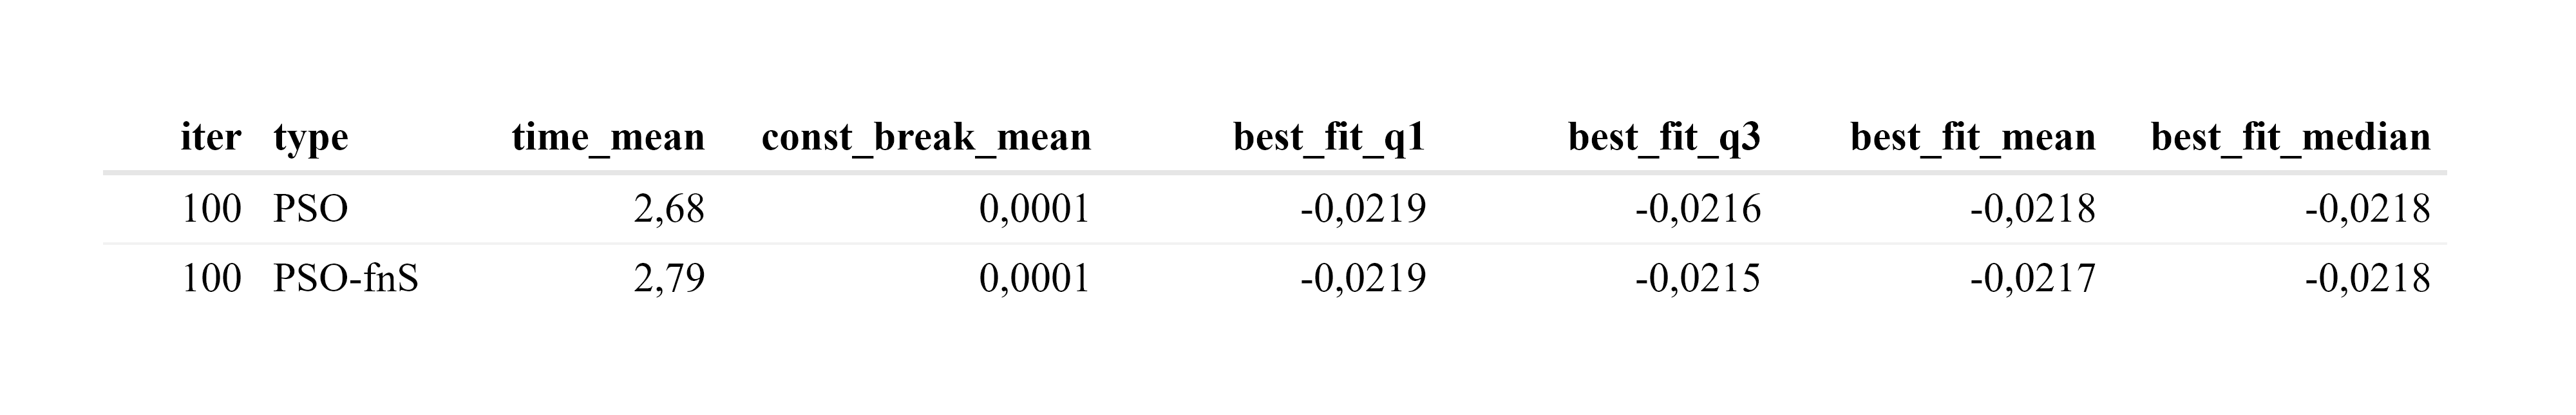
\includegraphics{Master_Thesis_files/figure-latex/variants4-1} \caption{Comparison of statistics between the PSO with functional stretching and the standard PSO}\label{fig:variants4}
\end{figure}

It turns out that functional stretching does not provide any benefits in this particular problem. Perhaps it is due to the unfavorable values for \(\gamma_1\), \(\gamma_2\) and \(\mu\), which lead to too strong repulsion of the particles. Another reason could be that the stretching of the function generates new local minima which are even more difficult to overcome than the original ones, especially in higher dimensions.

\hypertarget{local-pso}{%
\section{Local PSO}\label{local-pso}}

The local PSO is a more general case of the standard PSO, which is also referred to as global PSO. The only difference is the selection of the global best particle by defining a neighborhood. Each particle \(x_i\) has a neighborhood \(N(x_i, \bar{k})\), and the global best particle in its neighborhood is called the local best particle of \(x_i\). If the neighborhood is chosen large enough to contain all particles, it corresponds to the standard PSO (global PSO). A simple definition of a neighborhood with \(k\) neighbors for particles \(x_i\) given in \citep{Enge2013} would be:

\[
  N(x_i, k) = \{ x_{i-\bar{k}}, x_{i-(\bar{k}-1)}, x_{i-(\bar{k}-2)}, \cdots, x_{i}, \cdots, x_{i+(\bar{k}-2)}, x_{i+(\bar{k}-1)}, x_{i+\bar{k}} \}
\]

with

\[
  \bar{k} = floor(\frac{k}{2}) = \lfloor \frac{k}{2} \rfloor.
\]

To illustrate this, the following figure defines the neighborhoods \(N(x_3, 4)\) and \(N(x_1, 4)\):

\begin{figure}
\centering
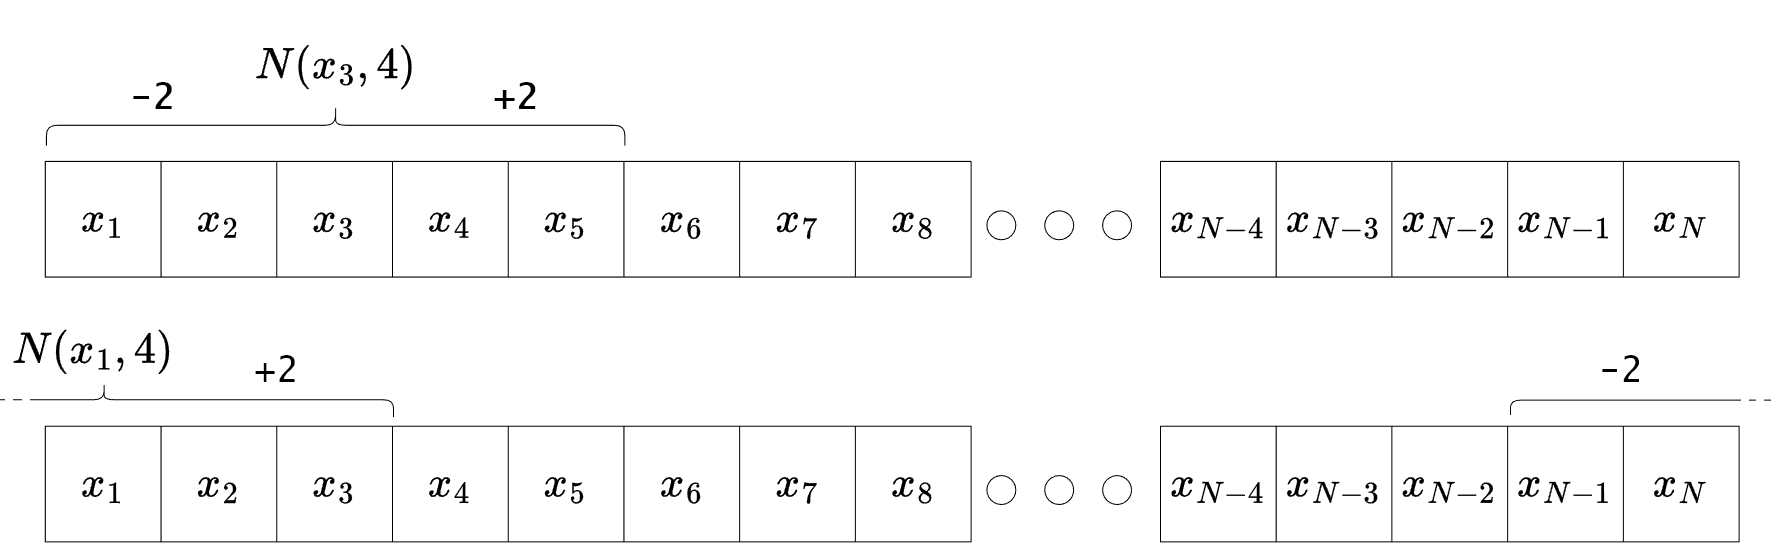
\includegraphics{img/PSO_local_chart4444.png}
\caption{Visualization of the simple neighborhood topology.}
\end{figure}

In the latter case, it can be seen that the overflowing boundary will continue on the opposite side of the arranged particles.

\hypertarget{implementation-1}{%
\subsection{Implementation}\label{implementation-1}}

First, the neighbors for each particle are stored in a suitable data structure before the main part of the PSO is executed. In the local version there is no global best particle, instead the global best particle for the neighborhood of each particle has to be calculated in each step.

\hypertarget{test-local-pso}{%
\subsection{Test Local PSO}\label{test-local-pso}}

The PSO with particle neighborhoods is called \texttt{PSO-local} and is evaluated on the test problem with \(k=10\):

\begin{figure}[H]
\includegraphics{Master_Thesis_files/figure-latex/variants5s-1} \caption{Comparison of fitness between the local PSO and the standard PSO}\label{fig:variants5s}
\end{figure}

The aggregate statistics of the last iterations of all 100 runs can be found in the table below:

\begin{figure}[H]
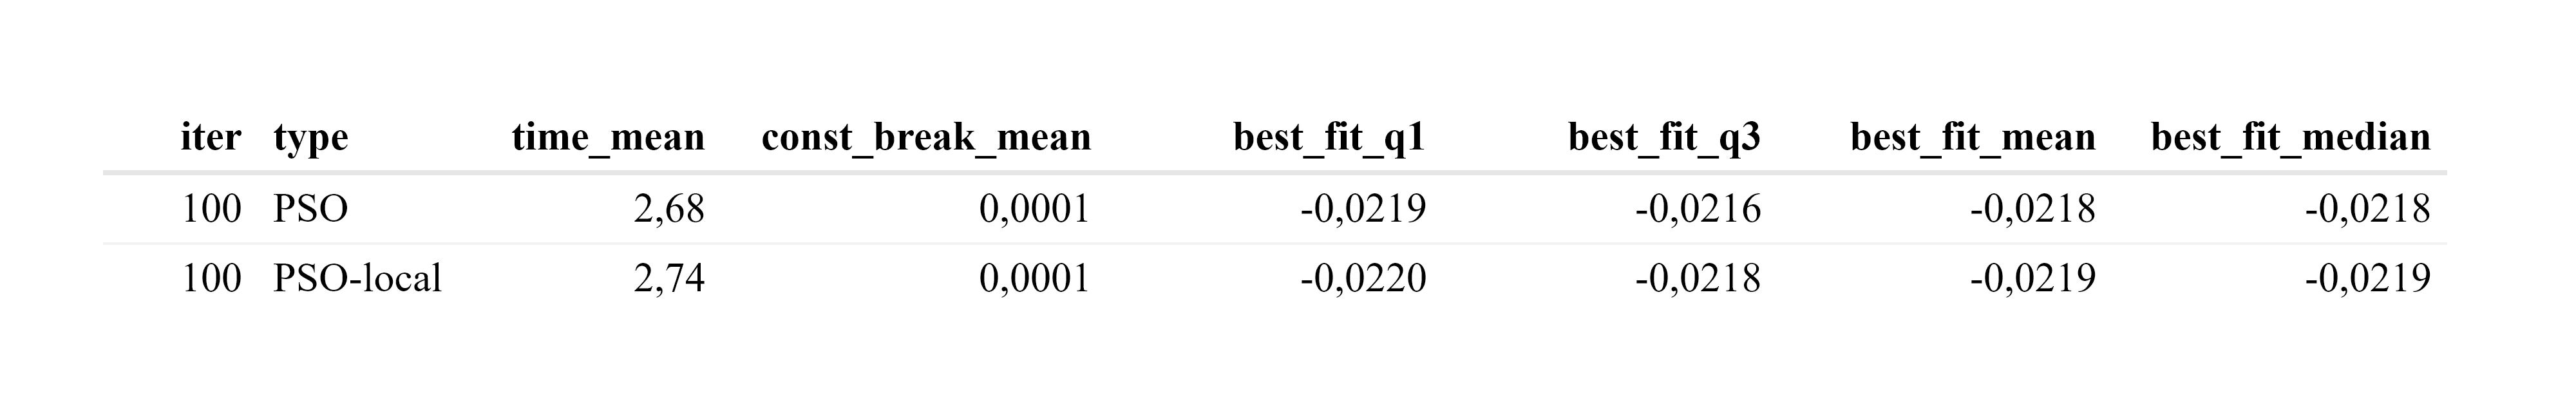
\includegraphics{Master_Thesis_files/figure-latex/variants6-1} \caption{Comparison of statistics between the local PSO and the standard PSO}\label{fig:variants6}
\end{figure}

It can be seen that it is superior to the standard PSO in this case. Especially in preventing stagnation in local minimas, which can be seen in the narrower quantile bands at the end.

\hypertarget{preserving-feasibility}{%
\section{Preserving Feasibility}\label{preserving-feasibility}}

Other variants of PSO often provide solutions that are infeasible, resulting in the need to run them multiple times. To ensure that each solution is feasible, a new variant was created in \citep{XiEb2002} that preserves the feasibility of the solutions. To be precise, this is not a variant of its own, but rather a different method for handling constraints instead of the commonly used penalty method. Nevertheless, it must change the core of the PSO implementation, which is why it is classified as its own variant in this work. The difference to the standard PSO is that the initialization of the particles is repeated until all positions are feasible. After that, only feasible solutions are stored as global or personal best positions, resulting in a guaranteed feasible final solution. Even the first step is the most difficult to achieve in practice. To illustrate this, the result of trying to find a feasible position among a million randomly generated positions of the test problem looks like this:

\begin{verbatim}
[1] "Feasable positions: 0"
\end{verbatim}

\begin{verbatim}
[1] "Elapsed time: 153.4 seconds"
\end{verbatim}

It can be seen that after a million randomly generated positions, there was not a single feasible position. For this reason, the first step has been modified to start with only one feasible position, randomly selected from one of the final solutions of the standard PSO. The standard PSO was also repeated with the same starting positions to allow comparison.

\hypertarget{test-preserving-feasibility-pso}{%
\subsection{Test Preserving Feasibility PSO}\label{test-preserving-feasibility-pso}}

This section compares the PSO with feasibility preservation and the standard PSO. Both PSOs use the same feasible solutions as starting positions:

\begin{figure}[H]
\includegraphics{Master_Thesis_files/figure-latex/variants6nextss-1} \caption{Comparison of fitness between the PSO with feasibility preservation and the standard PSO, starting from the same randomly selected initial particles obtained from the last iterations of the standard PSO solutions}\label{fig:variants6nextss}
\end{figure}

The aggregate statistics of the last iterations of all 100 runs can be found in the table below:

\begin{figure}[H]
\includegraphics{Master_Thesis_files/figure-latex/variants6next2-1} \caption{Comparison of statistics between the PSO with feasibility preservation and the standard PSO, starting from the same randomly selected initial particles obtained from the last iterations of the standard PSO solutions}\label{fig:variants6next2}
\end{figure}

The results indicate that the PSO with feasibility preservation is not able to solve finance-related problems that have a very small feasible space. It is more efficient to repeat the PSO with the previous best position until the solution is feasible.

\hypertarget{self-adaptive-velocity}{%
\section{Self-Adaptive Velocity}\label{self-adaptive-velocity}}

A PSO approach with self-adaptive velocity that attempts to reduce hyperparameters was analyzed in \citep{FaYa2014}. The self-adaptive velocity is enabled by multiple velocity update schemes that are used randomly. Moreover, all hyperparameters are self-adaptive, since each particle has its own coefficients \(c_g\), \(c_p\), and \(w\), which change after each iteration depending on the fitness and other factors. The resulting PSO has no real hyperparameters that need to be tuned, and thus can be used as a general-purpose PSO.

\hypertarget{implementation-2}{%
\subsection{Implementation}\label{implementation-2}}

The process of this PSO variant is significantly different from the standard PSO, so all changes are summarized in steps.

1) Initialize: Each particle \(d\) must initialize its own inertial weight \(w_d^0=0.5\) and acceleration coefficients \(c_{p,d}^0 = c_{g,d}^0 = 2\).

2) Velocity and positions: Update the velocity of each particle \(d\) with the following switch-case for a uniform random number \(r = \text{Unif}(0,1)\) in iteration \(i+1\):

\begin{align*}
  v_d^{i+1} &= w_d^i \cdot v_d^{i}+c_{p,d}^i \cdot Z \cdot (p_{p,d}^i-x_d^i) + c_{g,d}^i \cdot Z \cdot (p_{g}^i-x_d^i) \\
  Z &= \begin{cases}
    \text{Unif}(0,1), & \text{if}\ \ r > 0.8\\
    \text{Cauchy}(\mu_1, \sigma_1), & \text{if}\ \ 0.8 \geq r > 0.4\\
    \text{Cauchy}(\mu_2, \sigma_2), & \text{if}\ \ 0.4 \geq r\\
  \end{cases}
\end{align*}

with

\begingroup
\allowdisplaybreaks

\begin{align*}
  \mu_1 &= 0.1 \cdot (1-(\frac{i}{i_{max}})^2) + 0.3 \\
  \sigma_1 &= 0.1 \\
  \mu_2 &= 0.4 \cdot (1-(\frac{i}{i_{max}})^2) + 0.2 \\
  \sigma_2 &= 0.4
\end{align*}
\endgroup

and \(\text{Cauchy}(\mu, \sigma)\) is a random number generated from the Cauchy distribution obtained with \texttt{rcauchy()} in R. The position update is the same as for the standard PSO. When a particle \(d\) has left the feasible search space in its coordinate \(z\), it is moved back with the following switch-case for \(r = \text{Unif}(0,1)\):

\[
  x_{z,d} = 
  \begin{cases}
    \text{generate uniform in the defined space}, & \text{if}\ \ r > 0.7\\
    \text{push back to boundary}, & \text{otherwise.}\ \ \\
  \end{cases}
\]

3) Fitness evaluation: In the same way as for the standard PSO.

4) Self-adaptive control parameters: For an objective function \(f()\) and the maximum fitness of all particles \(f_{max} = \text{max}(f(X^{i+1}))\), the parameters \(w_d^{i}\), \(c_{p,d}^{i}\) and \(c_{g,d}^{i}\) are adjusted for each particle \(d\) as follows:

\begin{align*}
  W^i_d &= \frac{\left| f(x_d^{i+1})-f_{max} \right|}{\sum_d\left| f(x_d^{i+1})-f_{max} \right|} \\
  w_d^{i+1} &= \text{Cauchy}(\sum_d W^i_d \cdot w_d^{i}, 0.2) \\
  c_{p,d}^{i+1} &= \text{Cauchy}(\sum_d W^i_d \cdot c_{p,d}^{i}, 0.3) \\
  c_{g,d}^{i+1} &= \text{Cauchy}(\sum_d W^i_d \cdot c_{g,d}^{i}, 0.3).
\end{align*}

Then, the parameters are adjusted to their limits using the following formulas:

\begin{align*}
w_d^{i+1} &= 
  \begin{cases}
    \text{Unif}(0,1), & \text{if}\ \ w_d^{i+1} > 1\\
    \text{Unif}(0,0.1), & \text{if}\ \  w_d^{i+1} < 0\\
    w_d^{i+1}, & \text{otherwise}
  \end{cases}\\
c_{p,d}^{i+1} &= 
  \begin{cases}
    \text{Unif}(0,1) \cdot 4, & \text{if}\ \ c_{p,d}^{i+1} > 4\\
    \text{Unif}(0,1), & \text{if}\ \  c_{p,d}^{i+1} < 0\\
    c_{p,d}^{i+1}, & \text{otherwise}
  \end{cases}\\
c_{g,d}^{i+1} &= 
  \begin{cases}
    \text{Unif}(0,1) \cdot 4, & \text{if}\ \ c_{g,d}^{i+1} > 4\\
    \text{Unif}(0,1), & \text{if}\ \  c_{g,d}^{i+1} < 0\\
    c_{g,d}^{i+1}, & \text{otherwise.}
  \end{cases}\\
\end{align*}

5) Update the best positions: Update the personal best \(P\) and global best \(p_g\) positions as in the standard PSO.

6) Repeat: Steps 2 to 5 are repeated until the maximum iteration \(i_{max}\) is reached.

\hypertarget{analyse-implementation}{%
\subsection{Analyse Implementation}\label{analyse-implementation}}

The random use of the distributions for the velocity update increases the diversity of the swarm. The coefficients in iteration \(i\) with 100 maximum iterations are distributed as follows:

\begin{figure}[H]
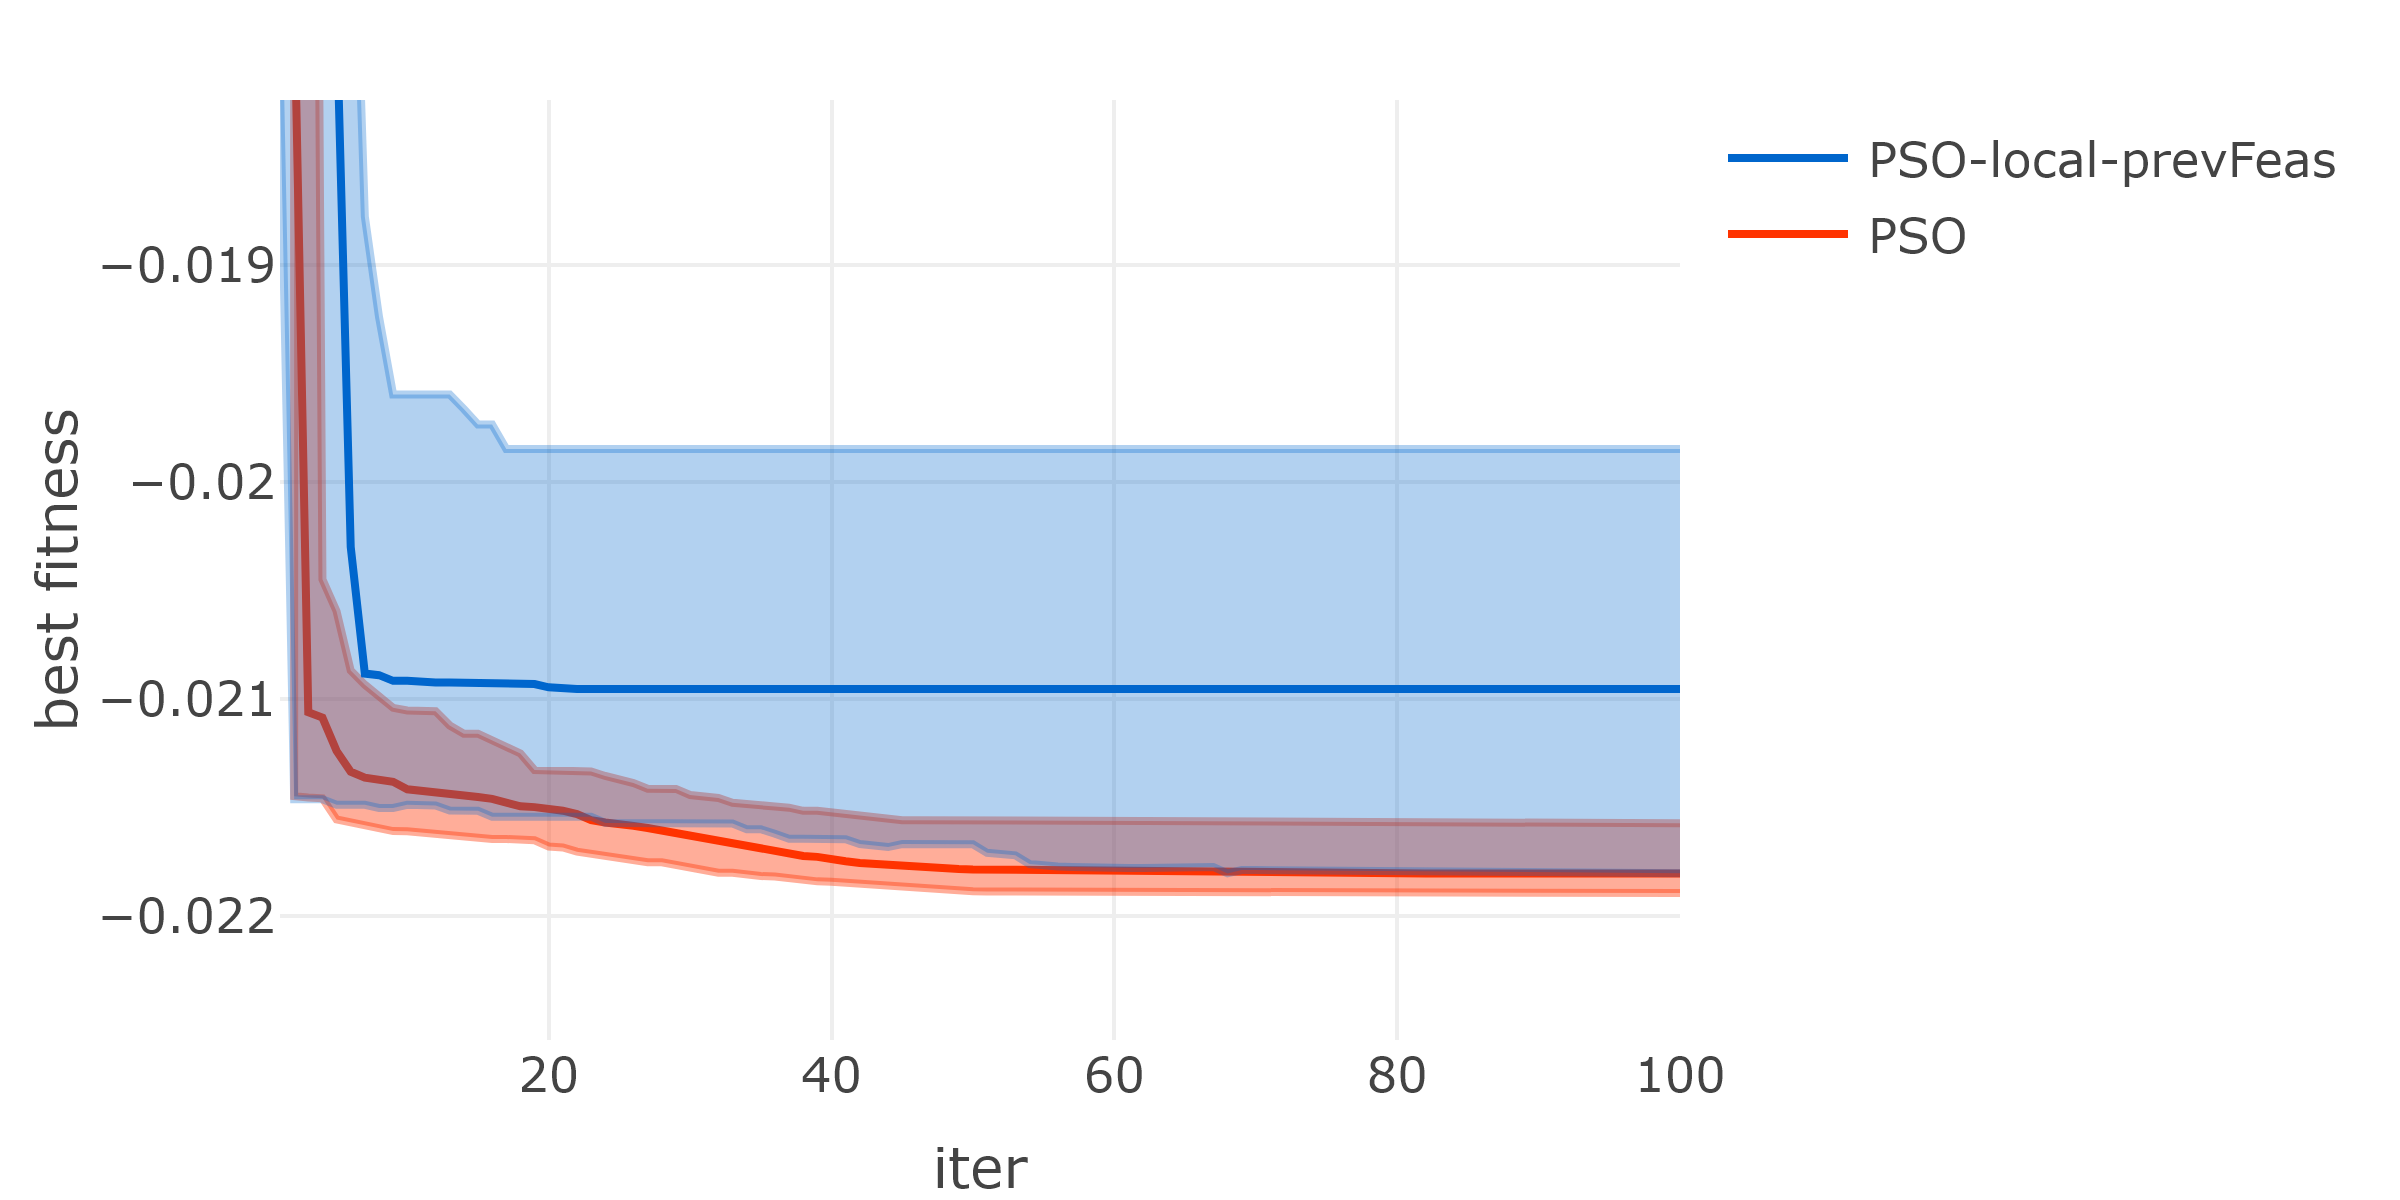
\includegraphics{Master_Thesis_files/figure-latex/unnamed-chunk-14-1} \caption{Comparison of the different distributions used in the velocity update of the PSO with self-adapting velocity depending on the iteration}\label{fig:unnamed-chunk-14}
\end{figure}

It can be seen that the randomness of the motion increases compared to the uniform distribution and the center of the Cauchy distributions slowly decreases towards the absolute term. In addition, the two Cauchy distributions differ in explorability and exploitability, indicated by probabilities outside \([0, 1]\).

Even more difficult to interpret is the adjusting of the control parameters. The value \(W_d^i\) is a weighting of the distances to the worst fitness, resulting in a higher weighting of the particles with good fitness. Later, the control parameters are adjusted using the Cauchy distribution with a weighted value of the previous control parameters as the center, giving higher weights to the control parameters that produced better fitness. This results in random control parameters distributed around the best previous control parameters. The resulting behavior can be described with a small quote, ``If exploration is beneficial, more exploration is done. If not, more is exploited.''

\hypertarget{test-pso-with-self-adaptive-velocity}{%
\subsection{Test PSO with Self-Adaptive Velocity}\label{test-pso-with-self-adaptive-velocity}}

The PSO with self-adaptive velocity is called \texttt{PSO-SAvel} and is evaluated for the test problem with the constants used in the implementation section:

\begin{figure}[H]
\includegraphics{Master_Thesis_files/figure-latex/variants7s-1} \caption{Comparison of fitness between the PSO with self-adaptive velocity and the standard PSO}\label{fig:variants7s}
\end{figure}

The aggregate statistics of the last iterations of all 100 runs can be found in the table below:

\begin{figure}[H]
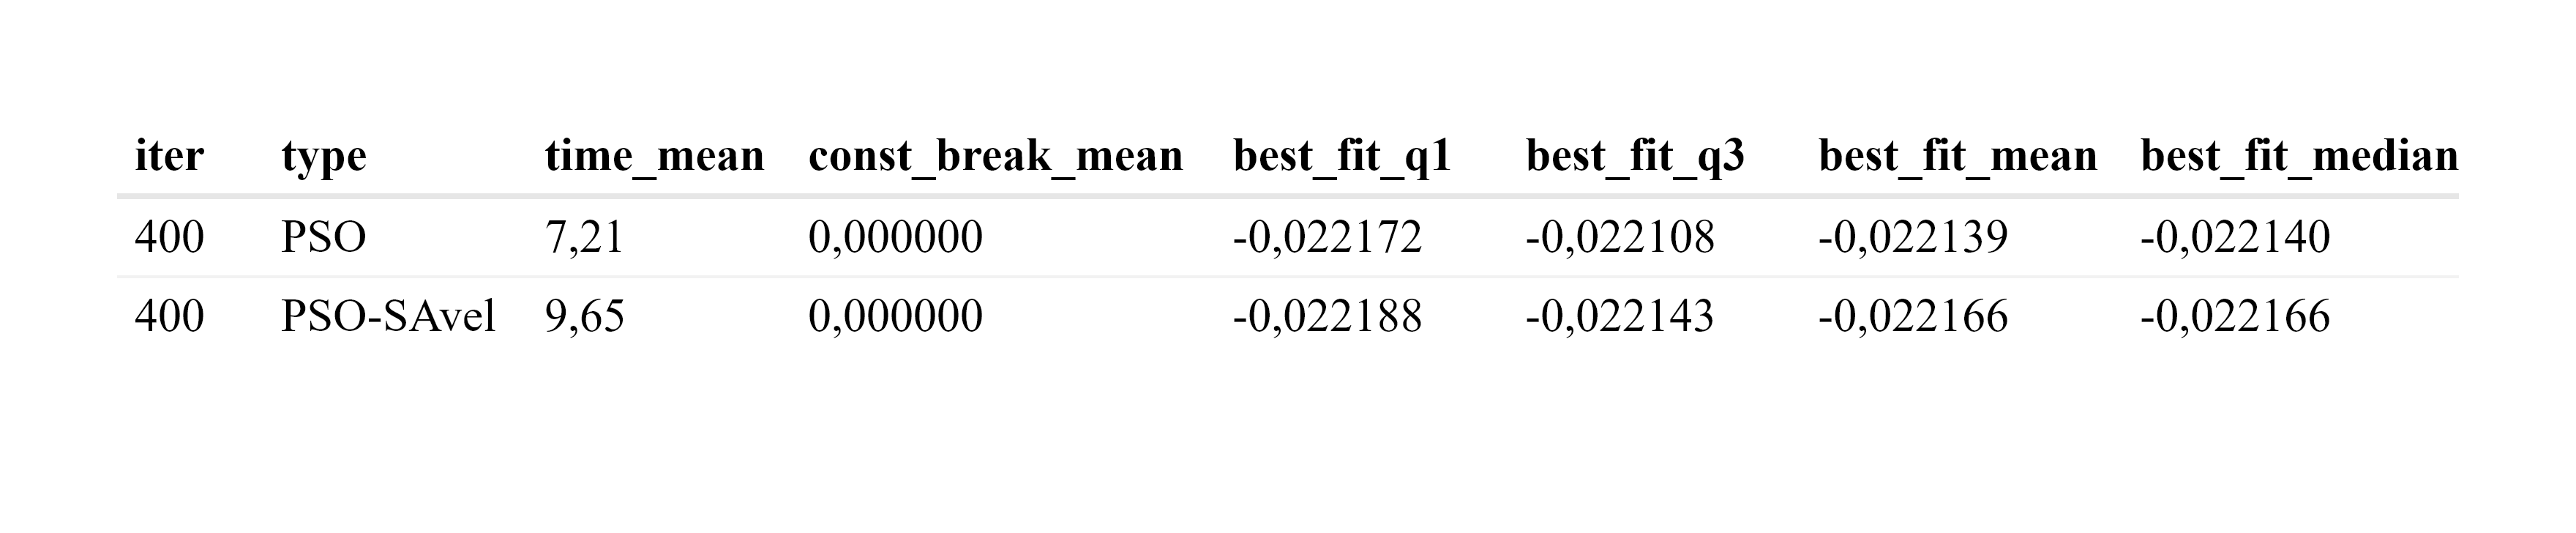
\includegraphics{Master_Thesis_files/figure-latex/variants8-1} \caption{Comparison of statistics between the PSO with self-adaptive velocity and the standard PSO}\label{fig:variants8}
\end{figure}

\vspace{-0.1cm}

The results look very promising, and with fewer hyperparameters to fine-tune, this may be one of the best variants for general use of a PSO.

\hypertarget{pso-r-package}{%
\section{PSO R Package}\label{pso-r-package}}

In this section, the existing package \texttt{pso} is used to compare the results with the standard PSO. The PSO from the existing package is called \texttt{PSO-pkg} and has been reconfigured to have the same hyperparameters as the standard PSO. It must be said that the \texttt{PSO-pkg} differs in the initialization of the velocity and does not use the compression coefficient of one tenth of the initialized velocity. The diagram below compares the fitness:

\vspace{-0.1cm}

\begin{figure}[H]
\includegraphics{Master_Thesis_files/figure-latex/variantspkgs-1} \caption{Comparison of fitness between the PSO R package with standard PSO settings and the standard PSO}\label{fig:variantspkgs}
\end{figure}

\vspace{-0.1cm}

The aggregate statistics of the last iterations of all 100 runs can be found in the table below:
\vspace{-0.2cm}

\begin{figure}[H]
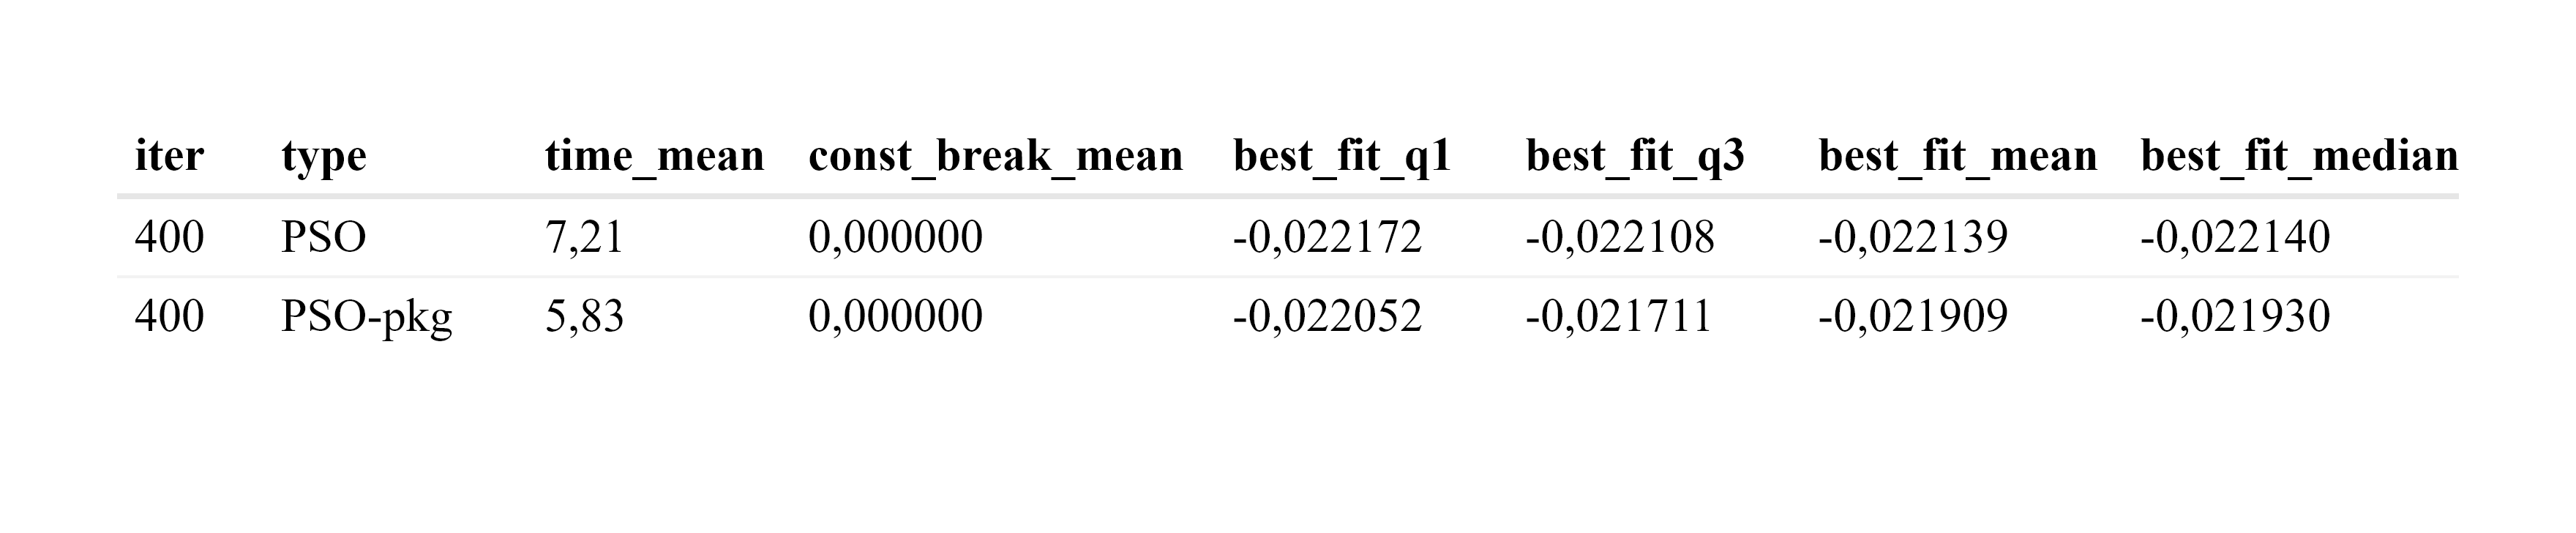
\includegraphics{Master_Thesis_files/figure-latex/variants9-1} \caption{Comparison of statistics between the PSO R package with standard PSO settings and the standard PSO}\label{fig:variants9}
\end{figure}
\vspace{-0.5cm}

The \texttt{PSO-pkg} is slightly different from the standard PSO, which is most likely due to the different velocity initialization. It is important to note that the package \texttt{pso} has many features and variants that are disabled for this comparison.

\hypertarget{comparison-with-other-metaheuristics}{%
\section{Comparison with other Metaheuristics}\label{comparison-with-other-metaheuristics}}

In addition to the PSO, there are other metaheuristics that also treat the optimization problem as a black box and can thus be brought to a generic form. This is exactly what has been done in the R package \texttt{metaheuristicOpt} by implementing 19 more metaheuristics besides the PSO. Therefore, this package can be used to compare which metaheuristic is suitable for a specific type of optimization problem. The implemented metaheuristics are the standard versions, which is why no statement about variants of these metaheuristics can be given. Likewise, it is not guaranteed how performant the respective metaheuristics have been implemented. Nevertheless, this package is a great help to quickly and easily test different metaheuristics for an explicit problem. The metaheuristics implemented in the R package \texttt{metaheuristicOpt} are the following:

\begin{figure}[H]
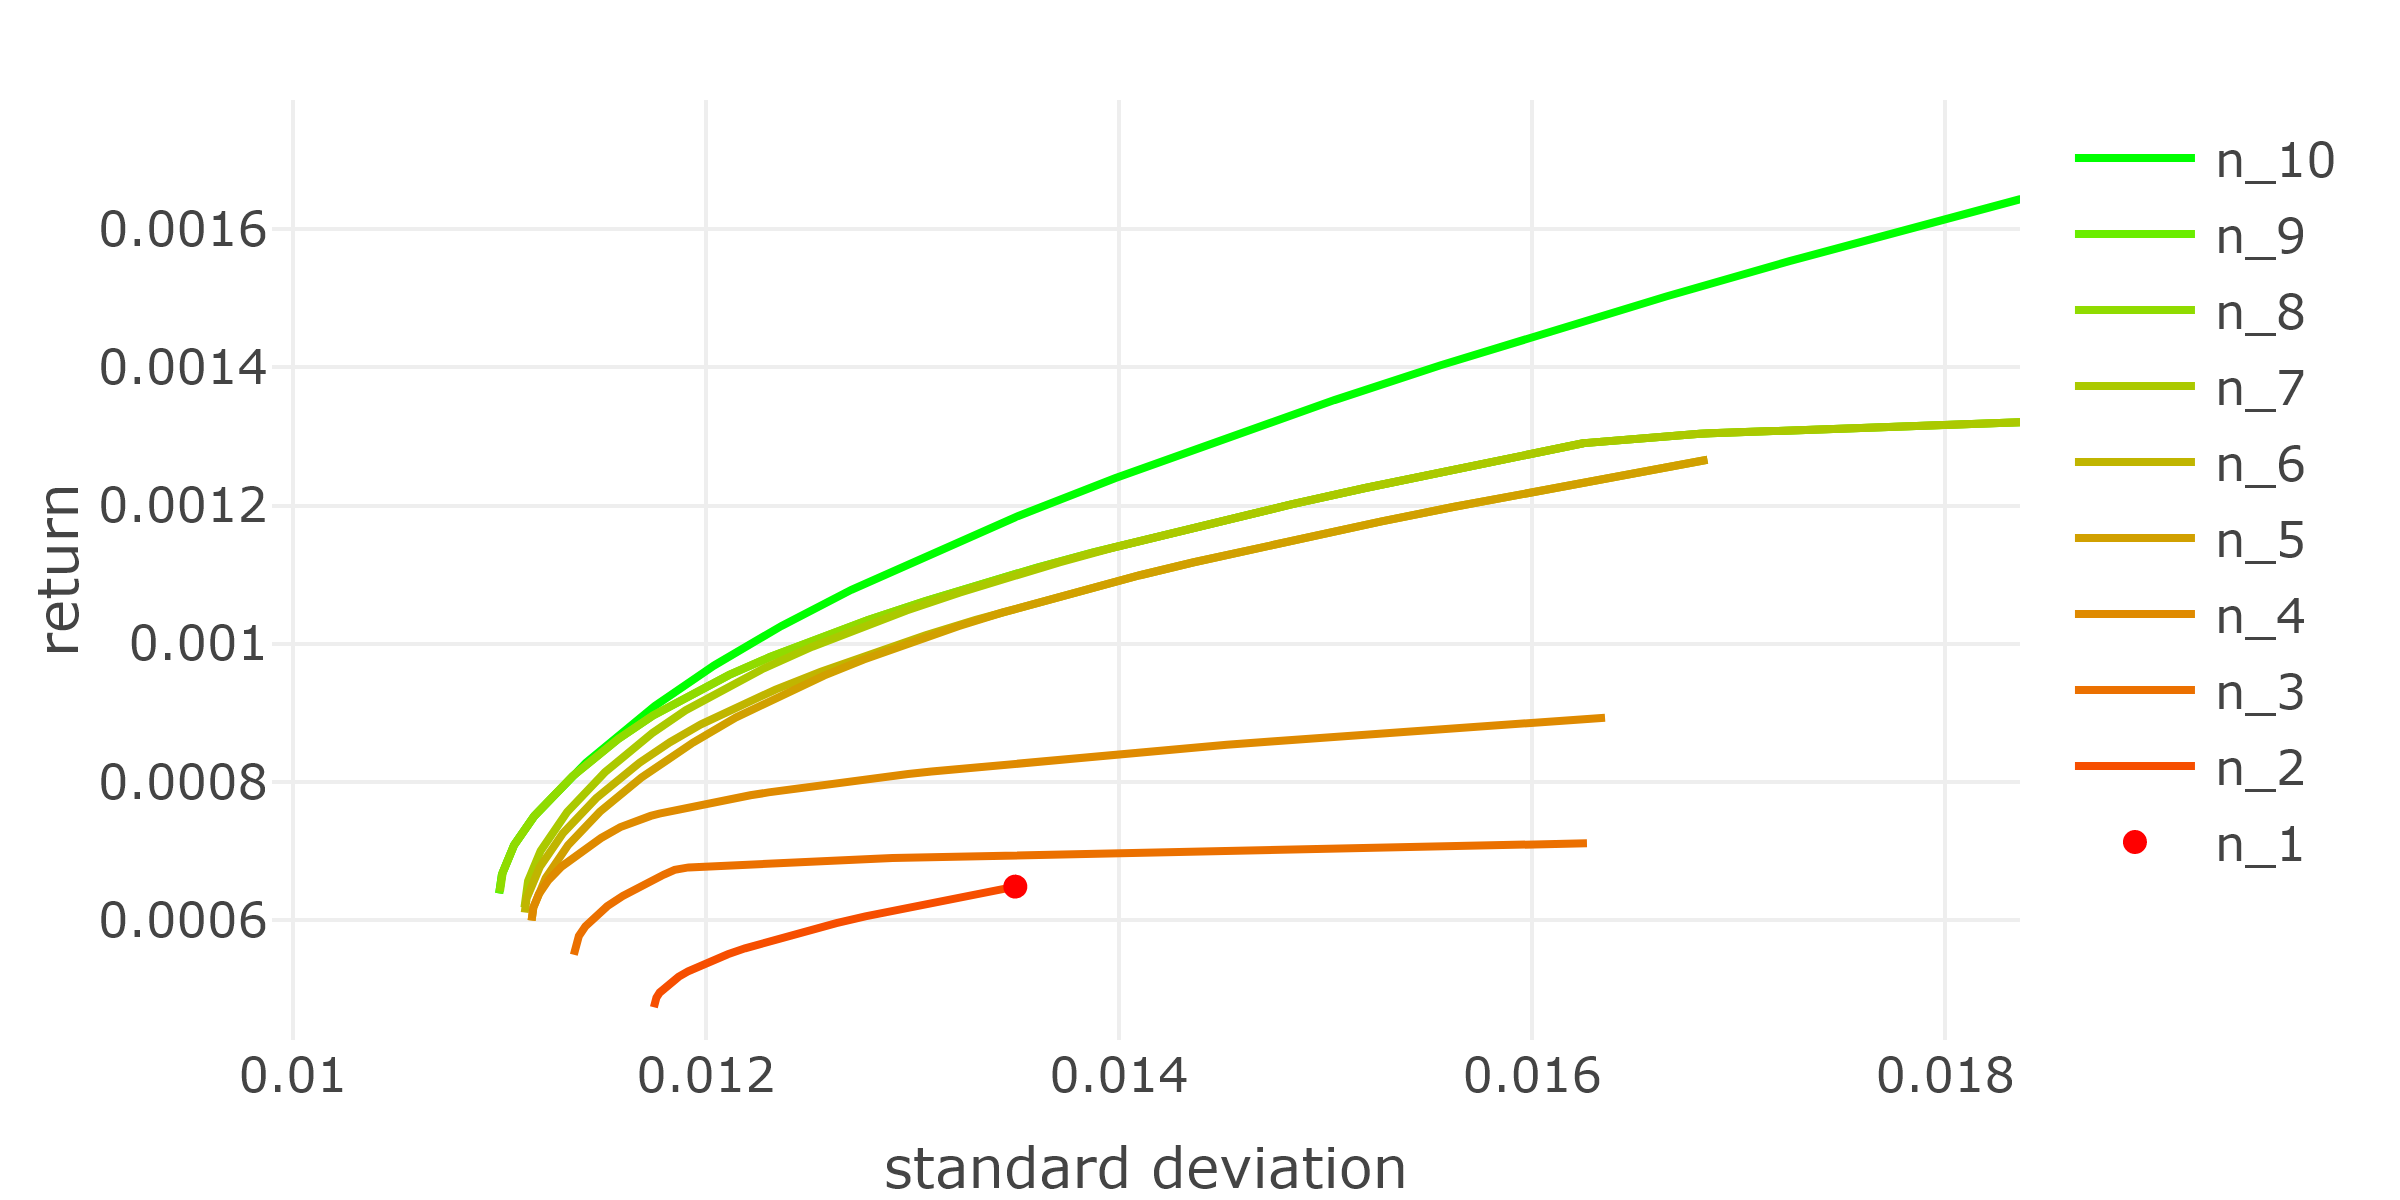
\includegraphics{Master_Thesis_files/figure-latex/unnamed-chunk-15-1} \caption{List of metaheuristics from the R package metaheuristicOpt}\label{fig:unnamed-chunk-15}
\end{figure}

These metaheuristics are used to solve the test problem defined at the beginning of this chapter. The same settings are used as for the PSO variants, i.e.~each run has a population size of 50, which corresponds to the number of particles in the swarm. The maximum iteration is 400 and each metaheuristic is run 100 times. Unlike the analysis above, only the last iteration of each run is recorded and compared. The data collected from each run of a metaheuristic are the fitness, the constraint breaks, and the run time. Aggregated for the respective metaheuristic, the 5\% and 95\% quantiles of the fitness and constraint breaks are calculated for the 100 runs, as well as the mean fitness, mean constraint breaks and mean runtime. These metrics are used to compare the respective metaheuristics in a ranking. The score calculated for this purpose is computed using the ranking in the respective category, which takes values from 1 to 24. The resulting score is a weighted sum of these individual rankings as follows:

\begin{align*}
\text{score} =& \ 3 \cdot \text{q5\_fitness\_rnk} + 2 \cdot \text{mean\_fitness\_rnk} + \text{q95\_fitness\_rnk}\\ 
&+ \text{q5\_const\_break\_rnk} + 0.5 \cdot \text{mean\_const\_break\_rnk} \\
&+ 0.5 \cdot \text{q95\_const\_break\_rnk} + 3 \cdot \text{mean\_runtime\_rnk}
\end{align*}

The score is to be interpreted in such a way that a smaller number is better than a larger one. It can be seen that the highest weight is on the 5\% quantile of fitness, as this is representative of the best solutions after repeating the metaheuristic several times. Overall, this is a subjective ranking to sort the metaheuristics and compare them with a single number. In the following chart should therefore be all the necessary information to allow the reader to form his or here own opinion:

\begin{figure}[H]
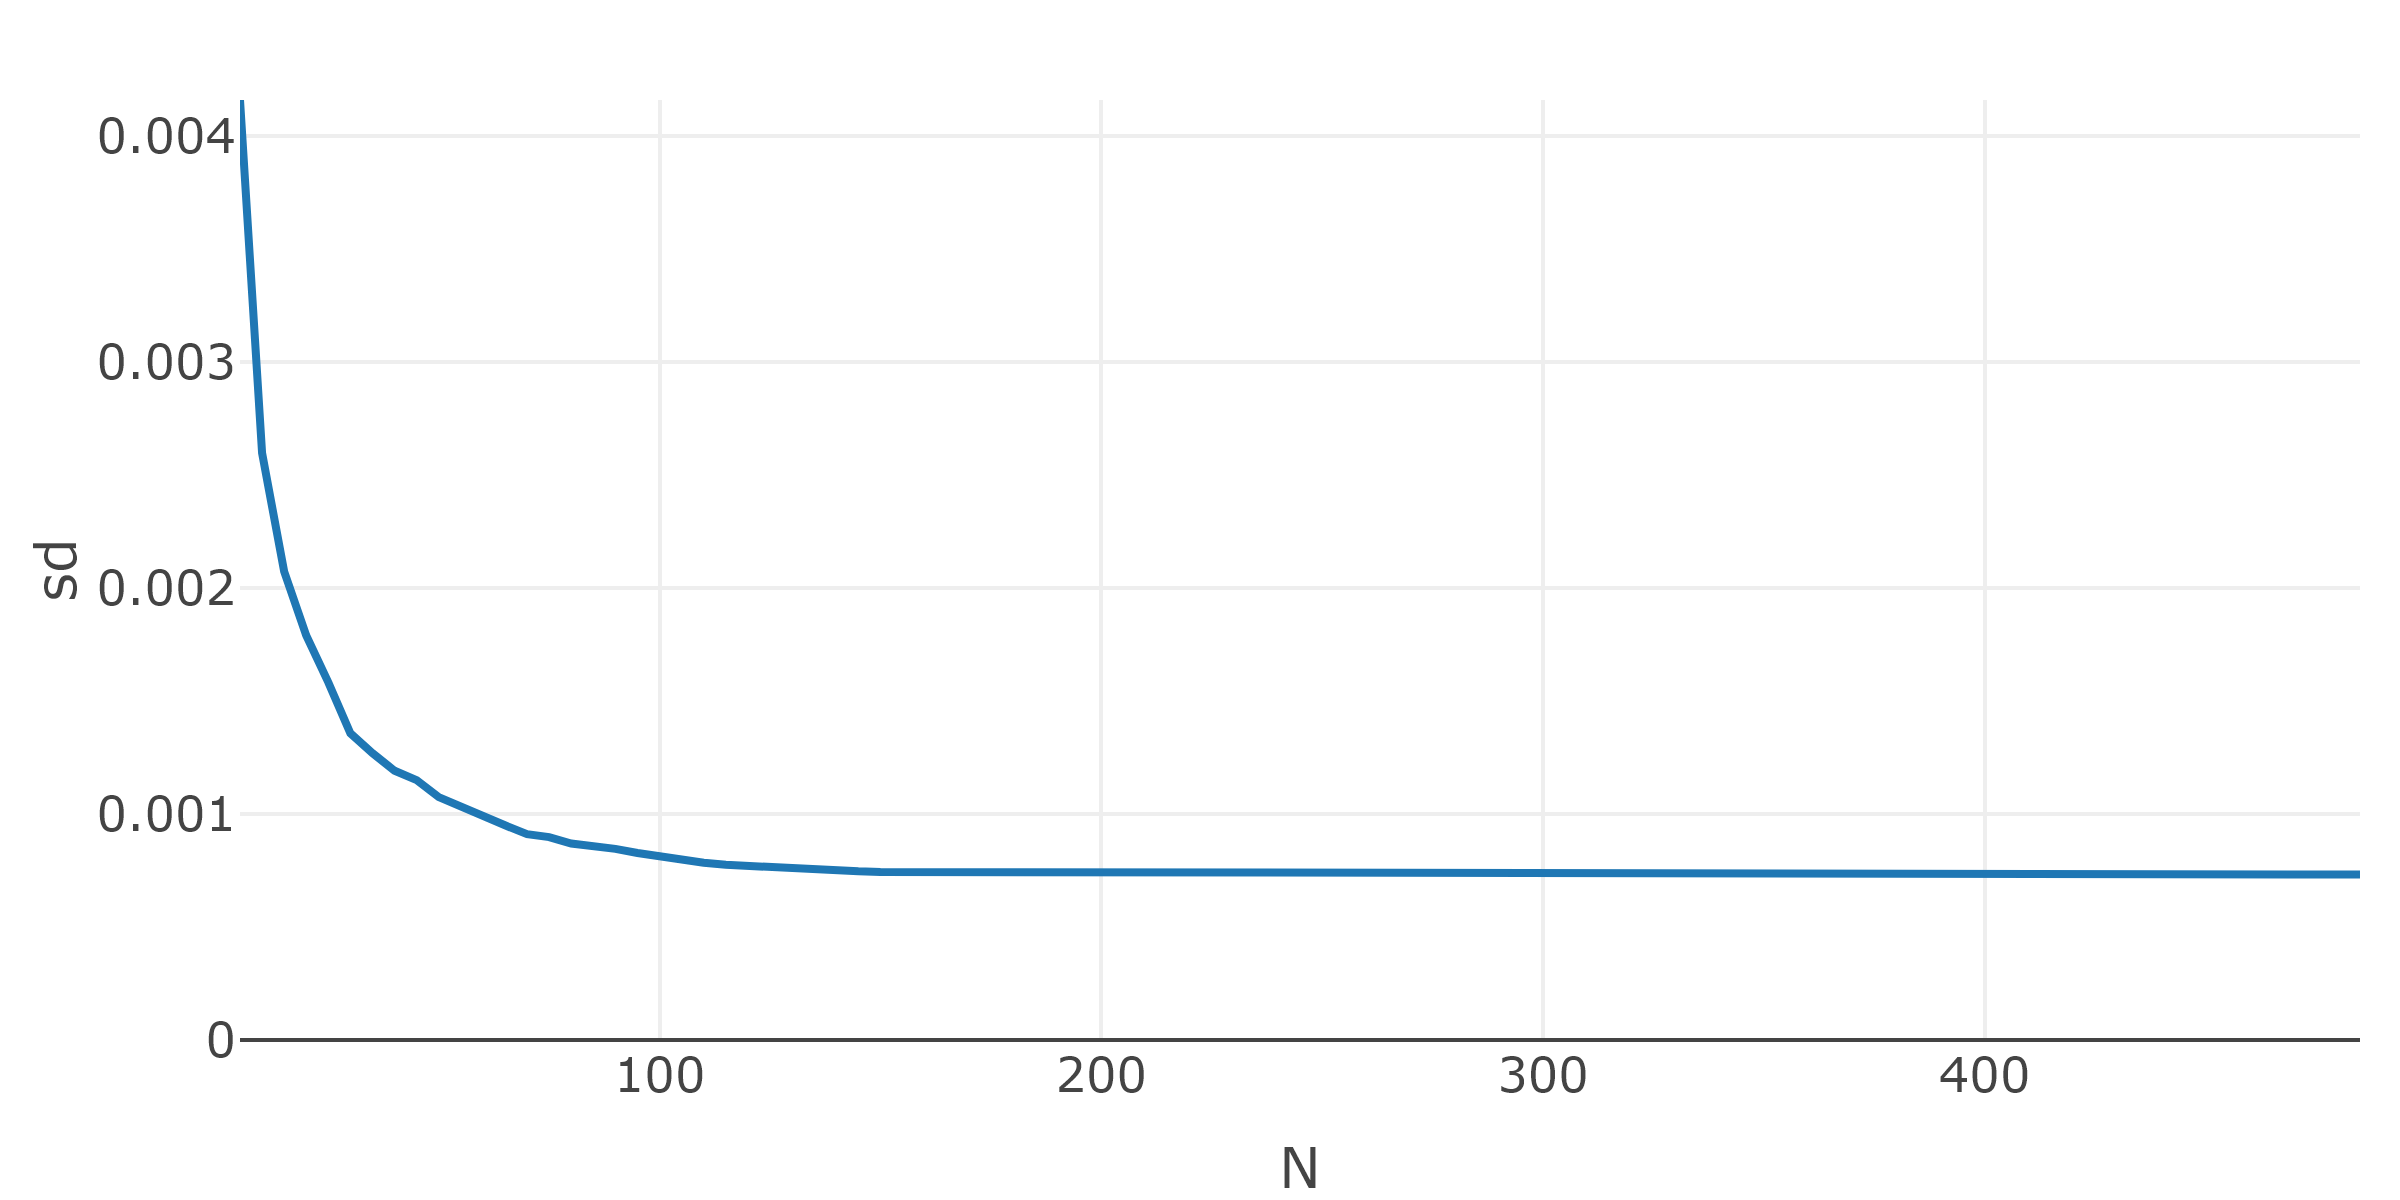
\includegraphics{Master_Thesis_files/figure-latex/unnamed-chunk-17-1} \caption{Comparison of statistics between metaheuristics}\label{fig:unnamed-chunk-17}
\end{figure}

To visualize the detailed runs, a boxplot of the important metrics fitness, constraint break and runtime was also created. In this boxplot, the individual points of each run are displayed under the respective boxes. If there are no points or boxes, it is because they have taken on too large values:

\begin{figure}[H]
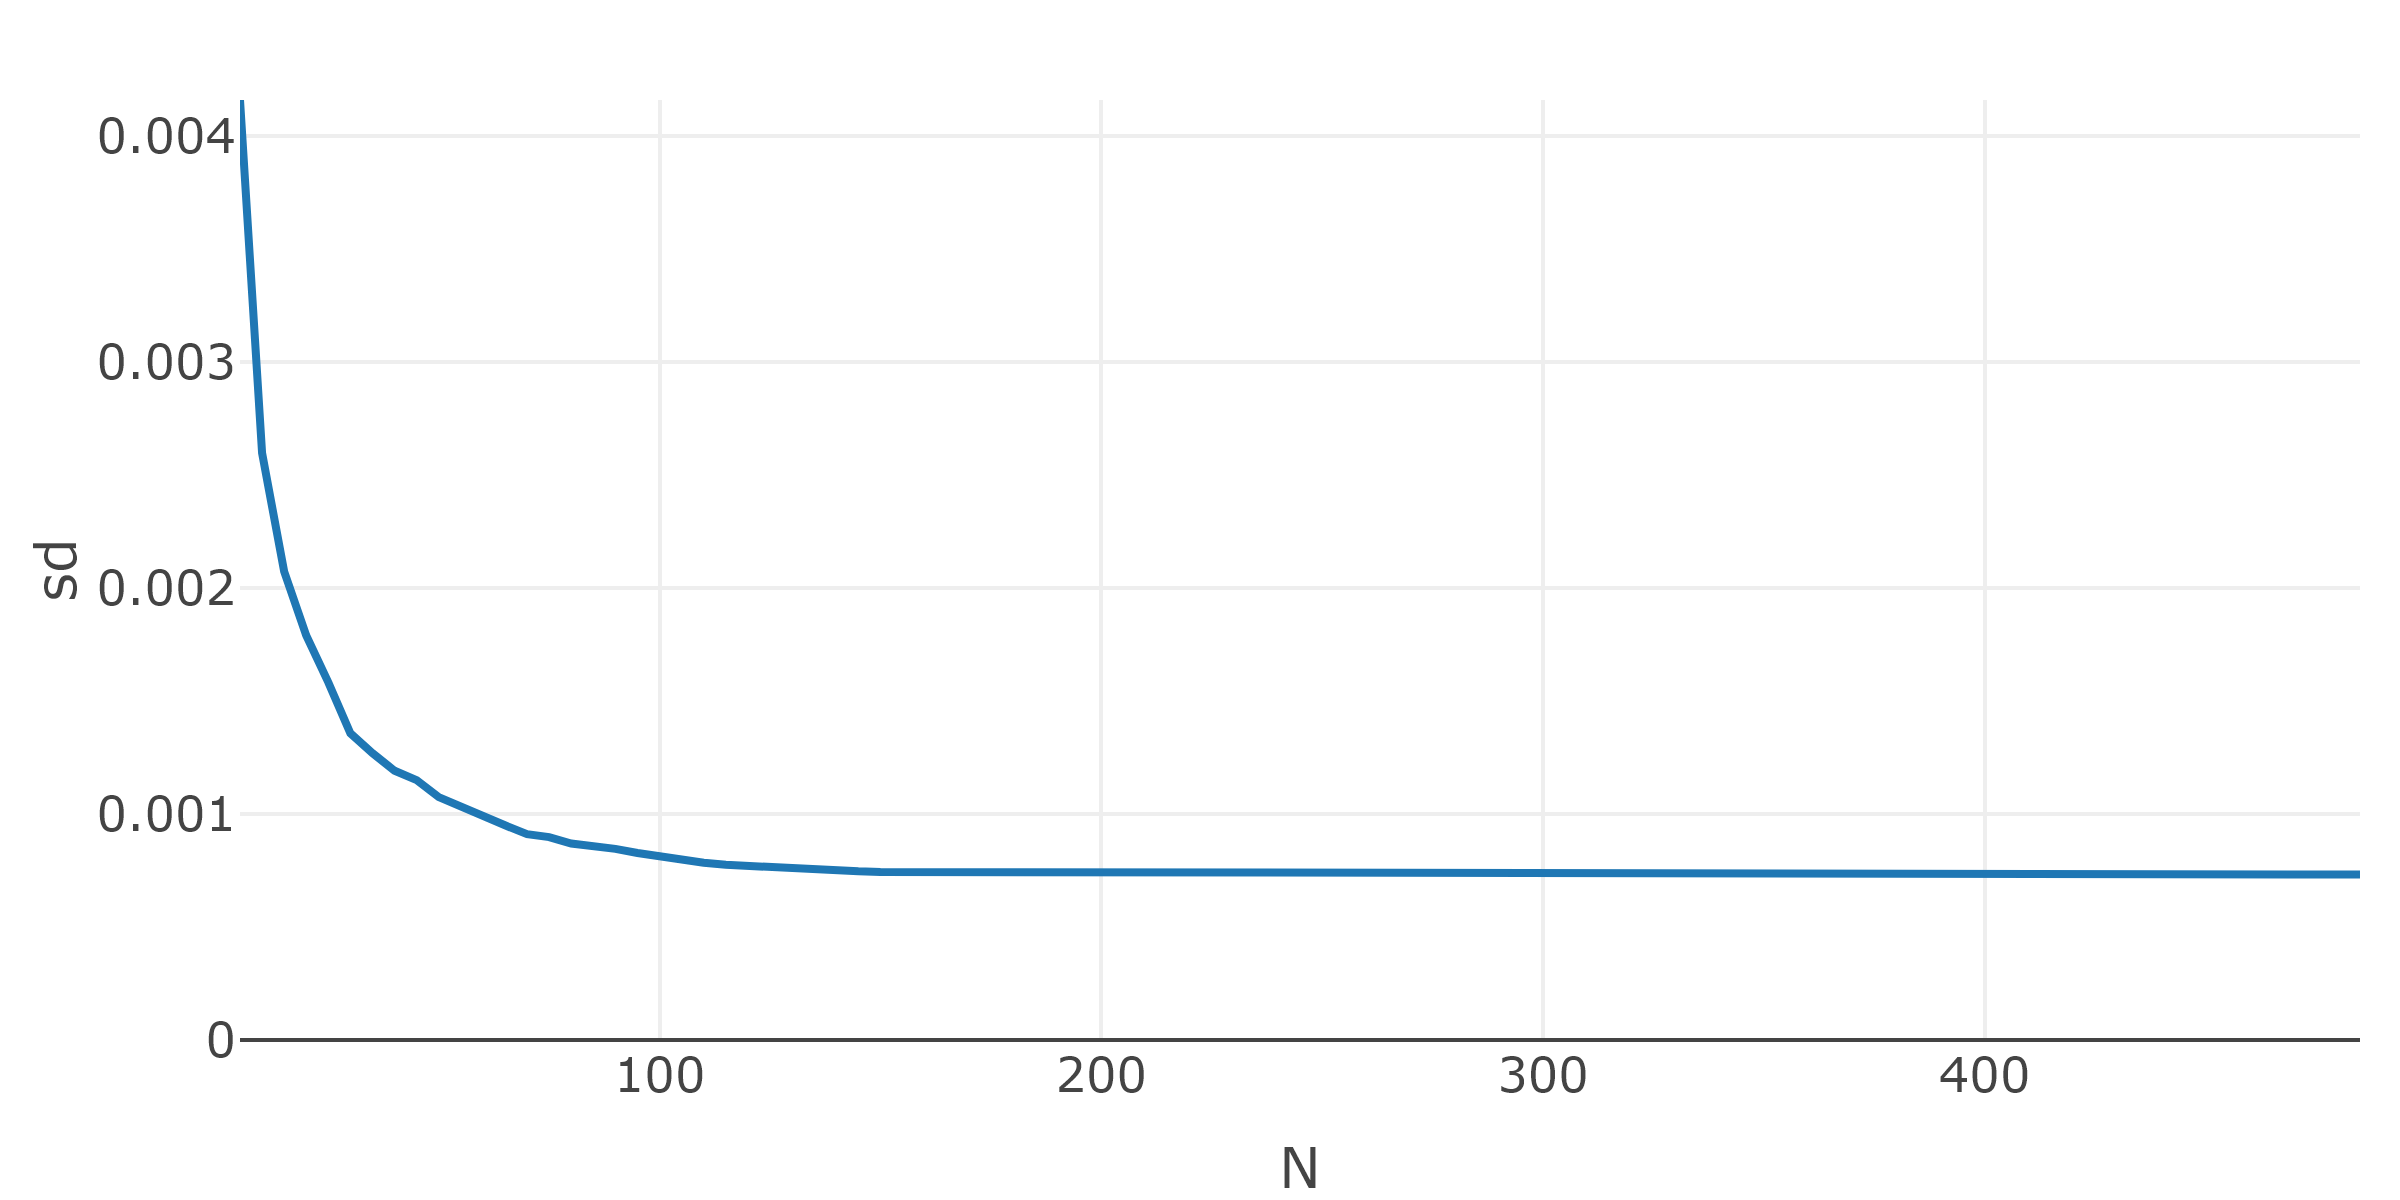
\includegraphics{Master_Thesis_files/figure-latex/unnamed-chunk-18-1} \caption{Comparison of statistics between metaheuristics with boxplots}\label{fig:unnamed-chunk-18}
\end{figure}

It can be observed that the metaheuristics from the R package \texttt{metaheuristicOpt}, consistently have a longer runtime, which is partly due to the implementation, since it does not make use of vectorial operations. Additionally it can be seen that beside the PSO and its variants also the Clonal Selection Algorithm (CLONALG) and the Ant Lion Optimizer Algorithm (ALO) reached a satisfying fitness, but had a significantly longer runtime. Overall, the self-adaptive velocity PSO (PSO-SAvel) had the best ranking, which is also confirmed by the key statistics. In addition, the PSO-SAvel has fewer hyperparameters, which is why it will be used for the backtests in the next chapter.

\hypertarget{reallife}{%
\chapter{Real Life ITP Example}\label{reallife}}

In the previous chapters, the capabilities of the PSO and the quality of its results were analyzed based on the solution of a problem at a single point in time. In practice, the stability of future outcomes at multiple points in time is of greater interest. Therefore, the next sections provide additional constraints needed to simulate real portfolios over multiple rebalancing dates, first by adding transaction costs to the problem. For the first rebalancing date, a problem is defined that simulates a portfolio manager who has a certain amount of cash and attempts to construct a portfolio from it, as described in the last section. After the first iteration, the portfolio manager must sell old assets and buy new ones. This, of course, incurs additional transaction costs and effort, so most portfolio managers consider a maximum rebalancing constraint that attempts to limit the amount of assets sold and purchased. The simulation of multiple rebalancing dates is called a backtest, which attempts to simulate the performance of a portfolio as a function of the previous portfolio and historical data for each rebalancing date. Later, a full backtest of an ITP-MSTE is evaluated and analyzed in a real-world environment.

\hypertarget{transaction-costs}{%
\section{Transaction Costs}\label{transaction-costs}}

The cost of buying or selling assets must be considered as it can have a significant impact after several years of investment. There are many different costs that can be incurred depending on the concepts of the broker, the liquidity of the assets and the type of assets. For more information, see \citep{AkGa2022} or \citep{NySe2022}. For simplicity, we focus on the situation of a retail investor using an online broker that charges a fixed fee per transaction for the U.S. stocks included in the SP500TR. Each transaction consists of one or more shares of exactly one asset, and a transaction can be either a sale or a purchase. The fixed transaction fee is set at 1 USD, as is done by the online broker Trade Republic. The PSO can account for the transaction cost by increasing the objective value, but it is difficult to make the intensity of the transaction cost value comparable to the objective value. The objective value \(v^o\) of the ITP with MSTE approach, as in section \ref{ITPMSTE}, is defined as:

\[
 v^o = \left\Vert r_{p}-r_{bm} \right\Vert_2^2 = \sum_{t=1}^T (r_{t,p}-r_{t,bm})^2.
\]

The objective value \(v^o\) is the squared tracking error or, more precisely, the squared difference of the portfolio returns \(r_p\) and the benchmark returns \(r_{bm}\). To create a comparable value \(v^{tc}\) for transaction costs, we attempt to interpret the absolute loss due to transactions as the absolute error of return \(r_{tc}\) incurred in \(t_0\) (before the first data point in \(t_1\)). This absolute error \(r_{tc}\) can be calculated by counting the required transactions divided by the net asset value \(nav\). The required transactions can be calculated by comparing the shares vector of the previous portfolio \(s^{prev}\) and the shares vector of the rebalanced portfolio \(s^{reba}\). This results in the following formula for the absolute error of return \(r_{tc}\):

\[
 r_{tc} = \frac{1 \cdot \sum_{n=1}^N g(s^{prev}_n-s^{reba}_n) }{nav}
\]

with

\[
  g(x) =    \begin{cases}
  0 &\text{, if }\ x = 0\\
  1 &\text{, else,}
  \end{cases}
\]

This results in the following transaction costs value \(v^{tc}\):

\[
v^{tc} = \left\Vert r_{tc} \right\Vert_2^2 = r_{tc}^2.
\]

The idea is to use the \(v^{tc}\) value and increase the objective value \(v^o\) of the ITP with MSTE approach, but these values are still not the same. The \(v^o\) is the sum of squared positive or negative errors and \(v^{tc}\) is a squared negative error. To increase the impact of the transaction cost, a coefficient \(k\) should increase the intensity, which leads to the following minimization problem:

\[
  min \ \  v^o + k \cdot v^{tc}.
\]

A suitable value for \(k\) could be calculated by dividing the number of training days by the number of days in the holding period increased by a factor of \(2.5\). This can be roughly interpreted as weighting the transaction cost error as the \(2.5\)-day error in the test period. For example, a 4-month training period with 96 working days and a holding period of 1 month with 24 working days yields the following value:

\[
  k = \frac{96}{24} \cdot 2.5 = 10.
\]

When the holding period is shortened, the intensity coefficient increases, which is a suitable behavior. Nevertheless, it should be analyzed and fine-tuned more.

\hypertarget{rebalancing-constraint}{%
\section{Rebalancing Constraint}\label{rebalancing-constraint}}

The rebalancing constraint restricts the changes in weights by comparing the previous portfolio weight vector \(w^{prev}\) and the rebalanced portfolio weight vector \(w^{reba}\). The value of the rebalancing should account for the weights shifted between assets and the additional weights added. Example: the previous portfolio had a weight vector \(w^{prev} = [0.5, 0.4]\) at the time before rebalancing, and the rebalanced portfolio has a weight vector \(w^{reba} = [0.8, 0.2]\). The shifted weight from the second asset to the first asset is \(0.2\) and the additional weight added is \(0.1\), resulting in a rebalancing of \(0.2+0.1=0.3\) weight. Below is the formula for calculating the rebalancing weight \(w^{rb}\) in the general case:

\[
  w^{rb} := \frac{\left\Vert w^{prev}-w^{reba} \right\Vert_1 - |\sum w^{prev} - \sum w^{reba}|}{2}+|\sum w^{prev} - \sum w^{reba}|
\]

and with a rebalancing constraint of, say, 30\%, the rebalanced portfolio is feasible if:

\[
  w^{rb} \leq 0.3.
\]

\hypertarget{objective}{%
\section{Objective}\label{objective}}

The goal is to simulate a tracking portfolio that tracks the SP500TR with a pool of 100 assets included in SP500TR over multiple rebalancing dates between 2016-05-01 and 2022-10-27 with one-month intervals. The pool of assets is created for each rebalancing date using the solve.QP approach with continuously discarding of assets as in section \ref{exampleitpsolveqp}, with a maximum of 10 assets changing on each rebalancing date to reduce forced rebalancing. All considered assets have no missing values in the training period. In addition, the solve.QP approach serves as a benchmark and the continuous solution is used as a particle position for the first rebalancing date. The tracking portfolio is solved using the self-adaptive velocity PSO from the last chapter, which yielded stable results. The tracking portfolio has the following constraints: discrete number of stocks, long only, maximum weight of 10\%, \(0.96 \leq \sum w_i \leq 0.995\), rebalancing under 30\% weight, considering transaction cost with diffrent values for \(k\), net asset value of 20000 USD, length of training period of four months and testing period of one month.

Each PSO run uses 100 particles and iterates 100 times. The PSO is repeated until the constraints are satisfied. Then it is run four more times to improve the quality of the feasible solution. Each rebalanced portfolio is simulated with the portfolio return function from section \ref{portfolioreturns} until the next rebalancing date. In each step the weights and shares of the tracking portfolio are calculated and the shares are used to calculate the weights at the next rebalancing date. If assets are missing in the next asset pool, they are sold and reduce the net asset value due to transaction costs. The same is done by buying or selling any remaining assets. A rough illustration of the process can be found in the figure on the next page.\pagebreak

\begin{figure}
\centering
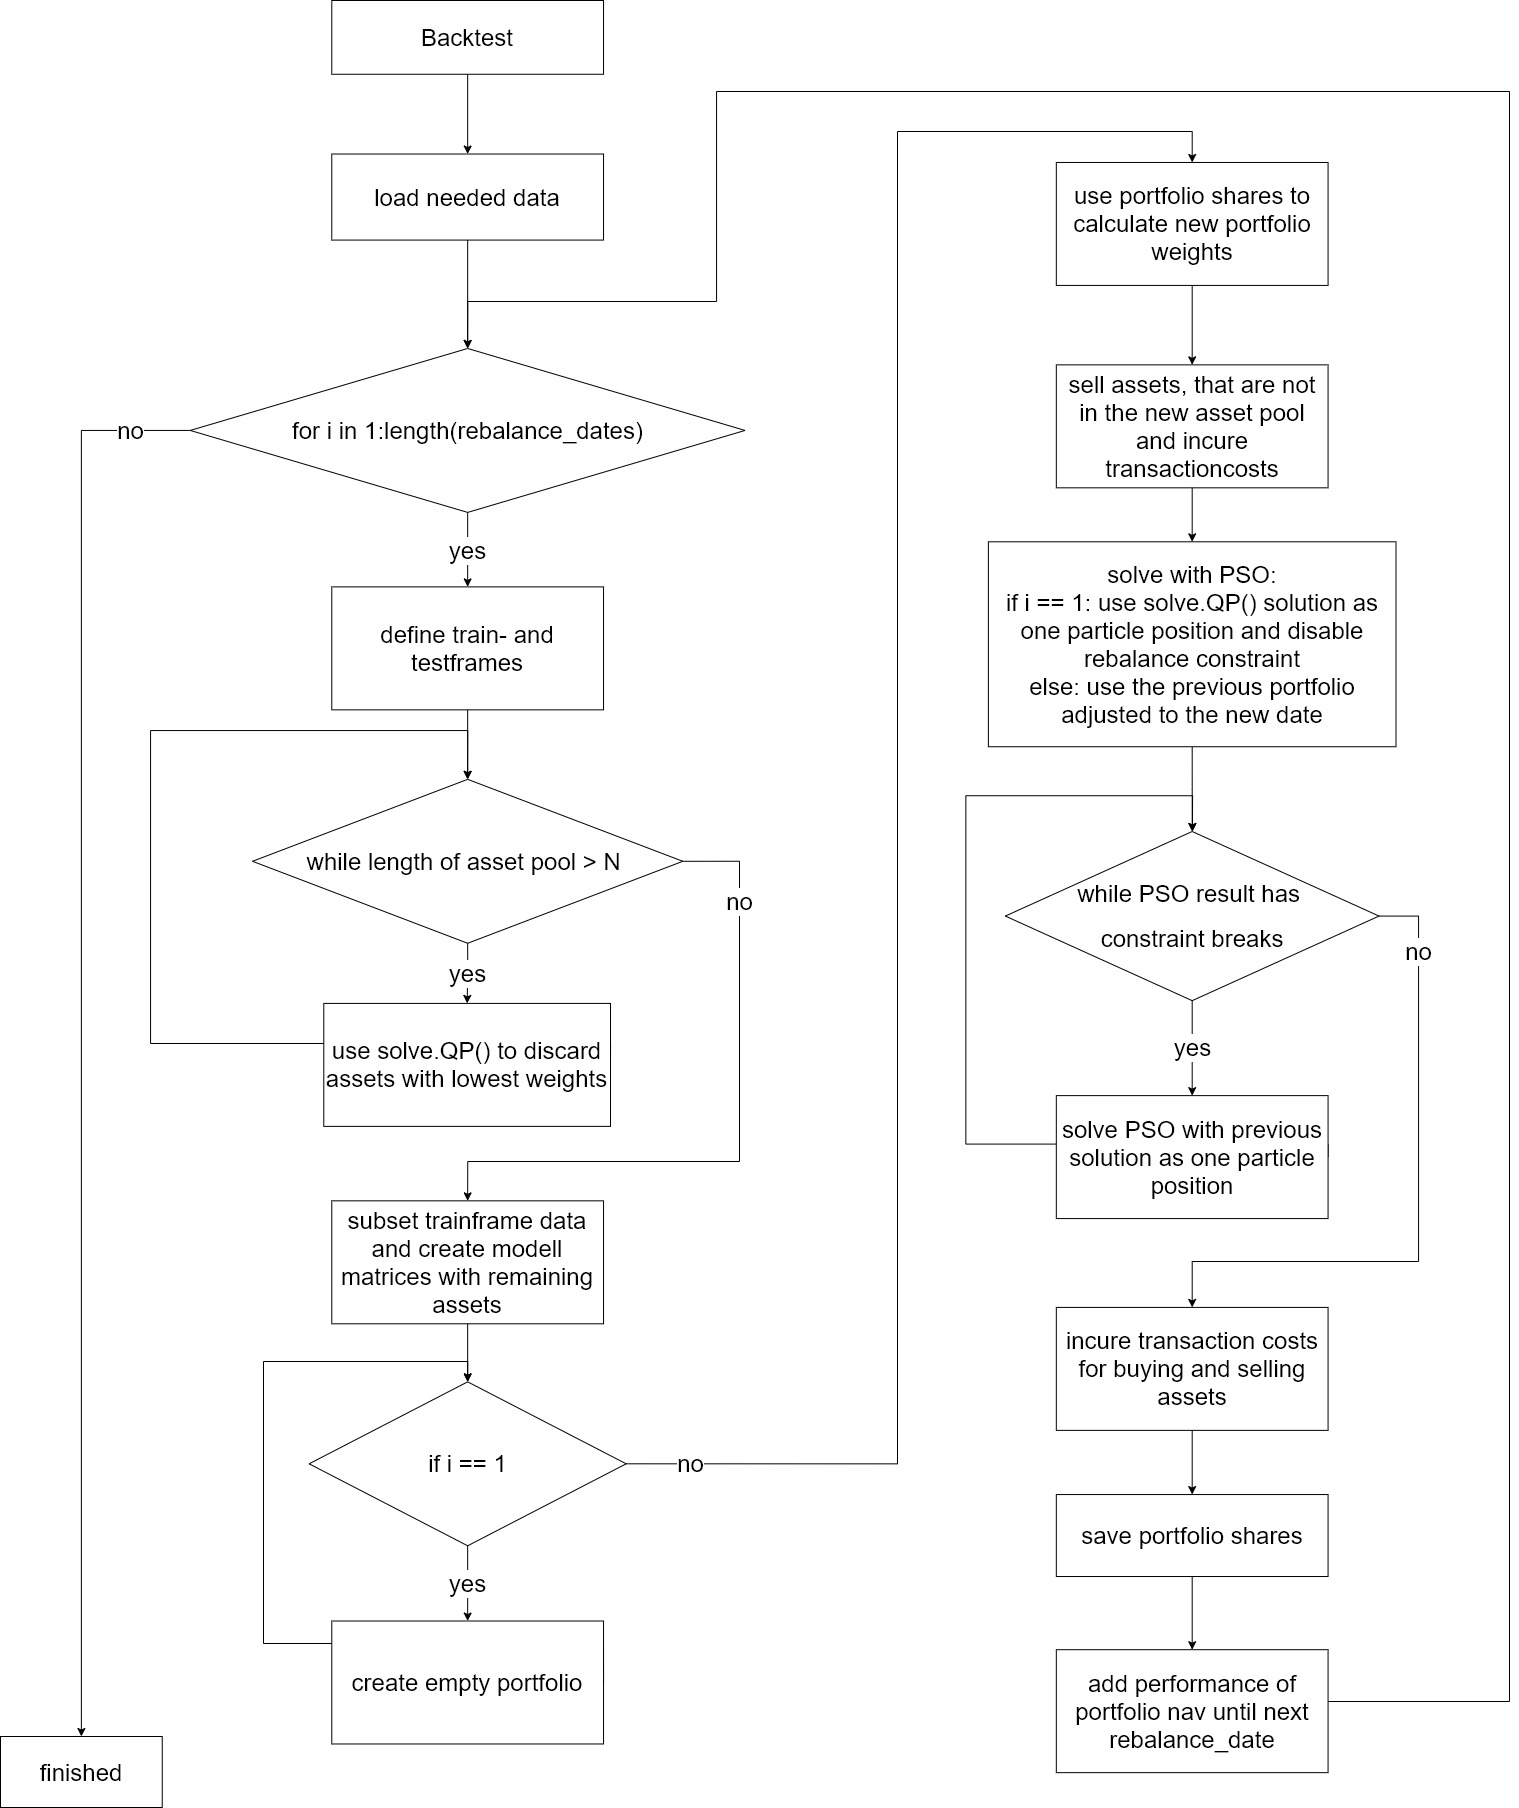
\includegraphics{img/Chapter9_PSO_Process44.jpg}
\caption{Backtest Process: visualized as a flowchart}
\end{figure}

\pagebreak

\hypertarget{complete-itp-example}{%
\section{Complete ITP Example}\label{complete-itp-example}}

The following charts visualize the test period of the whole backtests. The \texttt{QP\_MSTE\_cont} line represents the performance of the continuous solution of the ITP-MSTE objective solved with solve.QP and stays the same for all backtests. The discretized solution using the PSO is named \texttt{PSO\_MSTE\_disc} and the \texttt{PSO\_MSTE\_disc\_TR} considers all transaction costs in its performance. Everything is compared to the SP500TR which is the objective to track. Furthermore, different values for the transaction cost intensity \(k \in \{0, 10, 20, 30\}\) of the individual backtests are used, indicated in the legends as \texttt{0tc}, \texttt{10tc}, \texttt{20tc} and \texttt{30tc}.

Backtest for \(k=0\):

\begin{figure}[H]
\includegraphics{Master_Thesis_files/figure-latex/93-1} \caption{Comparison of the cumulative daily returns of the backtests with the transaction cost value k=0}\label{fig:93}
\end{figure}

and the statistics of the discretized PSO with considered transaction costs are:

\begin{figure}[H]
\includegraphics{Master_Thesis_files/figure-latex/94-1} \caption{Comparison of the statistics of the backtests with the transaction cost value k=0}\label{fig:94}
\end{figure}

Backtest for \(k=10\):

\begin{figure}[H]
\includegraphics{Master_Thesis_files/figure-latex/95-1} \caption{Comparison of the cumulative daily returns of the backtests with the transaction cost value k=10}\label{fig:95}
\end{figure}

and the statistics of the discretized PSO with considered transaction costs are:

\begin{figure}[H]
\includegraphics{Master_Thesis_files/figure-latex/96-1} \caption{Comparison of the statistics of the backtests with the transaction cost value k=10}\label{fig:96}
\end{figure}

Backtest for \(k=20\):

\begin{figure}[H]
\includegraphics{Master_Thesis_files/figure-latex/97-1} \caption{Comparison of the cumulative daily returns of the backtests with the transaction cost value k=20}\label{fig:97}
\end{figure}

and the statistics of the discretized PSO with considered transaction costs are:

\begin{figure}[H]
\includegraphics{Master_Thesis_files/figure-latex/98-1} \caption{Comparison of the statistics of the backtests with the transaction cost value k=20}\label{fig:98}
\end{figure}

Backtest for \(k=30\):

\begin{figure}[H]
\includegraphics{Master_Thesis_files/figure-latex/99-1} \caption{Comparison of the cumulative daily returns of the backtests with the transaction cost value k=30}\label{fig:99}
\end{figure}

and the statistics of the discretized PSO with considered transaction costs are:

\begin{figure}[H]
\includegraphics{Master_Thesis_files/figure-latex/910-1} \caption{Comparison of the statistics of the backtests with the transaction cost value k=30}\label{fig:910}
\end{figure}

Since each backtest depends on different previous portfolios, further backtests are needed to draw reliable inferences about the observed phenomena. That being said, it can be observed in this particular case that an increase in \(k\) tends to lower the average transaction costs. This can be seen in the comparison of the statistics of the individual backtests, since there, except for \(k=30\), a higher \(k\) leads to lower average transaction costs. To analyze this in more detail, the loss due to transaction costs of each backtest is visualized in the following chart:

\begin{figure}[H]
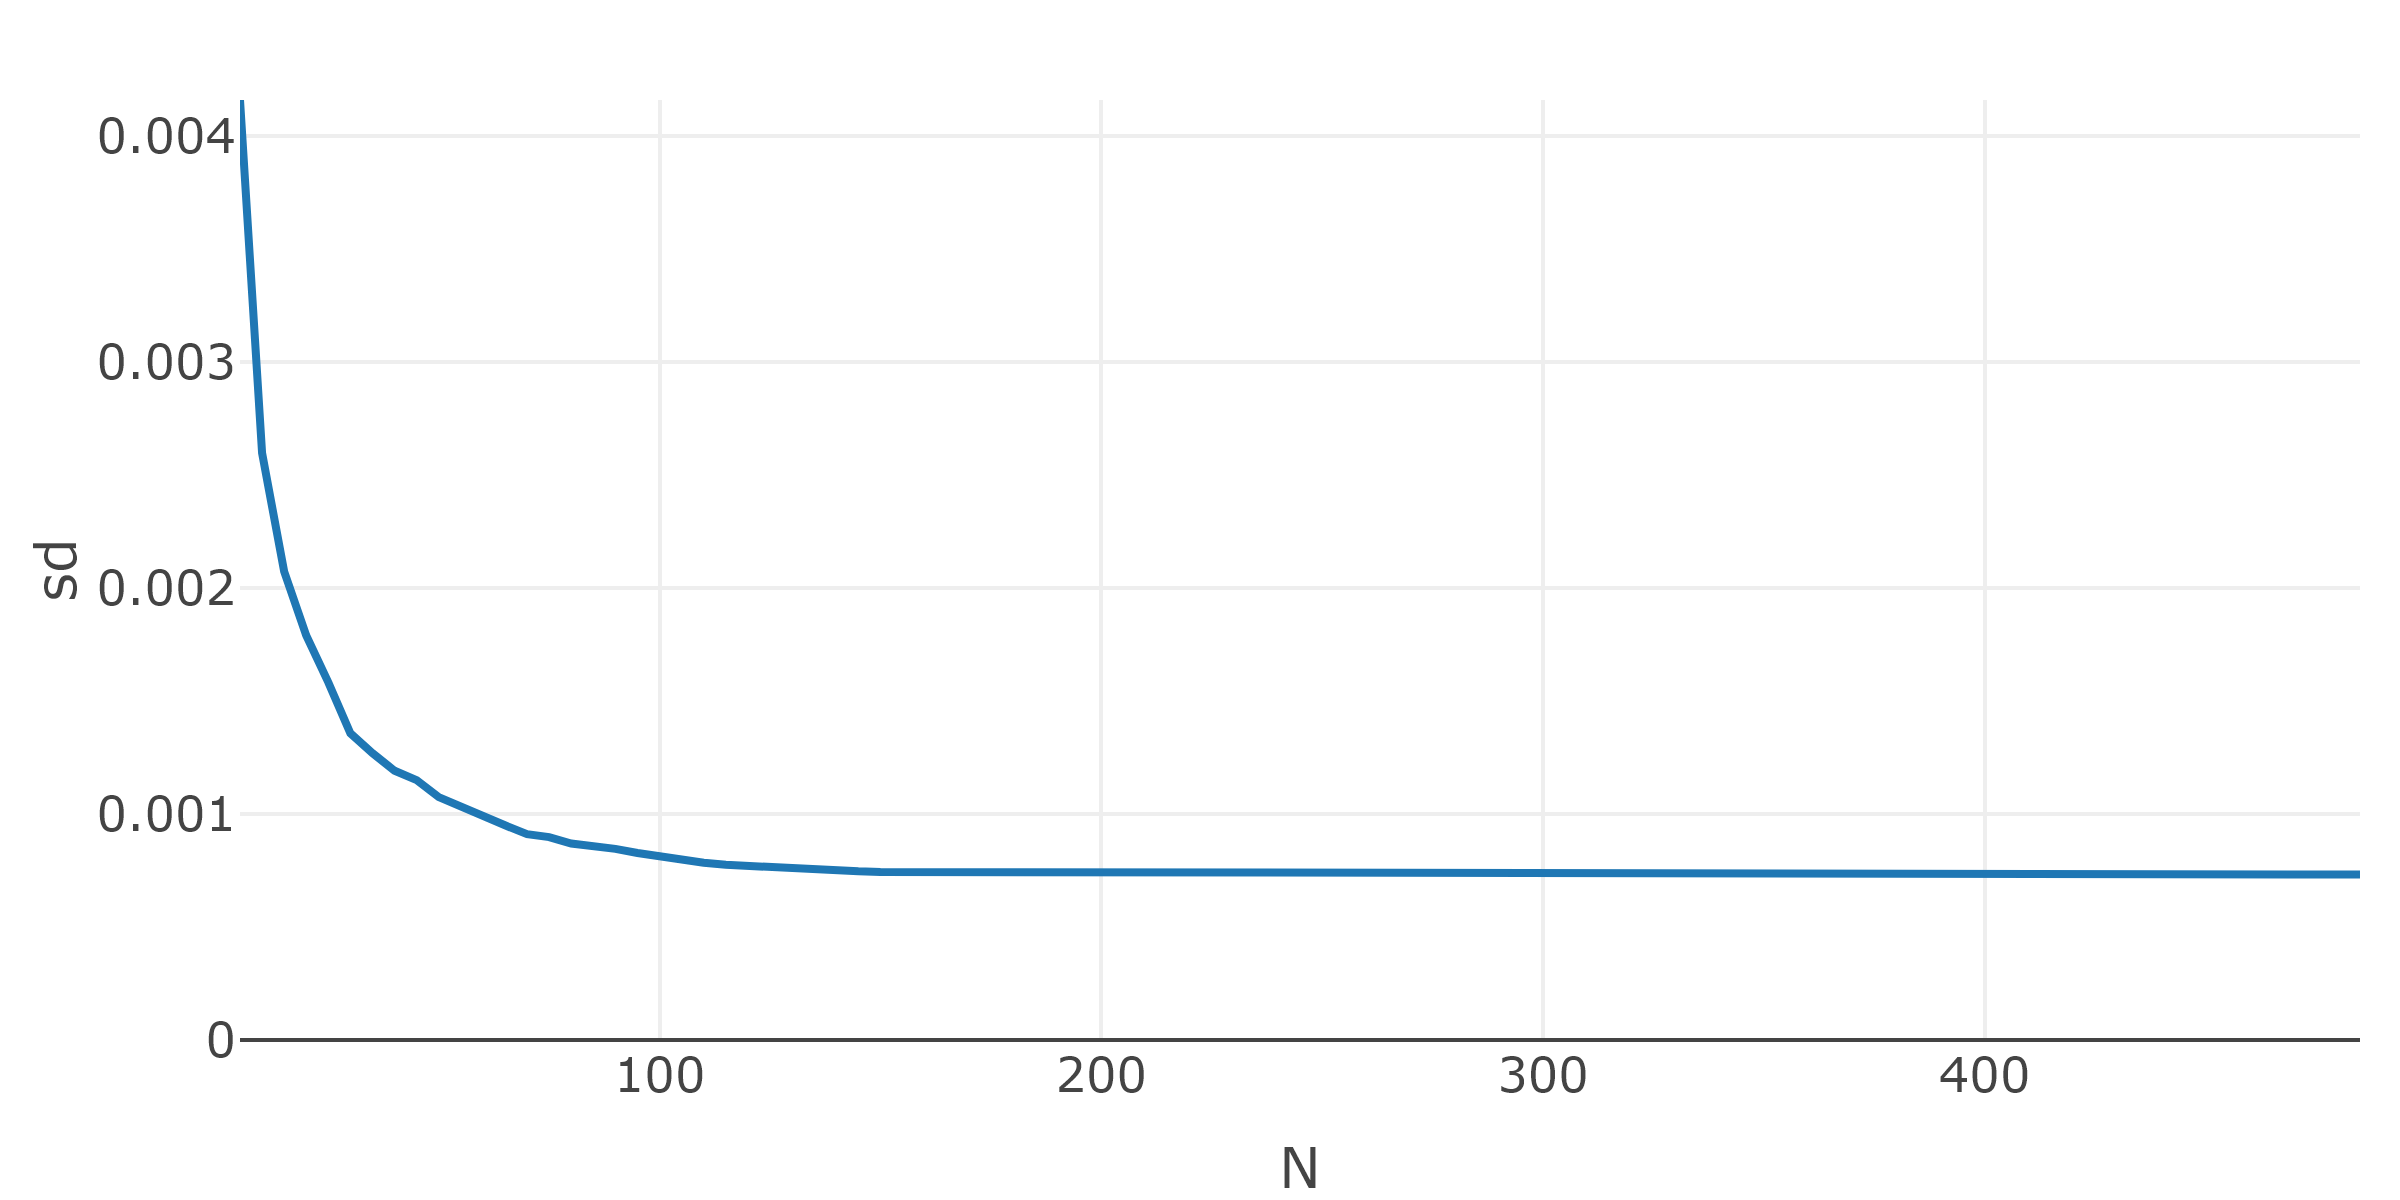
\includegraphics{Master_Thesis_files/figure-latex/unnamed-chunk-19-1} \caption{Cumulative daily return loss of the discrete PSO backtests due to transaction costs with respect to the different values of k}\label{fig:unnamed-chunk-19}
\end{figure}

Another interesting result is that the continuous \texttt{solve.QP} approach with a pool of 100 assets had a slightly higher performance than the SP500TR, suggesting that the asset pool in that particular period consists of assets that performed relatively well. This can be inspected in the following performance chart, comparing only the \texttt{solve.QP} approach and the SP500TR:

\begin{figure}[H]
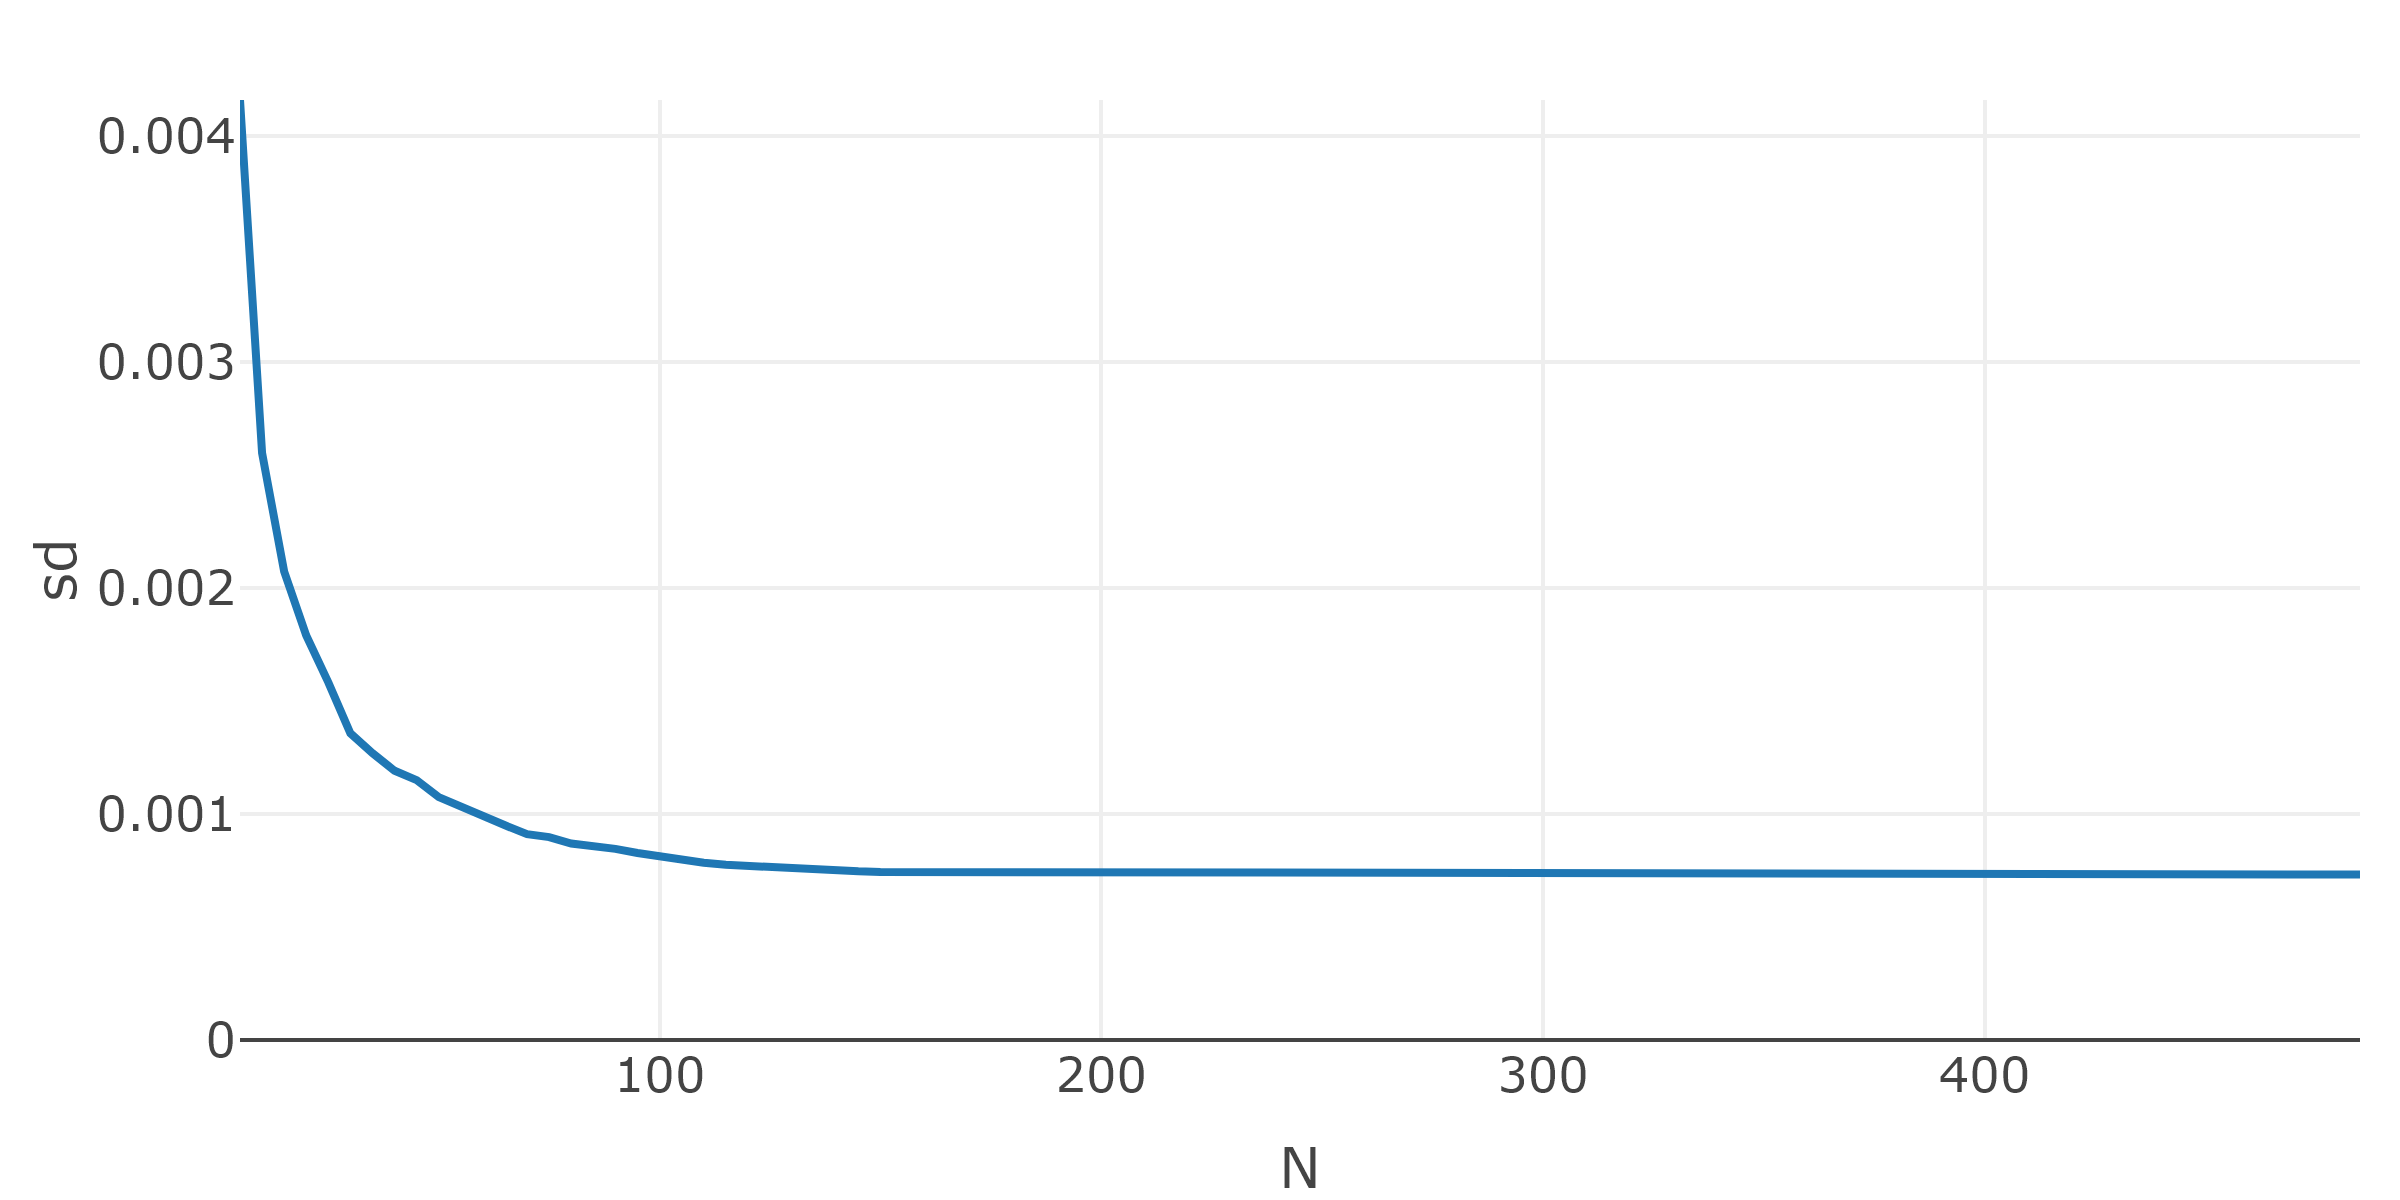
\includegraphics{Master_Thesis_files/figure-latex/unnamed-chunk-20-1} \caption{Comparison of cumulative daily returns of the continuous backtest performed with solve.QP and the SP500TR}\label{fig:unnamed-chunk-20}
\end{figure}

\hypertarget{future-research}{%
\chapter{Future Research}\label{future-research}}

The variants of the Particle Swarm Optimization were examined for their efficacy in solving the index tracking problem. The local PSO and the self-adaptive velocity PSO were found to be particularly effective, as they increase the diversity within the swarm and prevent premature convergence in local minima. Additionally, the self-adaptive velocity PSO offers the advantage of reducing the number of hyperparameters, making it capable of solving a wide range of problems without the need for extensive fine-tuning. The implementation of the self-adaptive velocity PSO, as described in \citep{FaYa2014}, was found to be effective, but further research is needed to determine whether it can be improved by combining it with the local variant.

A backtesting study was conducted in the final chapter, evaluating the practical application of the index tracking problem for retail investors. The results were promising, but further evaluation is necessary to confirm the stability of the results, given the path-dependent nature of the portfolios.

\hypertarget{conclusion}{%
\chapter{Conclusion}\label{conclusion}}

This thesis has been concerned with the analysis and testing of the PSO. The focus has been on optimization problems in the field of quantitative portfolio management. In practice, it is relevant to solve these kind of optimization problems with the same complexity as in real life, which is made possible by the PSO. It has been shown that even complex optimization problems can be solved in a stable manner.

It was shown in chapter \ref{activevspassive} that more and more investors invest in passive managed funds, as they are more stable over time and have lower costs. To ensure competitiveness, it is important that quantitative strategies are automated as much as possible. The use of PSO in solving optimization problems in quantitative portfolio management is particularly relevant in this context, as it allows for the efficient and effective solution of these complex problems.

In chapter \ref{challenges}, various optimization problems commonly encountered in the realm of quantitative investment strategies within passive investment were examined and presented through the use of examples. One of the issues analyzed was the mean-variance portfolio (MVP) problem, the solution of which yields an optimal portfolio in terms of risk and return. Additionally, the topic of index tracking problem (ITP) was introduced, which aims to create a tracking portfolio that closely follows its benchmark. It was demonstrated that it is beneficial to achieve the ITP by minimizing the mean square tracking error, which was succinctly referred to as ITP-MSTE.

In chapter \ref{analyticalsolver}, a quadratic optimizer called solve.QP was used to solve the quadratic problems with their constraints in the continuous case of the MVP problem and the ITP-MSTE. The solve.QP was also used as a benchmark to test the quality of the PSO in the following chapter \ref{spso}. It was found that although the PSO requires significantly more computation time, the results are often close to the solve.QP solution. In addition, the standard PSO was explained in detail and illustrated using visualizations and WebApps. It was shown how the penalty method works to take constraints into account during optimization. Furthermore, the convergence behavior of the standard PSO was analyzed, leading to the conclusion that the standard PSO is not a local search algorithm, but can be transformed into a local and also a global search algorithm by applying small modifications. It has been shown that PSO leads to stable results in the chosen financial optimization problems, provided that sufficient computing time is used.

Since in reality a portfolio consists of integer numbers of assets, it was shown that quadratic optimizers and subsequent rounding are not sufficient for discrete problems. For the PSO, it was shown how to deal with such discrete problems and then the discrete ITP-MSTE was solved, yielding stable results. This is particularly important in the context of quantitative portfolio management, as many real-world problems involve discrete variables.

In the next chapter \ref{psovariants} different variants of the PSO were analyzed and compared with the standard PSO. It was found that the local PSO and the self-adaptive velocity PSO are the best variants to solve the discrete ITP-MSTE. In addition, the created PSO variants were compared with other metaheuristics applied to the same problem. It was found that the local PSO and the self-adaptive velocity PSO are better than the other metaheuristics. Since the self-adaptive velocity PSO has no hyperparameters that need to be adjusted, it was tested extensively in the following chapter.

In the final chapter of this thesis, the self-adaptive velocity PSO algorithm was applied in a practical scenario. A simulation was conducted in which the optimization problem of a private investor who regularly rebalances their portfolio on a monthly basis was considered. To accurately simulate the conditions of a private investor who adjusts their portfolio on a monthly basis, the ITP-MSTE model was designed to consider the transaction costs and the maximum limit of rebalancing allowed in a single month. The self-adaptive velocity PSO was then utilized to solve this optimization problem and was repeatedly executed until no constraints were violated, which was achieved in all cases. The results of this simulation indicate that the model has been solved effectively. However, further extensive testing is required to accurately assess the stability of the proposed model, as the portfolios in the backtests are path dependent.

Overall, it has been demonstrated that PSO can effectively yield stable results in financial optimization problems when given sufficient computational resources. The simplicity of formulating even complex problems is a key advantage of this method. As the financial industry continues to evolve and place increasing emphasis on automation of quantitative strategies, it is likely that optimization techniques like PSO will become increasingly prevalent.

  \bibliography{book.bib,packages.bib}

\includepdf[pages=-]{Master_Thesis_Erklärung.pdf}

\end{document}
